\documentclass{article}

\usepackage{fancyhdr}
\usepackage{amsmath}
\usepackage{amsthm}
\usepackage{amssymb}
\usepackage{amsfonts}
\usepackage{tikz}
\usepackage{MnSymbol}

\newcommand{\w}[0]{\omega}
\newcommand{\z}[0]{\zeta}
\newcommand{\Q}[0]{\mathbb{Q}}
\newcommand{\R}[0]{\mathbb{R}}
\newcommand{\F}[0]{\mathbb{F}}
\newcommand{\C}[0]{\mathbb{C}}
\newcommand{\A}[0]{\mathbb{A}}
\newcommand{\Z}[0]{\mathbb{Z}}
\newcommand{\Zmult}[1]{\mathbb{Z}_{#1}^{*}}
\newcommand{\p}[0]{\mathfrak{p}}
\newcommand{\q}[0]{\mathfrak{q}}
\newcommand{\zquad}[1]{\mathbb{Z}[\sqrt{#1}]}
\newcommand{\qext}[1]{\mathbb{Q}[#1]}
\newcommand{\zext}[1]{\mathbb{Z}[#1]}
\newcommand{\trace}[1]{\text{Tr}(#1)}
\newcommand{\image}[1]{\text{Im}(#1)}
\newcommand{\norm}[0]{\text{N}}
\newcommand{\diff}[1]{\text{diff}\ #1}
\newcommand{\disc}[1]{\text{disc}(#1)}
\newcommand{\kernel}[0]{\text{kern}}
\newcommand{\modequiv}[3]{#1 \equiv #2\ (#3)}
\newcommand{\modnotequiv}[3]{#1 \not\equiv #2\ (#3)}
\newcommand{\gal}[2]{\text{Gal}(#1 / #2)}
\newcommand{\ringofintegers}[1]{\mathbb{A} \cap #1}
\newcommand{\legendre}[2]{\genfrac{(}{)}{}{}{#1}{#2}}

\newtheorem{theorem}{Theorem}[section]
\newtheorem{lemma}{Lemma}

\begin{document}

\section*{Chapter 1}

\begin{enumerate}
\item [23.]  If $\modequiv{\beta}{\gamma}{p}$, then $\beta - \gamma = \delta p$; therefore $\overline{\beta - \gamma} = \bar{\delta}\bar{p}$, so $\bar{\beta} - \bar{\gamma} = \bar{\delta}p$; therefore $\modequiv{\bar{\beta}}{\bar{\gamma}}{p}$.

\item [24.]  $(\beta + \gamma)^p = \beta^p + \gamma^{p} + \sum_{i=1}^{p - 1} \binom{p}{i} \beta^{i} \gamma^{p - i}$; each of the terms in the summation  are divisible by $p$ and so are 0 mod $p$, so $\modequiv{(\beta + \gamma)^{p}}{\beta^{p} + \gamma^{p}}{p}$.

\item [25.]  Take $\alpha \in \Z[\w]$; then $\alpha = a_{p-2}\w^{p-2} + \ldots + a_0$.  By Exercise 1.24 \[ \modequiv{\alpha^{p}}{a_{p-2}^{p}\w^{p(p-2)} + \ldots + a_0^{p}}{p} \] As $\w^{p} = 1$, \[ \modequiv{\alpha^{p}}{a_{p-2}^{p} + \cdots + a_0^{p} \in \Z}{p} \]

\item [26.] Suppose $\modequiv{x + y\w}{u\alpha^{p}}{p}$; by Exercise 1.25, $\modequiv{x + y\w}{um}{p}$ for some $m \in Z$.  Applying Exercise 1.23 we have $\modequiv{x + y\w^{-1}}{\bar{u}m}{p}$; therefore $\modequiv{x + y\w}{(u/\bar{u})(x + y\w^{-1})}{p}$.  By the lemma on units $u / \bar{u} = \w^{k}$ for some $k$, so $\modequiv{x + y\w}{(x + y\w^{-1})\w^{k}}{p}$ for some $0 \le k < p$.

\item [27.] Multiplying $(x + y\w^{-1})\w^{k}$ through by $\w^k$ and subtracting gives an expression that $\equiv$ 0 mod $p$; $\modequiv{x + y\w - y\w^{k-1} - x\w^{k}}{0}{p}$.  By Exercise 22 $p$ must divide all coefficients of this expression.  However $x, y \not\mid p$.  If $k = 0$ or $k > 1$ then the constant term of the expression would be $x$, a contradiction.

\item [28.] Taking $k$ the above expression reduces to $\modequiv{x + y\w - y - x\w = (x - y) + (y - x)\w}{0}{p}$; by Exercise 22, $p \mid x - y$ and $p \mid y - x$; therefore $\modequiv{x}{y}{p}$.

\item [29.]  We use Sage to avoid multiplying the terms out by hand:
\begin{verbatim}
sage: K.<w> = CyclotomicField(23)
sage: e1 = (1+w^2+w^4 + w^5 + w^6 + w^10 + w^11)
sage: e2 = (1 + w + w^5 + w^6 + w^7 + w^9 + w^11)
sage: e1 * e2
2*w^17 + 2*w^16 + 2*w^15 + 2*w^13 + 2*w^12
+ 6*w^11 + 2*w^10 + 2*w^9 + 2*w^7 + 2*w^6 + 2*w^5
\end{verbatim}

\end{enumerate}

\section*{Chapter 2}

\begin{enumerate}

\item[1. (a)] Show every number field of degree 2 over $\mathbb{Q}$ is one of the quadratic fields.

Let $K$ be a number field of degree 2, and $f(x) = x^2 + px + q$ be its minimum polynomial over $\mathbb{Q}$.  Since $p, q \in \mathbb{Q}$ we can multiply through to clear the denominators and give us a polynomial $g(x) = ax^2 + bx + c$ over $\mathbb{Z}$ with the same roots as $f(x)$.  Therefore $K = \mathbb{Q}[\sqrt{b^2 - 4ac}]$ is a quadratic field for $m = b^2 - 4ac$.

\item[1. (b)] Suppose $K = \mathbb{Q}[\sqrt{m}]$ contains $\sqrt{n}$ for $n$ a squarefree integer.  Since $K$ has the basis $\{1, \sqrt{m}\}$, so $\sqrt{n} = p + q\sqrt{m}$ for $p, q \in \mathbb{Q}$. Therefore $n = p^2 + 2pq\sqrt{m} + q^2m$, so either $p = 0$ or $q = 0$.

If $p = 0$, then $\sqrt{n} = q\sqrt{m}$ and so $\sqrt{n} / \sqrt{m} = q$.  This can only happen if $q = 1$, meaning $m = n$.

If $q = 0$, then $\sqrt{n} = p$, which can only happen if $p$ is also an integer, contradicting $n$ squarefree.

Therefore the quadratic fields are each distinct.

\item[2.]
    Let $I$ be the ideal generated by $2$ and $1 + \sqrt{-3}$ in the ring $\mathbb{Z}[\sqrt{-3}]$.

    We have $I \neq (2)$ because $1 + \sqrt{-3}$ ($\in I$) does not have the form $2a + b\sqrt{-3}$ for $a, b \in \mathbb{Z}$.  The ideal $I^2$ is generated by $(4, 2 + 2\sqrt{-3}, -2 + 2\sqrt{-3})$.  The number $-2 + 2\sqrt{-3} = 2 + 2\sqrt{-3} - 4$ and so is redundant as a generator; therefore $I^2 = (4, 2 + 2\sqrt{-3}) = 2I$.

    Since $I^2 = 2I$, prime factorization of ideals in $\mathbb{Z}[\sqrt{-3}]$ must not hold; if we did then $I$ would be invertible, meaning it could be cancelled from the right-hand-side of each equality, giving us $I = (2)$ which is not true (from above).

    Suppose $P$ is a prime ideal of $\mathbb{Z}[\sqrt{-3}]$ containing $2$.  Then $4 \in P$ also.  Since $(1 + \sqrt{-3})(1 - \sqrt{-3}) = 4$ and $P$ is a prime ideal, one of $1 + \sqrt{-3}$ and $1 - \sqrt{-3}$ are also in $P$.  However, if $1 - \sqrt{-3} \in P$ then $1 + \sqrt{-3} \in P$ since $-1 \cdot (1 - \sqrt{-3}) + 2 = 1 + \sqrt{-3}$.  Therefore any prime ideal containing $(2)$ also contains $I$ and $I$ is the unique prime ideal that contains $(2)$.  Since $I$ cannot be expressed as a product of prime ideals, neither can $(2)$.

    (We should expect this; $\mathbb{Z}[\sqrt{-3}]$ is an order of conductor $2$ in $\mathbb{Z}[\frac{1 + \sqrt{-3}}{2}]$ and $I$ is not prime to the conductor, meaning it is not invertible.)

\item[3.]
    Complete the proof of Corollary 2, Theorem 1.

    The statement of the text leaves off with $\alpha$ being an algebraic integer if and only if $2r$ and $r^2 - ms^2$ are both integers, where $r, s \in \mathbb{Q}$.

    $2r$ being an integer requires that $r = \frac{a}{2}$, where $a$ is an integer.  Substituting $r = \frac{a}{2}$ into the second equation, we see that $a^2 - 4ms^2$ is an integer divisible by $4$.  In order for the quantity to be an integer, $s = \frac{b}{2}$, where $b$ is an integer.  Therefore $\alpha$ is an algebraic integer of the form $\frac{a + b\sqrt{m}}{2}$ if and only if $a^2 - mb^2 = 0 \mod 4$.

    We finish by considering $m \mod 4$ and seeing under which statements the given equation is solvable.  The key is that integer squares are either equivalent to 0 or 1 modulo 4.
    \begin{itemize}
        \item {\bf $\modequiv{m}{1}{4}$}:  Let $a$ be even - then $a^2 \equiv 0 \mod 4$, and to satisfy the equality, $b^2 \equiv 0 \mod 4$ and so $b$ must also be even.  Similarly, if $a$ is odd, then $a^2 \equiv 1 \mod 4$ - to satisfy the equality, $b$ must also be odd.  Therefore $\alpha = \frac{a + b\sqrt{m}}{2}$ for all $a \equiv b\ (2)$ as required.
        \item {\bf $m \equiv 2, 3 \mod 4$}: For the equation to be solvable, both $a$ and $b$ must be equivalent to 0 or 2 modulo 4 (and so even), meaning $\alpha = c + d\sqrt{m}$ for $c, d \in \mathbb{Z}$ as required.
    \end{itemize}

\item[4.]
    Suppose $a_0, \ldots, a_{n_1}$ are algebraic integers and $\alpha$ is a complex number satisfiying $\alpha^n + a_{n-1}\alpha^{n-1} + \cdots + a_1\alpha + a_0 = 0$.  Show the ring $\mathbb{Z}{[a_0, \ldots, a_{n-1}, \alpha]}$ has a finitely generated additive group.

    For each $a_i$ let $k_i$ be the degree of the algebraic integer $a_i$ over $\mathbb{Q}$: therefore for any power $k >= k_i$, it can be written as a linear combination of powers of $a_i$ less than $k_i$.  Additionally any power of $\alpha^k$ where $k \ge n$ can be written as a linear combination of powers of $\alpha$ multiplied by each of the $a_i$.  Therefore only a finite number of powers of $a_0^{m_0} \cdots a_n^{m_n} \alpha^{m}$ are needed; the $a_i$ terms are capped to be lower than $k_i$ and the $\alpha$ term is capped to be lower than $n$.

    Since $\alpha$ is a member of a subring of $\mathbb{C}$ that is finitely generated, $\alpha$ is therefore an algebraic integer.

\item[5.]
    Let $f$ be a polynomial over $\mathbb{Z}_p$ where $p$ is a prime.  We prove $f(x^p) = (f(x))^p$ by induction on number of terms.

    If $f(x) = kx^{b}$ where $k \in \mathbb{Z}_p$, then $f(x^p) = kx^{pb} = k^p x^{bp} = (kx^{b})^p$ (since $k^p = k$ for all $k \in \mathbb{Z}_p$).

    Next, let $f(x) = g(x) + h(x)$ where $g(x)$ and $h(x)$ have fewer terms than $f(x)$.
    \begin{eqnarray*}
        f(x)^p          &=& (g(x) + h(x))^p \\
                        &=& g(x)^p + h(x)^p + \sum_{k = 1} \binom{p}{k} g(x)^{k} h(x)^{p - k} \\
                        &=& g(x)^p + h(x)^p \\
                        &=& g(x^p) + h(x^p) \text{ (using the inductive hypothesis)}\\
                        &=& f(x^p)
    \end{eqnarray*}
    This is the required result.

\item[6.] If $f$ and $g$ are polynomials over a field $K$ and $f^2 \mid g$, then $g = f^2 h$.  Therefore $g' = f^2 h' + 2 h f f'$, so $f \mid g'$.

\item[7.] Complete the proof of Corollary 2, Theorem 3.

Let $\phi_{k}$ be the automorphism of $\mathbb{Q}[\omega]$ sending $\omega$ to $\omega^k$.  Then $(\phi_{a} \circ \phi_{b}) (\omega) = (\omega^{a})^{b} = \omega^{ab} = \phi_{ab}$, giving the required result that composition of automorphisms corresponds to multiplication modulo $m$.

\item[8. (a)] Let $\w = e^{2\pi i/p}$ where $p$ is an odd prime.
Then \[ \text{disc}(\w) = \prod_{1 \le r < s \le n} (\alpha_r - \alpha_s)^2 = \pm p^{p - 2} \]
Therefore \[ \Big\lvert \prod_{1 \le r < s \le n} (\alpha_r - \alpha_s)\ \Big\rvert = \sqrt{\pm p^{p - 2}} = p^{(p - 3) / 2} \sqrt{\pm p} \]

Let $\z = e^{2\pi i /3}$.  Using the above we have the identity $(\z - \z^2) = \sqrt{-3}$.

Let $\z = e^{2\pi i / 5}$.  Note $\z^4 = -(\z^3 + \z^2 + \z + 1)$.

We expand the product: \[ (\z - \z^2)(\z - \z^3)(\z - z^4)(\z^2 - \z^3)(\z^2 - \z^4)(\z^3 - \z_4) = 10\z^3 + 10\z^2 + 1 \]

Observing that this product is negative we flip the signs and divide by $5^{(5 - 3)/2} = 5$ to get the identity $\sqrt{5} = -2\z^3 - 2\z^2 - 1$.

\item[8. (b)] The 8th cyclotomic polynomial is $x^4 + 1$, so the 8th cyclotomic field contains all the roots of this equation, which includes $\sqrt{i} = (1/\sqrt{2})(1 + i)$ and its complex conjugate $(1/\sqrt{2})(1 - i)$.  Thus the 8th cyclotomic field also contains their sum $2 / \sqrt{2} = \sqrt{2}$.

\item[8. (c)] Let $m$ be a squarefree number.  Then $m$ can be written as $2^{i} q$ where $2 \nmid q$, and $i \in \{0, 1\}$.  We proceed by case analysis, showing for each that $\sqrt{m}$ is contained in the $d$th cyclotomic field, where $d = \text{disc}(\mathbb{A} \cap \mathbb{Q}[\sqrt{m}])$.

$m = -1$: $\sqrt{-1}$ is contained in the 4th cyclotomic field which contains the complex unit $i$ ($d = -4$).

$m = 2$: $\sqrt{2}$ is contained in the 8th cyclotomic field by part (b) ($d = 4\cdot 2 = 8$).

$m = -2$: The 8th cyclotomic field contains $i$ (since it contains the 4th cyclotomic field as a subfield) so it contains $\sqrt{-2} = i\sqrt{2}$ ($d = 4\cdot -2 = -8$).

$m = q$ where $q \equiv 1 \mod 4$: Because $q \equiv 1 \mod 4$, $q$ has an even number of prime factors $\equiv 3 \mod 4$, meaning that $\sqrt{q}$ must be contained in the $q$-th cyclotomic field ($d = q$ since $q\equiv 1\mod 4$).

$m = q$ where $q \equiv 3 \mod 4$: The $4q$-th cyclotomic field contains the $q$-th cyclotomic field (containing $\sqrt{-q}$) and the 4th cyclotomic field (containing $\sqrt{-1}$) ($d = 4q$ since $q \equiv 3 \mod 4$), and so contains $\sqrt{q}$.

$m = 2q$ where $q$ is a product of odd primes:  Here $d = 8q$.  By the above, $\sqrt{q}$ is contained in either the $q$-th or $4q$-th cyclotomic field, depending on its residue mod 4.  Thus $\sqrt{2q}$ is contained in the $8q$-th cyclotomic field.

This shows every quadratic field $\mathbb{Q}[\sqrt{m}]$ is contained within the $d$-th cyclotomic field.

\item[9.] Let $\theta$ be a primitive $k$-th root of unity, i.e. $\theta = e^{2\pi i / k}$.  Let $\text{gcd}(k, m) = d$.  Using Euclid's extended algorithm we can find $u, v$ such that $uk + vm = d$.  Then we have
\[ \w^u \theta^v = e^{(2\pi i u)/m} e^{(2\pi i v) / k} = e^{2\pi i (uk + vm) / km} = e^{2\pi i d / km} = e^{2\pi i / r} \]
where $r = \text{lcm}(k, m)$ ($\text{lcm}(k, m) = km / \text{gcd}(k, m)$).

\item[10.] Show if $m$ is even, $m \mid r$, and $\phi(r) \le \phi(m)$ then $r = m$.

If $m \mid r$ there is some $k$ such that $mk = r$.  Let $d = \gcd(k, m)$, so $r = mdj$ with $j$ satisfiying $\gcd(j, m) = 1$.  Therefore $\phi(r) = \phi(md)\phi(j)$.  Since $d \mid m$, $\phi(md) = d \cdot \phi(m)$, so \[ \phi(r) = d \cdot \phi(m)\phi(j) \le \phi(m) \]  The inequality forces $d = 1$ and $\phi(j) = 1$.  Because $2 \mid m \mid r$, $\phi(j) = 1$ implies $j = 1$.  Therefore $m = r$.

\item[11. (a)] Suppose all the roots to a monic polynomial $f$ have absolute value $1$.  Show that the coefficient of $x^r$ has absolute value $\le \binom{n}{r}$, where $n$ is the degree of $f$ and $\binom{n}{r}$ is the binomial coefficient.

Factor $f$ as $f = (x - \alpha_0) \cdots (x - \alpha_n)$.  Re-expanding $f$ we see that the coefficient of $x^r$ is equal to $\sum_{S \subseteq \{0, \ldots, n\}, |S| = r} x^r \prod_{i \in S} \alpha_i$.  By assumption $|\alpha_i| = 1$ for all $i$, so $|\prod_{i \in S} \alpha_i| = 1$.  There are $\binom{n}{r}$ of these subsets of $S$.

Using the identity $|a + b| \le |a| + |b|$ we have:
\begin{eqnarray*}
    \left|\sum_{S \subseteq \{0, \ldots, n\}, |S| = r} \prod_{i \in S} \alpha_i \right| &\le& \sum_{S \subseteq \{0, \ldots, n\}, |S| = r} | \prod_{i \in S} \alpha_i | \\
    &\le& \sum_{S \subseteq \{0, \ldots, n\}, |S| = r} 1 \\
    &\le& \binom{n}{r}
\end{eqnarray*}

\item[11. (b)] We will consider all monic polynomials $f$ of degree $n$ and show that only a finite number of them can have a root $\alpha$ all of whose conjugates have absolute value 1.

By Theorem 1, if $\alpha$ is an algebraic integer, than the coefficients of $f$ are integers.  By (b), the absolute value of the coefficients of $f$ are bounded above $\binom{n}{r}$, therefore there are at most $2\binom{n}{r}$ choices for each coefficient beyond the $x^n$th term.  The constant term of the polynomial must be 1 (since $\alpha$ has absolute value 1) and the first term of the polynomial must also be 1 (since $f$ is monic). This gives an upper bound of $\sum_{r=1}^{n - 1} 2\binom{n}{r} = 2(2^n - 2) = 4(2^{n-1} - 1)$ on the number of algebraic integers satisfying the given condition.

\item[11. (c)]{(TODO)}

\item[12. (a)] Let $u$ be a unit in $\Z[\w]$, where $\w = e^{2\pi i / p}$.  Show $u / \overline{u}$ is a root of 1.

The field $\Q[\w]$ has Galois group $\simeq \Z_p^{\times}$, which has cardinality $p - 1$ and so has an element of order 2 (complex conjugation).  Therefore $u$ has $p - 1$ conjugates, which consist of $(p - 1) / 2$ elements along with their complex conjugates.  Enumerate the conjugates of $u$ as $a_1, \ldots, a_n, \overline{a_1}, \ldots, \overline{a_n}$.

Therefore, the conjugates of $u / \overline{u}$ have the form $a_i / \overline{a_i}$ or $\overline{a_i} / a_i$.  Multiplying over all conjugates of $u / \overline{u}$, we have $\prod_{i = 0}^{n} a_i / \overline{a_i} \cdot \prod_{i = 0}^{n} \overline{a_i} / a_i = 1$, and so $u / \overline{u}$ and all its conjugates have absolute value 1.  By 11 (c), $u / \overline{u}$ is then a root of 1, and so has form $\pm \omega^{k}$.

\item[12. (b)] Suppose $u / \overline{u} = -\omega^{k}$.  We derive a contradiction.  Raising both sides to the $p$-th power we have $u^p / \overline{u^p} = -(\omega^{k})^p = -(\omega^{p})^k = -1$, and so $u^p = -\overline{u^p}$.  By exercise 1.25, $u^p \equiv a\ (p)$ for some $a \in \Z$.  Applying exercise 1.23, we see $\overline{u^p} \equiv \overline{a} = a\ (p)$, and so $a \equiv -a\ (p)$.  There $a$ must be 0, and $u^p \equiv 0\ (p)$, so $p$ divides $u^p$.  This contradicts $u^p$ being a unit, since if $p$ divided $u^p$, p would also divide the absolute value of $u^p$, which is 1.  Therefore $u / \overline{u} = \omega^{k}$.

\item[13.] Show that 1 and -1 are the only units in the ring $A \cap \Q[\sqrt{m}]$, $m$ squarefree and $m < 0, m \neq -1, -3$.  What if $m = -1, -3$?

Let $u$ be a unit in $A \cap \Q[\sqrt{m}]$.  Then $u = a + b\sqrt{m}$ where $p, q \in A \cap \Q[sqrt{m}]$. Since $N(u) = 1$, then $(a + b\sqrt{m})(a - b\sqrt{m}) = a^2 - b^2 m = 1$.  We proceed by cases on whether $\modequiv{m}{1}{4}$.

If $m \not\equiv 1 \mod 4$, then $a$ and $b$ must be integers and so $a^2 - b^2 m = 1$ can only be satisfied if one of the terms is 1 and the other is 0.  If $a^2 = 1$, then $b^2 m = 0$.  This corresponds to the units 1 and -1 in $A \cap \Q[\sqrt{m}]$.  If $-b^2 m = 1$, then $b^2 m = -1$ and so $m = -1$.  This corresponds to the units $i$ and $-i$ in $A \cap \Q[\sqrt{-1}]$.

If $\modequiv{m}{1}{4}$ then let $a = r / 2$ and $b = s / 2$.  Therefore $r^2 - s^2 m = 4$.  Since $m$ is negative, both $r^2$ and $-s^2 m$ must be positive.  $r^2$ must be either $0$, $1$, or $4$.

If $r^2$ is 0 then $-s^2 m = 4$, so $s^2 m = -4$, forcing $m = -1$ which is not $\equiv \mod 4$.  (We have considered this case already.)

If $r^2$ is 1 then $-s^2 m = 3$ so $s^2 m = -3$ and $m = -3$, $s = \pm 1$.  This corresponds to the unit $\pm \frac{1}{2} \pm \frac{\sqrt{-3}}{2}$ in the ring $A \cap \Q[\sqrt{-3}]$.

If $r^2$ is 4 then $- s^2 m = 0$, which corresponds to the unit $\pm 1$ in the ring $A \cap \Q[\sqrt{m}]$.

\item[14.] Show that $1 + \sqrt{2}$ is a unit in $\mathbb{Z}[\sqrt{2}]$, but not a root of 1.

$1 + \sqrt{2}$ is a unit, as $-(1 - \sqrt{2})$ is its inverse: \[ -(1 + \sqrt{2})(1 - \sqrt{2}) = -1 + (\sqrt{2})^2 = 1 \]

If $1 + \sqrt{2}$ were a root of 1, we would have $(1 + \sqrt{2})^k = 1$ for some $k$.  However by the Binomial Theorem, $(1 + \sqrt{2})^k = \sum^{k}_{i = 0} \binom{k}{i} (\sqrt{2})^i$, which will always contains a term $\sqrt{2}$ multiplied by a positive number.  Therefore $1 + \sqrt{2}$ is not a root of 1.

Let $(1 + \sqrt{2})^k = a + b\sqrt{2}$.  The inverse of this term is \[((1 + \sqrt{2})^k)^{-1} = ((1 + \sqrt{2})^{-1})^{k} = (-1)^k (1 - \sqrt{2})^k = (-1)^k (a - b\sqrt{2})^k \]

Therefore, $(a + b\sqrt{2})^k \cdot (a - b\sqrt{2})^k = \pm 1$ and so the powers of $1 + \sqrt{2}$ give an infinite number of $a$, $b$ such that $a^2 - 2b^2 = \pm 1$.

\item[15. (a)] Let $a + b\sqrt{-5}$ be an element of $\zquad{-5}$.  Then the norm of $a + b\sqrt{-5}$ is $(a + b\sqrt{-5})(a - b\sqrt{-5}) = a^2 + 5b^2$, where $a, b \in \mathbb{Z}$.  Since there are no integer solutions $a, b$ such that $a^2 + 5b^2 = 2$ or $a^2 + 5b^2 = 3$, there can be no element of $\zquad{-5}$ with a norm of $2$ or $3$.
\item[15. (b)] In $\zquad{-5}$, $6 = 2 \cdot 3 = (1 + \sqrt{-5})(1 - \sqrt{-5})$.  If unique factorization held in $\zquad{-5}$, there would be elements $a, b, c, d \in \zquad{-5}$ such that $a \cdot b = 2$, $c \cdot d = 3$, $a \cdot d  =  1 + \sqrt{-5}$, $b \cdot c = 1 - \sqrt{-5}$.
    However by (a), 2 and 3 are irreducible in $\zquad{-5}$, meaning they are irreducible elements, and so no $a, b, c, d$ can exist.

\item[16.]
We argue in the style of K. Conrad: Trace and Norm, Section 4.  Suppose $\sqrt{3} \in \qext{\alpha}$ where $\alpha = \sqrt[4]{2}$; therefore $\sqrt{3} = a + b\alpha + c\alpha^2 + d\alpha^3$.  We have the following traces:
\begin{eqnarray*}
    \trace{\sqrt{3}} &=& \sqrt{3} - \sqrt{3} = 0 \\
    \trace{\alpha} &=& \alpha - \alpha + i\alpha - i\alpha = 0\\
    \trace{\alpha^2} &=& \alpha^2 - \alpha^2 + i\alpha^2 - i\alpha^2 = 0\\
    \trace{\alpha^3} &=& \alpha^3 - \alpha^3 + i\alpha^3 - i\alpha^3 = 0\\
\end{eqnarray*}
Since $\sqrt{3} = a + b\alpha + c\alpha^2 + d\alpha^3$,
\begin{eqnarray*}
    \trace{\sqrt{3}} &=& \trace{a + b\alpha + c\alpha^2 + d\alpha^3} \\
    0 &=& a\trace{1} + b\trace{\alpha} + c\trace{\alpha^2} + d\trace{\alpha^3} \\
    0 &=& 4a \\
\end{eqnarray*}
Therefore $a = 0$, and we have $\sqrt{3} = b\alpha + c\alpha^2 + d\alpha^3$.  We have $\trace{\sqrt{3}\alpha} = \trace{\sqrt[4]{9/2}} = \sqrt[4]{9/2} - \sqrt[4]{9/2} + i\sqrt[4]{9/2} - i\sqrt[4]{9/2} = 0$, so $0 = b\trace{1} + c\trace{\alpha} + d\trace{\alpha}^2 = 4b$ and so $b = 0$.

Similarly $\trace{\sqrt{3}/\alpha^2} = \trace{\sqrt{3/2}} = 0$, and so $c = 0$.

From eliminating the coefficients $a, b, c$, we have $d\sqrt[4]{8} = \sqrt{3}$ and so $3 = d^2\sqrt{8} = 2d^2\sqrt{2}$.  Therefore $\sqrt{2}$ is expressible as a rational number $3/d^2$, a contradiction.  Therefore $\sqrt{3} \not\in \qext{\alpha}$.

(Where would this argument break down for $\sqrt{2}$?  $\sqrt{2} = \alpha^2$ so $\sqrt{2} / \alpha^2 = 1$ and so we would conclude that $c = 1$ rather than $c = 0$.)

\item[17 - TODO]

\item[18 - TODO]

\item[19 - TODO]

\item[20.] Write $f(x) = (x - \alpha)g(x)$.  By the chain rule $f'(x) = (x - \alpha)g'(x) + g(x)$, so $f'(\alpha) = g(\alpha) = \prod_{\beta \neq \alpha} (\alpha - \beta)$.

\item[21.] Let $f(x) = g(x) h(x)$, where $g(x)$ is the minimum polynomial of $\alpha$ over $\mathbb{Z}$.  Then $f'(x) = g'(x)h(x) + g(x) h'(x)$ and $f'(\alpha) = g'(\alpha)h(\alpha)$.  We have \[ \norm(f'(\alpha)) = \norm(g'(\alpha))\norm(h(\alpha)) \].  By Theorem 8, $\norm(g'(\alpha)) = \pm \disc{\alpha}$, so \[ \norm(f'(\alpha)) = \pm \disc{\alpha}\norm(h(\alpha)) \]
Therefore $\disc{\alpha}$ divides $\norm(f'(\alpha))$ as required.

\item[23. (c)] Let $\{ \alpha_1, \ldots, \alpha_n \}$ be an integral basis for $K$ ($n = [K : \Q$) and let $\{ \beta_1, \ldots, \beta_m \}$ be an integral basis for $L$ ($m = [L : \Q]$).  Therefore \[ \{ \alpha_i \beta_j \ |\ 1 \le i \le n, 1 \le j \le m \] is an integral basis for $KL$.

We have the tower of field extensions $KL : K : \Q$ where $[KL : K] = m$, $[K : \Q] = n$.  By the formula established in (b), \[ \disc{\alpha_i \beta_j} = (\disc{\alpha_i})^m N^{K}_{\Q} \disc{\beta_j} = (\text{disc}\ R)^m (\text{disc}\ S)^n \]
Because $\text{disc}\ S$ is an integer, its norm is the degree of $K$ over $\Q$.

\item[24]  Let $G$ be a free abelian group of rank $n$ and let $H$ be a subgroup.  Take $G = \Z \oplus \cdots \oplus \Z$.  We show by induction that $H$ is a free abelian group of rank $\leq n$.

{\bf First prove the result for $n = 1$.}

If $G$ is a free abelian group of rank 1, $G = \Z$.  If $H$ is a subgroup of $G$ then $H$ must have a least non-negative element, call it $m$.  Then $H$ is generated by $m$ (all subgroups of $\Z$ are generated by a single element).

Next, we assume the result holds for $n - 1$, and define $\pi : G \to \Z$ the projection of $G$ onto the first factor.  Let $K$ denote the kernel of $\pi$.

{\bf (a): Show that $H \cap K$ is a free abelian group of rank $\le n - 1$.}

Let $\iota$ be the map that drops the first factor from $G$; as $K$ is a subgroup of $G$, then $\iota(H \cap K)$ must be a subgroup of $\iota(G)$.  $\iota(G)$ is a free abelian group of rank $n - 1$, and so applying the inductive hypothesis, we see $\iota(H \cap K)$ = $0 \oplus (H \cap K)$ is a free abelian group of order $n -1$.

{\bf (b): The image $\pi(H) \subset \Z$ is either $\{0\}$ or infinite cyclic.  If it is 0, then $H = H \cap K$.  Otherwise let $h \in \pi(H)$ be a generator of $\pi(H)$.  Show $H$ is the direct sum of its subgroups $\Z h$ and $K \cap H$.}

Let $h$ be as in the problem statement.  Let $a \in H$.  We will show $a$ is a member of $\Z h \oplus (K \cap H)$.  If $\pi(a) = 0$, then $a \in H \cap K$ and so $a$ is a member of the required group.  Otherwise $\pi(a) = m\pi(h)$ for some integer $m$ and so $mh - a \in K \cap H$ (a free abelian group of rank $\le n - 1$).  Therefore $a$ is the direct sum of $mh \in \Z h$ and the components of $mh - a$.  Since $a$ was chosen arbitrarily, $H = \Z h \oplus (K \cap H)$.

\item[25.] Let $\alpha$ be an algebraic number, so there is some $f \in \Q[x]$ such that $f(\alpha) = 0$.  We convert this polynomial into a (non-monic) $g \in \Z[x]$ by through multiplying by the GCD $m$ for all of the denominators in the coefficients of $f$.  Then $g = a_n x^n + a_{n-1} x^{n-1} + \cdots + a_0$ and $g(\alpha) = 0$.  Multiplying through by $a_n ^ {n - 1}$ gives the relationship $(a_n \alpha)^n + a_{n-1} a_n^{n- 1} \alpha^{n - 1} + \cdots + a_n^{n-1} a_0 = 0$.  This is a monic polynomial with integer coefficients, so $m a_n^{n} \alpha$ is an algebraic integer.

Given any finite set of algebraic numbers, $\{\alpha_0, \ldots \alpha_n \}$ let $m_i$ be such that $m_i \alpha_i$ is an algebraic integer.  Therefore taking $M$ to be the least common multiple of each $m_i$ gives us a number $M$ such that each $M\alpha_i$ is an algebraic integer.

\item[26.] The proof that two sets that generate the same subgroup have the same discriminant is the same as that of Theorem 11: as $\{\beta_1, \ldots, \beta_n\}$ and $\gamma_1, \ldots, \gamma_n\}$ generate the same additive subgroup, we can write the $\gamma_i$ in terms of the $\beta_i$ through an matrix $M$ with entries in $\Z$, and vice versa.  This shows that the translate matrices must have determinant 1, so the discriminants are equal.

\item[27.] Let $G$ and $H$ be two free abelian subgroups of rank $n$ in $K$, with $H \subset G$.
\item[27. (a)] Show $G / H$ is a finite group.

Since $G$ and $H$ are free abelian subgroups of rank $n$, $G \simeq \Z \oplus \cdots \oplus \Z$ and since $H$ is a subgroup of $G$, then $H \simeq I_1 \oplus \cdots \oplus I_n$, where each $I_i \subseteq \Z$ is an additive subgroup of $\Z$.  Each $\Z / I_i$ is finite, having cardinality equal to the generating element of $I_i$.  Therefore $G/H$ is finite, having cardinality $\prod_{i = 0}^{n} |\Z/I_i|$.

\item[27. (b)]  The well-known finite structure theorem for abelian groups says $G / H$ is a direct sum of at most $n$ cyclic groups.  Use this to show that $G$ has a generating set $\beta_1, \ldots, \beta_n$ such that for appropriate integers $d_i$, $d_1\beta_1, \ldots, d_n\beta_n$ is a generating set for $H$.

Let $\beta_i$ be 1 projected to the $i$th-factor and 0 elsewhere.  Then the set of $\{\beta_i\}$ generate $G$.  Let $d_i$ be the minimum element of $I_i$, an additive subgroup of $\Z$: we show $\{d_i\beta_i\}$ generates $H$.  Take $a \in H$, and let $\iota_i(a)$ be the $i$th factor of $a$, so $\iota_i(a) \in I_i$.  By choice of $d_i$, $\iota_i(a) = d_i m$ for some integer $m$, and $a = \iota_1(a) \oplus \cdots \oplus \iota_n(a) = d_1 \beta_1 + \cdots + d_n \beta_n$.  Since $a$ was chosen arbitrarily, the $\{d_i\beta_i\}$ generates $H$.

\item[27. (c)]  $\disc{H} = \disc{d_1\beta_1, \ldots, d_n\beta_n}$: by Exercise 3.18 (a), \[\disc{H} = (d_1 \cdots d_n)^2 \disc{\beta_1, \ldots, \beta_n} = |G/H|^2 \disc{G} \]

\item[27. (d)] Show that if $\alpha_1, \ldots, \alpha_n \in R = \ringofintegers{K}$, then they form an integral basis iff $\disc{\alpha_1, \ldots, \alpha_n} = \disc{R}$.

Let $H$ be the additive subgroup formed by $\alpha_1, \ldots, \alpha_n$.  By (c), we have $\disc{H} = |R/H|^2 \disc{R}$.  Therefore $\disc{R} = \disc{G}$ iff $|G/H|^2 = 1$, which is the same as saying that there is $b \in G$ such that $b \not\in H$.  Therefore $\disc{\alpha_1, \ldots, \alpha_n} = \disc{R}$ if and only if they form an integral basis for $R$.

\item[27. (e)] Show that if $\alpha_1, \ldots, \alpha_n \in R = \ringofintegers{K}$ and $\disc{\alpha_1, \ldots, \alpha_n}$ is squarefree, then the $\alpha_i$ form an integral basis for $R$.

If $\disc{H}$ is squarefree then $|R / H| = 1$ which implies that $\disc{H} = \disc{R}$.  By (d) the $\alpha_i$ form an integral basis for $R$.

\item [28. (a)] Taking the derivative of the polynomial, we have $f'(x) = 3x^2 + a$.  We then have:
\begin{eqnarray*}
    f'(\alpha) &=& 3\alpha^2 + a \\
    \alpha f'(\alpha) &=& 3\alpha^3 + a\alpha \\
    \alpha f'(\alpha) &=& -3(a\alpha + b) + a\alpha \\
    \alpha f'(\alpha) &=& -2a\alpha - 3b \\
    f'(\alpha) &=& -(2a\alpha + 3b) / \alpha \\
\end{eqnarray*}

\item [28. (b)] It is straightforward that $2a\alpha + 3b$ is a root of the polynomial $g(x) = (\frac{x - 3b}{2a})^3 + a(\frac{x - 3b}{2a}) + b$.  To calculate the norm of $2a\alpha + 3b$ over $\Q[\alpha]$, we thus divide the zero coefficient of $g(x)$ by negative the initial coefficient of $g(x)$ (negative since $n = 3$ is odd):
\[ -(2a)^3\left(\frac{(-3b)^3}{(2a)^3} - \frac{3b}{2} + b\right) \]
Reducing terms gives us
\[ \norm(2a\alpha + 3b) = (3b)^3 + (2^2)a^3b = 27b^3 + 4a^3b \]

\item[28. (c)] By Theorem 8, $\disc{a} = -\norm(f'(\alpha))$ (the negative sign holds since $n = 3 \not\equiv 0,1 \ (4)$, ).

Note that given the factoring of $f(x)$ into $(x - \alpha_1)(x - \alpha_2)(x - \alpha_3)$, $(-1)\alpha_1\alpha_2\alpha_3 = -\norm(\alpha) = b$, $\norm(\alpha) = -b$.

We now compute the discriminant of $\alpha$:
\begin{eqnarray*}
    \disc{\alpha} &=& -\norm(f'(\alpha)) \\
                    &=& -\norm(-(2a\alpha + 3b)/\alpha) \\
                    &=& \frac{27b^3 + 4a^3b}{-b} \\
                    &=& -(27b^2 + 4a^3)
\end{eqnarray*}
This is the required result.

\item[28. (d)] If $\alpha^3 = \alpha + 1$, then $a = -1$ and $b = -1$.  By (c), $\disc{\alpha} = -27 - 4 = -31$, which is squarefree.  By 27 (c) the powers of $\alpha$ thus form an integral basis for $\mathbb{A} \cap \Q[\alpha]$.

Similarly if $a = 1$ and $b = -1$, then $\disc{\alpha} = -27 + 4 = -23$ (squarefree) and so again by 27 (c) the powers of $\alpha$ form an integral basis for $\mathbb{A} \cap \Q[\alpha]$.

\item[29.] Let $\Q[\sqrt{m}, \sqrt{n}]$, where $(m, n) = 1$.  Find an integral basis and the discriminant of this basis for (a): the case where $m, n \equiv 1\ (4)$ and (b) where $m \equiv 1\ (4)$, $n \not\equiv 1\ (4)$.

For both given scenarios, the ring of integers is a linear combination of the ring of integers of $\Q[\sqrt{m}]$ and $\Q[\sqrt{n}]$, and so Theorem 12, Corollary 1 applies, and an integral basis can be found as a combination of the bases of the individual rings.

\item [29. (a)] $m, n \equiv 1\ (4)$: The corresponding rings of integers for $\Q[\sqrt{m}]$ and $\Q[\sqrt{n}]$ are $\Z[(1 + \sqrt{m})/2]$ and $\Z[(1 + \sqrt{n})/2)]$ with discriminants $m$ and $n$.  By assumption, these discriminants are relatively prime, so Theorem 12, Corollary 1 applies.  The field $\Q[\sqrt{m}, \sqrt{n}]$ thus has an integral basis $\{ 1, (\sqrt{m} + 1)/2, (\sqrt{n} + 1)/2, (1 + \sqrt{m} + \sqrt{n} + \sqrt{nm})/4 \}$.  By Exercise 23 (c), the discriminant for this basis is $m^2 n^2$ .

\item [29. (b)] The rings of integers for $\Q[\sqrt{m}]$ and $\Q[\sqrt{n}]$ are $\Z[(1 +\sqrt{m})/2]$ and $\Z[\sqrt{n}]$, with discriminants $m$ and $4n$.  Since $m$ was assumed to be squarefree, $(m, 4n) = 1$, so Theorem 12, Corollary 1 applies again.  The field $\Q[\sqrt{m}, \sqrt{n}]$ thus has an integral basis $\{ 1, (\sqrt{m} + 1)/2, \sqrt{n}, (\sqrt{mn} + \sqrt{n})/2 \}$.  By Exercise 23 (c), the discriminant for this basis is $m^2 (4n)^2 = 16m^2 n^2$.

\item[30.] Let $f$ be the monic irreducible polynomial for $\alpha$ over $\Z$ and for each $g \in \Z[x]$, let $\overline{g}$ denote the polynomial in $\Z_3[x]$ obtained by reducing the coefficients mod 3.

\item[30. (a)] Show that $g(\alpha)$ is divisible by 3 in $\Z[\alpha]$ if and only if $\overline{g}$ is divisible by $\overline{f}$ in $\Z_3[x]$.

Suppose $g(\alpha)$ is divisible by 3.  Then $g(\alpha) = 3m$ for some $m$ and so $(g - 3m)(\alpha) = 0$.  Since this is a polynomial in $\alpha$ and $f$ is the minimum polynomial, $f \mid g - 3m$.  Therefore $\overline{f} \mid \overline{g - 3m} = \overline{g}$.

If $\overline{g}$ is divisible by $\overline{f}$ in $\Z_3[x]$, then $\overline{g} = \overline{f}\overline{h}$ for some $h \in \Z[x]$, and so $g = (f + 3j)h$ in $\Z[x]$ for some polynomial $j(x) \in \Z[x]$.  So $g(\alpha) = 3j(\alpha)h(\alpha)$ and $g(\alpha)$ is divisible by 3.

\item[30. (b)] Consider the four algebraic integers:
\begin{eqnarray*}
    \alpha_1 &=& (1 + \sqrt{7})(1 + \sqrt{10}) \\
    \alpha_2 &=& (1 + \sqrt{7})(1 - \sqrt{10}) \\
    \alpha_3 &=& (1 - \sqrt{7})(1 + \sqrt{10}) \\
    \alpha_4 &=& (1 - \sqrt{7})(1 - \sqrt{10}) \\
\end{eqnarray*}

The conjugates of each $\alpha_i$ are the other $\alpha_j$, and each product $\alpha_i \alpha_j$ is divisible by 3: $\alpha_1 \alpha_3$, $\alpha_2 \alpha_3$, $\alpha_1 \alpha_4$, and $\alpha_2 \alpha_4$ are divisible by $-6$, and $\alpha_1 \alpha_2$, $\alpha_1 \alpha_4$, $\alpha_2 \alpha_3$, and $\alpha_3 \alpha_4$ are divisible by $-9$.

We show that $\alpha_i^n / 3$ is not an algebraic integer by considering its trace: $\trace{\alpha_i^n / 3} = \trace{\alpha_i^n} / 3$, so we compute $\trace{\alpha_i^n}$.  The conjugates of $\alpha_i^n$ are each of the other $\alpha_j^n$, so $\trace{\alpha_i^n} = \alpha_1^n + \alpha_2^n + \alpha_3^n + \alpha_4^n$.  Modulo 3, $(\alpha_1 + \alpha_2 + \alpha_3 + \alpha_4)^n \equiv \alpha_1^n + \alpha_2^n + \alpha_3^n + \alpha_4^n$ because any of the monomials with any nonzero powers is divisible by 3 and so cancel out mod 3.  However $(\alpha_1 + \alpha_2 + \alpha_3 + \alpha_4)^n = 1^n = 1$.  Since each $\alpha_i$ is conjugate to each of the $\alpha_j$, their traces must be identical.

Therefore the trace of $\alpha_i^n$ is an integer $\equiv 1\ (3)$, and so $\trace{\alpha_i^n / 3}$ cannot be an integer, and so by Corollary 2 to Theorem 4, $\alpha_i^n / 3$ must not be an algebraic integer.

\item[30. (c)] Let $\alpha_i$ from (b) be defined by $f_i(\alpha)$ (for any fixed $\alpha$).  Because $\alpha_i \alpha_j$ is divisible by 3, by (a), $\overline{f} \divides \overline{f_i}\overline{f_j}$.  However, $\overline{f} \not \divides \overline{f_i}^n$ for any power of $n$ (or else 3 would $\overline{f_i}^n$ which is not the case by (b)), so $\overline{f_i}\overline{f_j} \ne \overline{f_i}^n$ for any $n$.  Therefore, since $\Z_3[x]$ is a UFD, $\overline{f}$ has an irreducible factor that does not divide $\overline{f_i}$ but does divide $\overline{f_j}$ for all $j \neq i$.

\item[30. (d)] The result of (c) is that $\overline{f}$ has at least 4 irreducible factors in $\Z_3[x]$.  However, $\overline{f}$ is of degree at most 4, since $\alpha \in \Q[\sqrt{7}, \sqrt{10}]$.  For there to be at least 4 irreducible factors of $\overline{f}$ it would imply each are of degree 1, but there are only 3 monic polynomials of degree 1 in $\Z_3[x]$: $x$, $x - 1$, $x - 2$.  Therefore $\mathbb{A} \cap \Q[\sqrt{7}, \sqrt{10}] \neq \Z[\alpha]$ for any $\alpha$.

\item[31.] Show that $\frac{\sqrt{3} + \sqrt{7}}{2}$ is an algebraic integer.

$\frac{\sqrt{3} + \sqrt{7}}{2}$ is the root of the degree 4 polynomial $f(x) = x^4 - 5x^2 + 1$.  This shows that the intersection of the ring of integers $\Z[\sqrt{3}]$ and $\Z[\sqrt{7}]$ is not $\Z[\sqrt{3}, \sqrt{7}]$; neither original ring contains fractional elements.  (Their discriminants are 12 and 28 respectively, sharing a factor of 4.)

\item[32.] The fields $\Q[\sqrt[3]{2}]$ and $\Q[\w\sqrt[3]{2}]$ where $\w = e^{2\pi i/3}$ both have degree 3 over $\Q$, but their composition $\Q[\w, \sqrt[3]{2}]$ has degree 6 over $\Q$.

\item[33.] Let $\w = e^{2\pi i / m}$, where $m \ge 3$.  We know that $N(\w) = \pm 1$ because $\w$ is a unit.  Show the $+$ sign holds.

Write $e^{2\pi i k /m}$ as $\w_k$.  The conjugates of $\w$ have the form $\w_k$ where $(k, m) = 1$.  There are $\phi(m)$ of these, which is even for all $m \ge 3$.  If $\w_k$ is a conjugate, then $\w_{m - k}$ is also a conjugate, since $(k, m) = 1$ implies there exist integers $a, b$ such that $ak + bm = 1$, so $-a(m - k) + (b + a)m = 1$, and so $(m - k, m) = 1$.

For each conjugate $\w_k$, $\w_k \ne \w_{m - k}$; if this were the case, $k = -k \ (m)$, so $2k = 0 \ (m)$ and so $k$ would divide $m$, contradicting $(k, m) = 1$.  Therefore all the conjugates are distinct.

Finally, for each conjugate $\w_{k}$, $\w_k \cdot \w_{m - k} = 1$, so in computing the norm of $\w$, all the conjugates cancel out and the norm of $\w$ is seen to be $1$.

\item[34. (a)] Show that $1 + \w + \w^2 + \ldots + \w^{k - 1}$ is a unit in $\Z[\w]$ if $k$ is relatively prime to $\w$.

\[ (1 + \w + w^2 + \ldots + \w^{k-1}) \left(\frac{1 - w}{1 - \w^k}\right) = \frac{1 - \w^k}{1 - \w^k} = 1 \]
Therefore, if $\frac{1 - w}{1 - \w^k} \in \Z[\w]$ then $1 + \w + \ldots + \w^{k-1}$ is a unit.  Since $(k, m) = 1$, then there exist $a, b \in \Z$ such that $ak + bm = 1$, and so $\w = \w^{ak + bm} = \w^{ak} \w^{bm} = \w^{ak}$.  Since $\w^{ak} = \w^{(m - a)k}$ for negative $a$, $a$ can be assumed to be positive.  We then have \[ \frac{1 - \w}{1 - \w^k} = \frac{1 - \w^{ak}}{1 - \w^{k}} = 1 + \w^{k} + \w^{2k} + \ldots + \w^{(a - 1)k} \in \Z[\w] \]
This implies $1 + \w + \w^2 + \ldots + \w^{k-1}$ is a unit in $\Z[\w]$.

\item[34. (b)] The conjugates of $1 - \w$ are $\w^{kp^{r-1}} - 1$ for $1 \le k \le p - 1$.  By (a), $1 - w^{k} = \frac{1 - \w}{1 + \w + \ldots + \w^{k}}$, so \[ \norm(1 - w) = (1 - \w)^{n}\left(\prod_{(j, p^r) = 1} \sum_{i = 0}^{j} \w^{i}\right)^{-1} \]
By (a) the sum of the $\w^{i}$ factors is a unit in $\Z[\w]$, so the inverse of the product of each of these is also a unit, call it $u$.  Therefore \[ \norm(1-w) = u(1 - w)^n\]  However as $f(x) = 1 + x^{p^{r-1}} + \ldots + x^{(p-1)p^{r-1}}$ is the $p^r$th cyclotomic polynomial, the norm of $1 - w$ is the constant coefficient of the polynomial $1 + (1 - x)^{p^{r-1}} + \ldots + (1 - x)^{(p - 1)p^{r-1}} = p$, and so $\norm(1 - w) = p$.  Setting both sides equal to one another gives $p = u(1 - \w)^n$.

\item[35. (a)]  Let $\w = e^{2\pi i /m}$ and $\theta = \w + \w^{-1}$.  Then $\w^2 - (\w + \w^{-1})(\w) + 1 = 0$ and so $\w$ is a root of the polynomial $x^2 + \theta x + 1$.  $\w \not\in \Q[\theta]$, therefore $\Q[\w] : \Q[\theta]$ has degree 2.

\item[35. (b)]  Since $\theta = \w + \w^{-1} \in \R$, clearly $\Q[\theta]  \subseteq \Q[\w] \cap \R$.  We therefore have the tower of field extensions $\Q[\theta] \subseteq \Q[\w] \cap \R \subsetneq \Q[\w]$.  By (a), $[\Q[w] : \Q[\theta]] = 2$.  By the Tower Law, $[\R \cap \Q[\w] : \Q[\theta]]$ must be a divisor of 2 by distinct from 2 (since $w \not\in \R)$.  Therefore the degree must be 1 and so $\R \cap \Q[\w] = \Q[\theta]$.

\item[35. (c)]  Let $\sigma$ be the automorphism defined by $\sigma(\w) = \w^{-1}$.  Then $\sigma(\theta) = \theta$, and so $\Q[\theta]$ is in the fixed field of the automorphism $\sigma$.  As the degree of $\Q[\w]$ over $\Q[\theta]$ is 2, there can be no distinct intermediate field between $\Q[\w]$ and $\Q[\theta]$.  $\Q[\w]$ is not in the fixed field of $\sigma$ and so $\Q[\theta]$ must be the fixed field of this automorphism.

\item[35. (d)]  Show that $\mathbb{A} \cap \Q[\theta] = \R \cap \Z[\theta]$.
\begin{align*}
    \mathbb{A} \cap \Q[\theta]
        &= \mathbb{A} \cap (\R \cap \Q[\w]) & \text{By 35 (b).}\\
        &= (\mathbb{A} \cap \Q[\w]) \cap \R & \text{By associativity of intersection}\\
        &= \Z[\w] \cap \R & \text{By Theorem 12, Corollary 2}
\end{align*}

This is the required result.

\item[35. (e)] Let $n = \phi(m) / 2$.  The set $\{ 1, \w, \w^2, \ldots, \w^{n-1}, \w^{n}, \w^{n+1}, \ldots, \w^{m-1} \}$ is an integral basis for $\Z[\w]$.

Since $w^{n-k} = \w^{-k}$, we can write this basis as $\{1, \w, \w^{-1}, \w^2, \w^{-2}, \ldots, \w^{-n}\}$ instead (note $\w^{n} = \w^{-n}$).  We examine the set $\{1, \w, \theta, \theta\w, \theta^2, \theta^2\w, \ldots, \theta^{n} \}$.

Now we pair up the expressions $\theta^{k}\w$ with $\w^{k+1}$ and $\theta^{k}$ with $\w^{-k}$:

\begin{gather}
\{1, \w, \w^{-1}, \w^2,     \w^{-2},  \w^{3},     \ldots, \w^{n} \} \\
\{1, \w, \theta,  \theta\w, \theta^2, \theta^2\w, \ldots, \theta^{n-1}\w \}
\end{gather}

We evaluate the expression $\theta^{k}$ using the Binomial Theorem:

\[ \theta^{k} = (\w + \w^{-1})^k = \sum_{i = 0}^{k} \binom{k}{i}\ \w^{i} \w^{-(k-i)} = \sum_{i = 0}^{k} \binom{k}{i}\ \w^{2i - k} \]

Therefore

\[ \theta^{k}\w = \sum_{i = 0}^{k} \binom{k}{i}\ \w^{2i - k + 1} \]

For $\theta^{k}$, the power of $\w$ ranges between $-k$ and $k$ for $\theta^{k}$, and it uses 1 term of the power $\w^{-k}$ and no power of $\w$ with absolute value greater than $k$.

For $\theta^{k}\w$, the power of ranges between $-k + 1$ and $k + 1$ for $\theta^{k}\w$.  It uses 1 power of $\w^{k}$ and no other power of $\w$ with absolute value of greater than or equal to $k$.

Therefore, there is a lower triangular translation matrix $A$ between the basis (1) and (2).  $A$ has all 1s in the diagonal, and so $A$ has determinant 1 and is invertible over $\Z$.  Since (1) is an integral basis of $\Z[\w]$, so is (2).

\[
    A\ =\hspace{5mm}
    \bordermatrix{
             & 1 & \w& \w^{-1} & \w^2 & \w^{-2} & \ldots \cr
    1        & 1 &  0  & 0 & 0 & 0 & \ldots \cr
    \w       &  0  & 1 & 0 & 0 & 0 & \ldots \cr
    \theta   &  0  & 1 & 1 & 0 & 0 & \ldots \cr
    \theta\w &  1  & 0 & 0 & 1 & 0 & \ldots \cr
    \theta^2 &  2  & 0 & 0 & 1 & 1 & \ldots \cr
    \vdots   & \vdots & \vdots & \vdots & \vdots & \vdots & \ddots & \cr
    }
\]

\item[35. (f)] Show that $\{ 1, \theta, \theta^2, \ldots, \theta^{n-1} \}$ is an integral basis for $\mathbb{A} \cap \Q[\theta]$.

By (d), $\mathbb{A} \cap \Q[\theta] = \R \cap \Z[\theta]$, and by (e), any member $\alpha$ of $\Z[\theta]$ is expressible in terms of the basis vectors $\{ 1, \w, \theta, \theta\w, \theta^2, \ldots \}$:
\[ \beta = a_0 + a_1 \w + a_2 \theta + a_3 \theta \w + \ldots + a_{m-1} \theta^{n-1} \]

Since $\beta \in \mathbb{R}$, $\sigma(\beta) = \beta$ (where $\sigma$ is complex conjugation).  Therefore:
\begin{eqnarray*}
\beta &=& \sigma(a_0 + a_1 \w + a_2 \theta + a_3 \theta\omega + \ldots + a_{m-1}\theta^{n-1})\\
    &=& \sigma(a_0) + \sigma(a_1 \w) + \sigma(a_2 \theta) + \sigma(a_3 \theta\omega) + \ldots + \sigma(a_{m-1}\theta^{n-1}) \\
    &=& a_0 + a_1 \sigma(\w) + a_2 \sigma(\theta) + a_3 \theta\sigma(\omega) + \ldots + a_{m-1}\theta^{n-1} \\
    &=& a_0 + a_1 \w^{-1}+ a_2 \theta + a_3 \theta\sigma(\omega) + \ldots + a_{m-1}\theta^{n-1}
\end{eqnarray*}
Since the elements of basis are linearly independent, each odd $a_{i}$ must be equal to 0, and so $\beta$ must be expressible as $a_0 + a_2\theta + \ldots + a_{m-1}\theta^{n-1}$, and so $\Q[\theta]$ is an integral basis for $\mathbb{A} \cap \Q[\theta]$.

\item[35. (g)] Let $p$ be an odd prime.  Use exercise 23 to show that $\disc{\theta} = \pm p^{(p-3)/2}$.  Show the plus sign must hold.

By Exercise 23,
\begin{eqnarray*}
\disc{1, \w, \theta, \theta\w, \ldots, \theta^{n-1}} &=&
    \disc{\theta}^2 \norm^{\Q[\theta]}_{\Q} \text{disc}^{\Q[\w]}_{\Q[\theta]}(\w) \\
    p^{p - 2} &=& \disc{\theta}^2 \norm^{\Q[\theta]}_{\Q} (2\w - \theta) \\
    &=& \disc{\theta}^2 \norm^{\Q[\theta]}_{\Q} (\w - \w^{-1}) \\
    &=& \disc{\theta}^2 \norm^{\Q[\theta]}_{\Q} (\w^{-1}(\w + 1 )(\w - 1))\\
    &=& \disc{\theta}^2 p\\
    \pm p^{(p - 3)/2} &=& \disc{\theta}
\end{eqnarray*}
As pointed out in the exercise, the square root of the discriminant is present in $\Q[\theta]$.  Since $\Q[\theta] \subseteq \R$, $\disc{\theta} = p^{(p-3)/2}$.

\item[37.] Let $\alpha$ be an algebraic integer of degree $n$ over $\Q$ and let $f$ and $g$ be polynomials over $\Q$, each of degree $< n$, such that $f(\alpha) = g(\alpha)$.  Show $f = g$.

Let $h(x)$ be the minimal polynomial for $\alpha$.  If $f(\alpha) = g(\alpha)$, then $(f - g)(\alpha) = 0$.  Since $h$ is the minimum polynomial for $\alpha$, $h \mid f - g$.  However, $f - g$ has degree $< n$, and so $f - g = 0$.  Therefore $f = g$.

\item[40. (a)] Show $\disc{\alpha} = (d_1 d_2 \cdots d_{n-1})^2 \disc{R}$.

We first show $\disc{\alpha} = \disc{1, f_1(\alpha), \ldots, f_{n-1}(\alpha)}$.  \[ \disc{\alpha} = \disc{1, \alpha, \ldots, \alpha^{n-1}} \]  Since $f_{n-1}$ is a monic polynomial with degree $n-1$ it is a linear combination of $\alpha, \ldots, \alpha^{n-1}$, and so generate the same additive subgroup of $R_{k}$.  By Exercise 26, \[ \disc{1, \alpha, \ldots, \alpha^{n-1}} = \disc{1, \alpha, \ldots, \alpha^{n-2}, f_{n-1}(\alpha)} \]  Proceeding in this way we have \[ \disc{\alpha} = \disc{1, f_1(\alpha), \ldots, f_{n-1}(\alpha)} \]
Finally, we have
\begin{eqnarray*}
    \disc{R} &=& \disc{1, f_1(\alpha)/d_1, \ldots, f_{n-1}(\alpha)/d_{n-1}} \\
    &=& \frac{1}{d_1^2 \cdots d_{n-1}^2} \disc{1, f_1(\alpha)/d_1, \ldots, f_{n-1}(\alpha)/d_{n-1}} \\
    &=& \frac{1}{(d_1 \cdots d_{n-1})^2} \disc{\alpha} \\
\end{eqnarray*}
Multiplying both sides by $(d_1 \cdots d_{n-1})^2$ gives the required result.

\item[40. (b)] We show that $R_{k} / \Z[\alpha]$ has order $d_1, \ldots, d_k$ by induction on $k$.  Since $R = R_{n-1}$ the result with follow by induction.

For the base case we see that $1 / \Z[\alpha]$ has order 1.  Next let $R_{k} = R_{k-1} \oplus\frac{1}{d_k} f_k(\alpha) \Z$, so \[ R_{k} / \Z[\alpha] = R_{k-1}/\Z[\alpha] \oplus \frac{1}{d_k} f_k(\alpha)/\Z[\alpha] \]

By induction $R_{k-1}/\Z[\alpha]$ has order $d_1\cdots d_{k-1}$.  $f_{k}$ is a monic polynomial in $\alpha$ and so $f_k(\alpha) \in \Z[\alpha]$, therefore $\frac{1}{d_k} f_k(\alpha)/\Z[\alpha] = \frac{1}{d_k}$ which has order $d_k$, so the order of $R_k = d_1 \cdots d_{k}$.

\item[40. (c)] Show if $i + j < n$ then $d_i d_j \mid d_{i+j}$.

Since $f_i(\alpha) / d_i$ and $f_j(\alpha) / d_j$ are members of the ring $R$, $f_i(\alpha)f_j(\alpha) / d_i d_j$ must also be a member of the ring $R$.  $f_i(\alpha)f_j(\alpha)$ has order $i + j$.  Since this is $< n$, this element by be generated by the basis elements of order $\le i + j$.  Let $a_{k}$ be the integers that generate this element.  Then
\begin{eqnarray*}
    \frac{f_i(\alpha)f_j(\alpha)}{d_i d_j} &=& a_{i+j}\frac{f_{i+j}(\alpha)}{d_{i+j}} + \sum_{k = 0}^{i + j - 1} a_k \frac{f_{k}(\alpha)}{d_k} \\
    f_i(\alpha)f_j(\alpha) &=& a_{i+j}d_{i}d_{j}\frac{f_{i+j}(\alpha)}{d_{i+j}} + \text{Lower terms}
\end{eqnarray*}

We know $a_{i+j} \neq 0$.  Since $f_i$, $f_j$, and $f_{i+j}$ are each monic, the denominator must cancel with no remainder, giving $d_{i+j} = a_{i+j} d_i d_j$.  Therefore $d_i d_j \mid d_{i+j}$.

\item[40. (d)] Take $\frac{f_1(\alpha)}{d_1}$ as the basis element of order 1, and raise this element to the $i$-th power.  Each $(\frac{f_1(\alpha)}{d_1})^i$ is a polynomial of order $i$ and so generated by the basis element $\frac{f_i(\alpha)}{d_i}$.  By a similar argument as in 40. (c) (each of these terms is a monic polynomial and so the denominators must cancel with no remainder), $d_1^i \mid d_i$.

Let $j_i$ be the remainder left when dividing $d_i$ by $d_1^i$ ($j_1 = 1$).  Then:
\begin{eqnarray*}
    \disc{\alpha} &=& (d_1 \cdots d_{n-1})^2 \disc{R} \\
                  &=& (d_1 d_1^2 \cdots d_1^{n-1} \prod_{i=0}^{n-1} j_i)^2 \disc{R} \\
                  &=& (d_1^{n(n-1)/2})^2 (\prod_{i=0}^{n-1} j_i)^2 \disc{R}\\
                  &=& d_1^{n(n-1)} (\prod_{i=0}^{n-1} j_i)^2 \disc{R}
\end{eqnarray*}
Therefore $d^{n(n-1)} \mid \disc{\alpha}$.

\item[41. (a)] Let $m$ be a cubefree integer, $\alpha = \sqrt[3]{m}$, and write $m$ as $hk^2$ with $h, k$ relatively prime.  Let $R = \mathbb{A} \cap \Q[\alpha]$.  (Therefore $k^2$ has any square factors of $m$.).  Show $\disc{\alpha} = -27m^2$ (the 2018 edition has a typo).

Let $f(x) = x^3 - m$; $f(x)$ is the minimum polynomial of $\alpha$ over $\Q$ and has degree 3 (not $\equiv 0, 1\ (4)$), so $\disc{\alpha} = -\norm(f'(\alpha))$.  $f'(\alpha) = 3\alpha^2$ so $\alpha f'(\alpha) = 3m$ and $f'(\alpha) = 3m / \alpha$.  Note $\norm(\alpha) = m$ so $\norm(\alpha^{-1}) = 1/m$.  Therefore we have
\begin{gather*}
    \norm(3m/\alpha) = 27m^3 \norm(\alpha^{-1}) = 27m^2 \\
    \disc{\alpha} = -27m^2
\end{gather*}
Using Exercise 40, we see $-27m^2 = (d_1 d_2)^2 \disc{R}$ and $d_1^2 | d_2$, so writing $d_2 = d_1^2 j$, we have \[ -27m^2 = d_1^4 j^2 \disc{R} \]

Since $d_1$ has a sextic factor on the righthand-size, the only possibilities for $d_1$ are 1 or 3.  If $d_1 = 3$ then $9 \mid m$.

\item[41. (b)]  Show $d_1 = 1$ even when $9 \mid m$.

Suppose $9 \mid m$ and $d_1 = 3$.  Then $R$ has an integral basis with $1$ and $(\alpha + a)/3$ as two of the three basis vectors.

Let $\beta = (\alpha + a) / 3$ for some integer $a$.  As suggested in the exercise hint we consider the trace of $\beta^3$.  First, we determine the trace of $\alpha$ and $\alpha^2$ as these will be important to evaluate $\trace{\beta}$.
\begin{gather*}
    \trace{\alpha} = \alpha + \w\alpha + \w^2\alpha = \alpha(\w^2 + \w + 1) = 0\\
    \trace{\alpha^2} = \alpha^2 + \w^2 \alpha^2 + \w\alpha^2 = \alpha^2(\w^2 + \w + 1) = 0
\end{gather*}
With these in hand we now have \[ \beta^3 = \frac{(\alpha + a)^3}{27} = \frac{m + 3\alpha^2 a + 3a^2 \alpha + a^3}{27} \]

By the additive linearity of trace, we have
\begin{eqnarray*}
    \trace{\beta^3} &=& \frac{m}{9} + \frac{3a}{27}\trace{\alpha^2} + \frac{3a^2}{27}\trace{\alpha} + \frac{3a^3}{27}\\
    &=& \frac{m}{9} + \frac{3a^3}{27} \\
    &=& \text{Integer} + \frac{3a^3}{27}
\end{eqnarray*}

Since $\beta$ is an algebraic integer, $\beta^3$ is also an algebraic integer, and its trace must be a member of $\Z$.  Therefore $\frac{3a^3}{27}$ must be an integer, and so $27$ must divide $3a^3$, which means that $9$ divides $a^3$ and so 3 divides $a$.

Since 3 divides $a$, $\frac{\alpha + a}{3} = \frac{\alpha}{3} + \text{Integer}$.  Therefore $\alpha/3$ is a member of $R$, so $(\alpha / 3)^3 = m / 27 \in R$.  However, $m$ is cubefree and so $m / 27 \not \in \Z$.  This contradicts Corollary 1 of Theorem 1 - the only members of $\Q$ that are algebraic integers are members of $\Z$.

Therefore $d_1 = 1$ in all cases, and so $R$ has a basis containing $1$ and $\alpha$.  The third basis vector has yet to be determined.

\item[41. (c)] Write $m$ as $hk^2$.  Then $(\alpha^2 / k)^3 = m^2 / k^3 = (h^2 k^4)(k^3) = h^2 k$, and so $\alpha^2 / k$ is the root of the polynomial $f(x) = x^3 - h^2k$, and so $\alpha^2 / k \in R$.

\item[41. (d)] Suppose $m \equiv \pm 1\ (9)$.  Let $\beta = (\alpha \mp 1)^2 / 3$.  Show that
\[ \beta^3 - \beta^2 + \frac{1 \pm 2m}{3} \beta - \frac{(m \mp 1)^2}{27} = 0 \]

As suggested we calculate $(\beta - 1/3)^3$ in two ways:
\begin{eqnarray*}
(\beta - 1/3)^3 &=& ((\alpha \mp 1)^2 / 3 - 1/3)^3 \\
\beta^3 - \frac{3\beta^2}{3} + \frac{3\beta}{9} - \frac{1}{27} &=& \frac{(\alpha(\alpha \mp 2))^3}{27} \\
\beta^3 - \beta^2 + \frac{\beta}{3} - \frac{1}{27} &=& m\left(\frac{m \mp 6\alpha^2 + 12\alpha \mp 8}{27}\right)\\
\beta^3 - \beta^2 + \frac{\beta}{3} - \frac{m^2 \mp 2m + 1}{27} &=& m\left( \frac{\mp 6\alpha^2 + 12\alpha \mp 6}{27}\right)\\
\beta^3 - \beta^2 + \frac{\beta}{3} - \frac{(m \mp 1)^2}{27} &=& \mp \frac{2m}{3}\left( \frac{\alpha^2 \pm 2\alpha + 1}{3}\right) = \mp \frac{2m}{3}\beta
\end{eqnarray*}
Moving the terms around, we have the required result:
\[ \beta^3 - \beta^2 + \frac{1 \pm 2m}{3}\beta - \frac{(m \mp 1)^2}{27} = 0 \]

Since $m \equiv \pm 1\ (9)$, $1 \pm 2m$ is divisible by 3, and $m \mp 1$ is divisible by 9, so $(m \mp 1)^2$ is divisible by 27.  Therefore $\beta$ is the root of a monic polynomial with integer coefficients and so $\beta \in R$.

\item[41. (e)] Using (c) and (d), show that if $m \equiv \pm 1\ (9)$ then
\[ \frac{\alpha^2 \pm k^2 \alpha + k^2}{3k} \in R \]

Since $\alpha^2 / k \in R$, we can adding $k\alpha + k$ to the element to see that \[ \frac{\alpha^2 + k^2\alpha + k^2}{k} \in R \]

Next, observe that $\modequiv{k^2}{1}{3}$ - it cannot be 0 since $\modequiv{m}{\pm 1}{9}$.  Therefore $(k^2 - 1)/3$ and $(k^2 + 2)/3$ are integers.  Taking $(\alpha^2 \mp 2\alpha + 1)/3$, we add $(k^2 - 1)/3$ to see that \[ \frac{\alpha^2 \mp 2\alpha + k^2}{3} \in R \]

Next we have
\[ \frac{\alpha^2 \mp 2\alpha + k^2}{3} \pm \frac{\alpha(k^2 - 2)}{3} = \frac{\alpha^2 \pm k^2\alpha + k^2}{3} \in R \]

Since $3 \nmid k$ and 3 is a prime, there exist integers $a, b$ such that $3a + bk = 1$.  Therefore
\begin{eqnarray*}
    b\left(\frac{\alpha^2 \pm k^2\alpha + k^2}{3}\right) + a\left(\frac{\alpha^2 \pm k^2\alpha + k^2}{k}\right) &=& \frac{(kb + 3a)(\alpha^2 \pm k^2\alpha + k^2)}{3k} \\
    &=& \frac{\alpha^2 \pm k^2\alpha + k^2}{3k} \in R
\end{eqnarray*}

This is the required result.

\item[41. (f)]  We have $\disc{\alpha} = -27m^2$.  By Exercise 40(a), $d_2^2 \disc{R} = \disc{\alpha} = -27m^2 = -27h^2 k^4$.  We know $k \mid d_2$ so write $d_2 = jk$, thus $j^2 k^2 \disc{R} = -27h^2 k^4$ and so $j^2 \disc{R} = -27h^2 k^2 = -27mh$.  By assumption $h$ is squarefree, so $j^2 \mid -27m$, implying either $j \mid 3$ or $j \mid m$.  Therefore $j \mid 3m$.

\item[41. (g)]  Letting $p$ be a prime such that $p \neq 3$, $p \mid m$, $p^2 \mid m$.  Let $p \mid d_2$, and write $d_2 = pj$.  Therefore if $(\alpha^2 + a\alpha + b) / d_2 \in R$, then \[ j(\alpha^2 + a\alpha + b) / d_2 = (\alpha^2 + a\alpha + b) / p \in R \]  Since $(\alpha^2 + a\alpha + b)/p \in R$, its trace must be an integer; however $\trace{\alpha^2} =\trace{\alpha} = 0$, and so $3b / p \in \Z$.  $p \neq 3$, therefore $p \mid b$.  Therefore $(\alpha^2 + a\alpha) / p \in R$.

\[ \trace{((\alpha^2 + a\alpha)/p)^3} = \trace{(m^2 + a^3 m)/p^3} \]

Therefore $p^3 \mid 3(m^2 + a^3 m)$.  Since $p \neq 3$, $p^3 \mid m(m + a^3)$.  $m$ is cubefree and $p^2 \nmid m$, so $p^2 \mid m + a^3$.  Therefore $a^3 \equiv 0\ (p)$, meaning $a \equiv 0\ (p)$.  Considering the equation modulo $p^2$ we then have $m \equiv 0\ (p^2)$, a contradiction.  Therefore this case is impossible.

\item[41. (h)] Let $p \neq 3$ and $p^2 \mid m$.  By the previous problem $(\alpha^2 + a\alpha)/p^2 \in R$ and so we consider the trace:
\[ \trace{((\alpha^2 + a\alpha)/p^2)^3} = \trace{(m^2 + a^3 m)/p^6} \]
Therefore $p^6 \mid m(m + a^3)$.  Since $p^2 \mid m$, $p^4 \mid m + a^3$.  Considering the equation modulo $p^2$, we must have $a^3 \equiv 0\ (p^2)$, so $p^2 \mid a^3$.  Therefore $p \mid a$ and so $p^3 \mid a^3$.  Therefore $m + a^3 \equiv 0\ (p^3)$ and so $m \equiv 0\ (p^3)$ again contradicting $m$ cubefree.

Together with (g) this shows that $d_2$ has no common prime factor with $m$ that is not equal to 3.

\item[41. (i)] Take $(\alpha^2 + a\alpha + b)/d_2$.
\begin{eqnarray*}
    \frac{(\alpha^2 + a\alpha + b)^2}{d_2^2} &=& \frac{m\alpha + 2am + 2\alpha^2b + a^2\alpha^2 + 2ab\alpha + b^2}{d_2^2} \\
     &=& \frac{\alpha^2 (a^2 + 2b) + \alpha(m + 2ab) + (2am + b^2)}{d_2^2}
\end{eqnarray*}
Since this is an element of the ring and the basis element of order 2 has denominator $d_2$, $d_2$ must divide each of $a^2 + 2b$, $m + 2ab$, and $2am + b^2$.

\item[41. (j)]  We now consider what power of 3 divides $d_2$.  We know $d_2 \mid 3m$.  If $3 \nmid m$, then $9 \nmid d_2$.  Therefore, if $m \equiv \pm 1\ (9)$, $d_2 = 3k$; it cannot be any non-3 prime dividing $m$ by (g) and (h), and 9 does not divide $m$.

We now consider the case where $m \nequiv \pm 1\ (9)$ and $3 \nmid m$.  We assume $3 \mid d_2$ (to show a contradiction).

We evaluate the congruences obtained in (i) modulo 3.  Since $a^2 + 2b \equiv 0\ (3)$, $a^2 - b \equiv 0\ (3)$, and so $b \equiv a^2\ (3)$.  Substituting $b$ with $a^2$ in the equation $m + 2ab \equiv 0\ (3)$, we have $m + 2a^3 \equiv 0\ (3)$ and so $m - a^3 \equiv m - a \equiv 0\ (3)$, so therefore $a \equiv m\ (3)$.  Substituting $m$ for $a$ in the equivalence $b^2 + 2am \equiv 0\ (3)$, we have $b^2 \equiv -2a^2 \equiv a^2 \ (3)$.  Therefore since $a^2 + 2b \equiv 0\ (3)$, we have $b(b + 2) \equiv b(b - 1) \equiv 0\ (3)$.  $b \not\equiv 0\ (3)$ (as this would imply $m \equiv 0\ (3)$) so we must have $b \equiv 1\ (3)$.

Therefore we can write the basis element of order 2 as $\frac{\alpha^2 + (m + 3l)\alpha + (3j + 1)}{3i}$ for some $i, l, j$, and so by multiplying through by $i$ and subtracting the term $3l\alpha + 3j$ from the resulting fraction, we have:

\[ \frac{\alpha^2 + m\alpha + 1}{3} \in R \]

We now proceed by case on $m$ congruence to 3.  (Almost there!)

Suppose $\modequiv{m}{1}{3}$.  Then $\frac{\alpha^2 + \alpha + 1}{3} \in R$ and so by subtracing $\alpha$, $\frac{\alpha^2 - 2\alpha + 1}{3} = \frac{(\alpha - 1)^2}{3} \in R$.

We raise this to the fourth power and take the trace.  The only terms that contribute to the trace are those where $\alpha$ is raised to a power divisible by 3, so we have:
\begin{eqnarray*}
    \trace{\frac{(\alpha - 1)^8}{3^4}} &=& \frac{3}{3^4}\left(\binom{8}{6}\alpha^6 (-1)^2 + \binom{8}{3}\alpha^3 (-1)^5 + (-1)^8\right)\\
    &=& \frac{1}{27} \left(28m^2 - 56m + 1\right)
\end{eqnarray*}

Therefore, 27 must divide $28m^2 - 56m + 1$.  Congruent to 9, this equation reduces to $m^2 - 2m + 1 \equiv 0\ (9)$ so $(m - 1)^2 \equiv 0\ (9)$ and $\modequiv{m}{1}{9}$.  This contradicts $m \not\equiv \pm 1\ (9)$.  So $m$ cannot be congruent to 1 mod 3.

Next, suppose $m \equiv 2\ (3)$.  Threefore $\frac{\alpha^2 + 2\alpha + 1}{3} = \frac{(\alpha + 1)^2}{3} \in R$.  Again we raise this to the fourth power and take the trace.  (The equation is the same except for the negative terms.)

\[ \trace{\frac{(\alpha + 1)^8}{3^4}} = \frac{1}{27}\left(28m^2 + 56m + 1\right) \]
Modulo 9 we have $\modequiv{m^2 + 2m + 1}{0}{9}$ so $\modequiv{(m+1)^2}{0}{9}$ and so $\modequiv{m}{-1}{9}$, again contradicting $\modnotequiv{m}{\pm 1}{9}$.

Therefore if $3 \nmid m$ and $\modnotequiv{m}{\pm 1}{9}$, $3 \nmid d_2$.

\item[41. (k)]  Suppose $3 \mid m$ but $9 \nmid m$.  We assume $3 \mid d_2$ to show a contradiction.  By (i), $\modequiv{a^2 + 2b}{0}{3}$, so $\modequiv{a^2}{b}{3}$ (*).  Plugging this into $\modequiv{m + 2ab}{0}{3}$ we have $\modequiv{m - a^3}{0}{3}$.  Since $\modequiv{a^3}{a}{3}$, we thus have $\modequiv{m}{a}{3}$ and so $\modequiv{a}{0}{3}$, and also $\modequiv{b}{0}{3}$ by (*).

Therefore we can write the basis element of order 2 as $\frac{\alpha^2 + 3i\alpha + 3j}{3l}$, and by multiplying through by $l$ and subtracting $i\alpha + j$, we have $\frac{\alpha^2}{3} \in R$.  Cubing this element and taking the trace we must have $m^2  / 9 \in \Z$, contradicting $9 \nmid m$.  Therefore $3 \nmid d_2$.

\item[41. (l)]  Suppose $9 \mid m$.  We show $9 \nmid d_2$.  Assume $9 \mid d_2$ (to show a contradiction).  By (i), $9 \mid ab$ and $9 \mid b^2$ so either $9 \mid b$ or $3 \mid b$.  Assume $3 \mid b$, therefore since $\modequiv{a^2 + 2b}{0}{9}$, we must have $\modequiv{a^2}{-6 \equiv 3}{9}$.  However, 3 is not the square of any element mod 9, so this equation is unsatisfiable.  We must have $9 \mid b$.

Therefore, $(a^2 + a\alpha) / 9 \in R$.  Taking this to the third power and considering the trace, we must have $9^3 \mid 3(m^2 + ma^3)$ and $9^2 3 \mid m(m + a^3)$.  Since $m$ is cubefree and $9 \mid m$, therefore $27 \mid m + a^3$.  Considering $m + a^3$ modulo 9, we have $\modequiv{a^3}{0}{9}$; therefore $a$ must be congruent to 0, 3, or 6 modulo 9.  In all these cases we have $\modequiv{a^2}{0}{9}$.  Since $9^2 \mid a^3$ and $9^2 \mid (m + a^3)$, $9^2 \mid m$, which contradicts $m$ being cube-free.  Therefore $9 \nmid d_2$.

\item[43. (a)] Let $f(x) = x^5 + ax + b$ with $a, b \in \Z$ and $f$ irreducible over $\Q$.  Let $\alpha$ be a root of $f$.  Show $\disc{\alpha} = 4^4 a^5 + 5^5 b^4$.

We proceed in a similar fashion to Exercise 28: first, we determine $f'(\alpha)$, then we determine $\norm(f'(\alpha))$ by collecting the most and least significant the coefficients of its polynomial.

$f'(x) = 5x^4 + a$, so $\alpha f'(x) = 5\alpha^5 + a = -5(a\alpha + b) + a = -4a \alpha - 5b$ and $f'(\alpha) = (-4a\alpha - 5b) / \alpha$.  The expression $4a\alpha + 5b$ is a root of the polynomial $(\frac{x - 5b}{4a})^5 + a(\frac{x - 5b}{4a}) + b$.  The norm $\norm(4a\alpha + 5b)$ is the negative of the $x^0$ coefficient divided by the $x^5$ coefficient (again, negative because 5 is odd), so we calculate those values.

The $x^0$ coefficient is $(\frac{-5b}{4a})^5 + a(\frac{-5b}{4a}) + b = (\frac{-5b}{4a})^5 + \frac{-b}{4}$, and the $x^5$ coefficient is $(\frac{1}{4a})^5$, so $\norm(4a\alpha + 5b) = 5^5 b^5 + 4^4 a^5 b$.

Therefore, \[ \disc{\alpha} = \norm(-(4a\alpha + 5b)/\alpha) = -\frac{5^5 b^5 + 4^4 a^5 b}{-b} = 5^5 b^4 + 4^4 a^5 \]  This is the required result.  (The plus sign for the discriminant holds because $5 \equiv 1\ (4)$)

\item [43. (b)] Suppose $\alpha^5 = \alpha + 1$.  We are given that this polynomial is irreducible because it is irreducible modulo 3.  (The options are $0$, $1$, and $2$: $0^5 \not\equiv 0 + 1\ (3)$, $1^5 \not\equiv 1 + 1\ (3)$, and $2^5 = 2 \not\equiv 1 + 2 = 0\ (3)$.)

In this case $a = -1$ and $b = -1$ so the above formula gives $\disc{\alpha} = 5^5 - 4^4 = 125 \cdot 25 - 16 \cdot 16 = 2869 = 19 \cdot 151$.  Since the discriminant is squarefree, $\mathbb{A} \cap \Q[\alpha] = \Z[\alpha]$.

\item[43. (c)] Let $a$ be squarefree and not equal to $\pm 1$.  Let $\alpha$ be a root and $d_1, d_2, d_3, d_4$ be as in Theorem 13.  Prove that if $4^4 a + 5^5$ is squarefree then $d_1 = d_2 = 1$ and $d_3 d_4 \divides a^2$.

By exercise 40, \[ \disc{\alpha} = 5^5 a^4 + 4^4 a^5 = a^4(5^5 + 4^4 a) =(d_1 d_2 d_3 d_4)^2 \disc{R} \]

Here $d_1 d_2 \divides d_3$, $d_1 d_2 \divides d_4$, and $d_1 d_3 \divides d_4$.  Therefore $d_1$ and $d_2$ both have 6 factors represented in the $\disc{\alpha}$ expression which is impossible unless they are both $1$.  Since $5^5 + 4^4 a$ is squarefree, $(d_3 d_4)^2$ must divide $a^4$ and so $d_3 d_4 \divides a^2$.

Verify that $4^4 a + 5^5$ is squarefree when $a = -2, -3, -6, -7, -10, -11, -13$, and $-15$.

\begin{verbatim}
sage: [(factor(x), is_squarefree(x)) for x in
       map(lambda a: 5^5 + 4^4 *a,
       [-2, -3, -6, -7, -10, -11, -13, -15])]

[(3 * 13 * 67, True),
    (2357, True),
    (7 * 227, True),
    (31 * 43, True),
    (5 * 113, True),
    (3 * 103, True),
    (-1 * 7 * 29, True),
    (-1 * 5 * 11 * 13, True)]
    \end{verbatim}

    Experimenting a bit more with Sage, we can quickly test integers using the following code:
    \begin{verbatim}
sage: def test_poly_degree_5(a):
....:     return (is_squarefree(5^5 + 4^4 *a) and
....:             is_squarefree(a))
....:
sage: filter(lambda x: test_poly_degree_5(x),
....:        range(2, 30))
[2, 3, 5, 6, 7, 10, 11, 14, 15, 17, 19, 21, 23, 26, 29]
sage: filter(lambda x: test_poly_degree_5(x),
....:        range(-2, -30, -1))
[-2, -3, -6, -7, -10, -11, -13, -15, -17, -19, -21,
 -22, -26, -29]
\end{verbatim}

\item[43. (d)] Let $\alpha$ be as in part (c) ($\alpha$ is the root of a polynomial $f(x) = x^5 + ax + a$).  Show $\alpha + 1$ is a unit.

We have $\alpha^5 = -a(\alpha + 1)$, so we take the norm of both sides.  $\norm(\alpha^5) = -a^5 = \norm(-a) \norm(\alpha + 1) = -a^5 \norm(\alpha+1$, so $\norm(\alpha + 1) = 1$.  Therefore $\alpha + 1$ is a unit in $\mathbb{A} \cap \Q[\alpha]$.

\item[44. (a)] Let $f(x) = x^5 + ax^4 + b$ where $a, b \in \Z$, and let $\alpha$ be a root of $f$.  To determine the discriminant of $\alpha$, we proceed as in exercise 28 and 43.  The derivative of $f(x)$ is $f'(x) = 5x^4 + 4ax^3$, so  \[ f'(\alpha) = \alpha^3(5\alpha + 4a) \]  $\norm(a^3) = -b^3$ so determine the norm of $5\alpha + 4a$ by observing it is the root of the polynomial $(\frac{x - 4a}{5})^5 + (\frac{x - 4a}{5})^4 + b$.  The $x^0$ term is $(\frac{-4a}{5})^5 + (\frac{-4a}{5})^4 + b$ while the $x^5$ term is $\frac{1}{5^5}$, \[ \norm(5\alpha + 4a) = (4a)^5 - 5a (4a)^4 - 5^5 b = -(4a)^5 \cdot (-4 + 5) - 5^5 b = -(4^5 a^5 + 5^5 b) \]  Therefore $\disc{\alpha} = (4^5 a^5 + 5^5 b)b^3$ as required (the discriminant is positive since $5 \equiv 1\ (4)$).

\item[44. (b)] TODO

\item[45.] Let $\alpha$ be the root of the polynomial $f(x) = x^n + ax + b$.  Find a formula for $\disc{\alpha}$.

We proceed in similar fashion to exercise 43. $f'(\alpha) = n\alpha^{n-1} + a$, so we have:
\begin{eqnarray*}
    \alpha f'(\alpha) &=& n\alpha + a\alpha \\
                      &=& -n(a \alpha + b) + a\alpha \\
                      &=& -((n - 1)a \alpha + bn) \\
    f'(\alpha) &=& -((n - 1)a \alpha + bn) / \alpha
\end{eqnarray*}

We now calculate $\norm((n - 1)a \alpha + bn))$.  This is the root of the polynomial
\[ g(x) = \left(\frac{x - bn}{(n-1)a}\right)^n + a \left(\frac{x - bn}{(n-1)a}\right) + b\]

The norm is equal to $(-1)^n$ times the $x_0$ coordinate multiplied by the inverse of $x_n$ coordinate.  Therefore,

\[ \norm((n-1)a \alpha + bn) = (bn)^n + (-1)^{n + 1} a^n b (n -1)^{n-1} \]

The inverse of the $x_n$ coordinate is seen to be $((n - 1)a)^n$

The discriminant is then (with the $\pm$ positive if $n \equiv 0, 1\ (4)$, negative otherwise):
\begin{eqnarray*}
    \disc{\alpha} &=& \frac{\pm (-1)^n \norm((n - 1)a \alpha + bn)}{b(-1)^n}\\
    &=& \frac{\pm (bn)^n + (-1)^{n + 1} a^n b (n -1)^{n-1}}{b} \\
    &=& \pm [b^{n-1} n^n + (-1)^{n + 1} a^n (n -1)^{n-1}]
\end{eqnarray*}

Plugging values in gives:
\begin{eqnarray*}
    n = 2 &=& -(2^2 b -  a^2) = a^2 - 4b \\
    n = 3 &=& -(27b^2) + a^3 2^2) = -27b^2 + 4a^3 \\
    n = 4 &=& b^3 4^4 - a^4 3^3 = 256b^3 - 27a^4 \\
    n = 5 &=& b^4 5^5 + a^5 4^4
\end{eqnarray*}
These agree with the known values of these polynomials.

Next, we calculate $\disc{\alpha}$ if $\alpha$ is a root of $x^n + ax^{n-1} + b$.  The derivative $f'(\alpha) = n\alpha^{n-1} + a(n-1)\alpha^{n-2} = \alpha^{n-2}(\alpha n + a(n-1))$, so \[ \disc{\alpha} = \pm \norm(f'(\alpha)) = \pm \norm(\alpha^{n-2})\norm(n\alpha + (n-1)a) \]

The norm $\norm(\alpha^{n-2}) = \norm(\alpha)^{n-2} = (-1)^{n} b^{n-2}$, so we only need to calculate $\norm(n\alpha + (n-1)a)$.  This is a root of the polynomial \[ \left(\frac{x - (n-1)a}{n}\right)^n + a\left(\frac{x - (n-1)a}{n}\right)^{n-1} + b \]

We now calculate the norm of this.  The $x_n$ coefficient is $\frac{1}{n^n}$, and the $x_0$ coefficient is \[ \left(-\frac{(n-1)a}{n}\right)^n + a\left(-\frac{(n-1)a}{n}\right)^{n-1} + b \]

Multiplying through by $n^n$ gives us:
\begin{eqnarray*}
    \norm(n\alpha + (n-1)a) &=& (-1)^n[(-1)^n (n-1)^n a^n + (-1)^{n-1} a^n (n-1)^{n-1} n + b n^n] \\
    &=& (n-1)^n a^n - a^n (n-1)^{n-1} n + (-1)^n b n^n \\
    &=& a^n (n - 1)^{n-1}(n-1 - n) + (-1)^n bn^n \\
    &=& -a^n (n - 1)^{n-1} + (-1)^n bn^n
\end{eqnarray*}
Multiplying the norm by $(-1)^n b^{n-2}$ we have
\[ \disc{\alpha} = \pm [ bn^n + (-1)^{n-1} a^n (n - 1)^{n-1}] b^{n-2} \]
This agrees with the answer to Exercise 44 (a) ($n = 5$) and I confirmed via Sage that the formula holds for some examples where $n = 4$ and $n = 6$:
\begin{verbatim}
sage: a = 4; b = -7; n = 4
sage: K.<g> = QQ.extension(x^4 + a*x^3 + b)
sage: K.disc([1, g, g^2, g^3])
-426496
sage: (b*n^n - a^n * (n - 1)^(n - 1))*b^(n-2)
-426496
sage: a = 3; b = -5; n = 6
sage: K.<g> = QQ.extension(x^6 + a*x^5 + b)
sage: K.disc([1, g, g^2, g^3, g^4, g^5])
1569628125
sage: -(b*n^n - a^n * (n - 1)^(n - 1))*b^(n-2)
1569628125
\end{verbatim}

\item [46.] Let $f$ be a monic irreducible polynomial in $\Z$, and let $\alpha$ be a root of $f$.
\item [46. (a)] Suppose $f'$ has a root r; then $\disc{\alpha} = \norm(f'(\alpha)) = \norm(\alpha - r)\norm(g(\alpha))$; $\alpha - r$ is a root of $f(x + r)$, which has constant term $f(r)$; therefore $\norm(\alpha - r) = f(r)$ and so $f(r) \mid \disc{\alpha}$.
\item [46. (b)] If $f'$ has a rational root $r / s$ then $\disc{\alpha} = \norm(f'(\alpha)) = \norm(\alpha - r/s)\norm(g(\alpha))$, where $g \in \Q[x]$.  As $f'$ is reducible in $\Q$ it must also be reducible in $\Z$; therefore $\norm(\alpha) = \norm(s\alpha - r)\norm(g(\alpha)) = s^n \norm(\alpha - r/s)\norm(g(\alpha))$.  $\norm(\alpha - r/s) = f(-r/s)$ - this is an integer - so $s^n f(-r/s) \mid \disc{\alpha}$.
\item [46. (c)] If there exist polynomials $g(x)$ and $h(x)$ that split over $\Q$ into rational factors, let $q_0, \ldots, q_j$ be roots of $g(x)$ and $r_0, \ldots, r_k$ be roots of $h(x)$.  If $\modequiv{gf'}{h}{f}$ then $f \mid gf' - h$ and so $g(\alpha)f'(\alpha) - h(\alpha) = 0$; therefore \[ \disc{\alpha} = \norm(f'(\alpha)) = \frac{\norm(h(\alpha))}{\norm(g(\alpha))} = \frac{f(r_0)\cdots f(r_k)}{g(q_0)\cdots g(q_j)}\]
\item [47.] Let $\alpha$ be a root of $f(x) = x^5 - x^2 + 15$.  Then $\disc{\alpha} = N(4\alpha^5 - 2\alpha)$.  As $\modequiv{xf'(x) = 5x^5 - 2x^2}{3x^2 - 75 = 3(x + 5)(x - 5)}{f(x)}$ then $\disc{\alpha} = \frac{3^3 \cdot f(5)f(-5)}{15}$.  $f(5) = 3115 = 5 \cdot 7 \cdot 89$ while $f(-5) = -3135 = -1 \cdot 3 \cdot 5 \cdot 11 \cdot 9$; therefore \[ \disc{\alpha} = \frac{3^6 \cdot 5^2 \cdot 7 \cdot 11 \cdot 19 \cdot 89}{3 \cdot 5} = 3^5 \cdot 5 \cdot 7 \cdot 11 \cdot 19 \cdot 89 = 158201505 \]  Sage confirms this is correct:
\begin{verbatim}
sage: 3^5 * 11 * 19 * 5* 7*89
158201505
sage: K.<a> = QQ.extension(x^5 - x^2 + 15)
sage: K.discriminant()
158201505
\end{verbatim}
\item[48.] Suppose $f(x) = x^3 + ax^2 + bx + c$ and let $\alpha$ be a root of $f$.  Then $f'(x) = 3x^2 + 2ax + b$.
\item [48. (a)]  If $a^2 - 3b = d^2$ then $b = \frac{(a - d)(a + d)}{3}$ and $f'(x) = 3(x - \frac{-a  + d}{3})(x - \frac{-a - d}{3})$.  Therefore \[ \disc{\alpha} = N(f'(\alpha)) = 3^3 \cdot f(\frac{d - a}{3}) f(\frac{-a - d}{3}) \]
\item[48. (b)] The same factorization works with $d = \pm \sqrt{a^2 - 3b}$; this element is a member of the field $\Q[\alpha]$ (why?) and so finding the norm of $\alpha - \frac{-a \pm d}{3}$ still makes sense.
\item[48. (c)] $(x + \frac{a}{3})f'(x) = 3x^3 + 3ax^2 + \frac{3b + 2a^2}{3} + \frac{ab}{3}$, this is equivalent to the polynomial $\frac{2a^2 - 6b}{3}x + \frac{ab - 9c}{3}$ mod $f(x)$.  Therefore by Exercise 2.46,
\[ \disc{\alpha} = \frac{\norm(\frac{6b - a^2}{3}) f(\frac{9c - ab}{2a^2 - 6b})}{f(\frac{-a}{3})} = \frac{8\cdot N(3b - a^2)^3 f(\frac{9c - ab}{2a^2 - 6b})}{27 \cdot f(\frac{-a}{3})}\]
\item[49. (d)] Plugging in $a = -6$, $b = 9$, $c = 3$ gives: \[ \disc{\alpha} = \frac{8\cdot(27 - 36)^3 f(9/2)}{27f(2)} \] Through use of the calculator we have $f(2) = 5$, $f(9/2) = 105/8$, therefore \[ \disc{\alpha} = \frac{8\cdot(-3)^6\cdot 105}{3^3\cdot 5 \cdot 8} = -1 \cdot 3^3 \cdot 27 = -567 \]  Sage agrees:
\begin{verbatim}
sage: K.<a> = QQ.extension(x^3 - 6*x^2 + 9*x + 3)
sage: K.discriminant([1, a, a^2])
-567
\end{verbatim}

Plugging in $a = -6$, $b = -9$, $c = 3$ gives: \[ \disc{\alpha} =\frac{8 \cdot (-27 - 36)^3 \cdot f(\frac{-3}{14})}{27\cdot f(2)} \] Here $f(-3/14) = \frac{3 \cdot 31 \cdot 137}{2^3 \cdot 7^3}$ and $f(2) = -31$; therefore \[ \disc{\alpha} = \frac{8 \cdot -3^6 \cdot 7^3 \cdot 3 \cdot 31 \cdot 137}{3^3 \cdot 2^3 \cdot 7^3 \cdot -31} = 3^4 \cdot 137 = 11097 \]
Sage agrees:
\begin{verbatim}
sage: 3^4 * 137
11097
sage: K.<a> = QQ.extension(x^3 - 6*x^2 - 9*x + 3)
sage: K.discriminant([1, a, a^2])
11097
\end{verbatim}
\end{enumerate}

\section*{Chapter 3}

\begin{enumerate}
\item[2.] Prove that every finite integral domain $D$ is a field.

For $\alpha \in D$, consider the set $\{1, \alpha, \alpha^2, \ldots\}$.  Since $D$ is finite this set must also be finite, so there must be some $i, j$, $i \neq j$ such that $\alpha^i = \alpha^j$.  Thus $\alpha^{j - i} = 1$, and $\alpha^{j - i - 1}\alpha = \alpha^{j - i} = 1$, so every element in $D$ has an inverse, and $D$ is therefore a field.

\item[3.] Let $G$ be a free abelian group of rank $n$, with additive notation.  Show for any $m \in \Z$, $G / mG$ is the direct sum of $n$ cyclic group of order $m$.

Since $G$ is a free abelian group of rank $n$, \[ G \simeq \underbrace{\Z \oplus \cdots \oplus \Z}_\text{$n$ copies} \]
Therefore \[ G/mG \simeq \underbrace{\Z/m\Z \oplus \cdots \oplus \Z/m\Z}_\text{$n$ copies} \]
Each $\Z/m\Z$ is a cyclic group of order $m$, so the order of $G/mG$ is $m^n$.

\item[4.] Let $K$ be any number field of degree $n$ over $\Q$.  Prove that every nonzero ideal $I$ in $R = \ringofintegers{K}$ is a free abelian group of rank $n$.

As an additive subgroup of $R$, $I$ must be a free abelian group of order $\le n$.  Let $\{\beta_1, \ldots, \beta_n\}$ be a basis for $R$, and take $\alpha \in I$.  $\{\alpha\beta_1, \ldots, \alpha\beta_n\} \subseteq I \subseteq R$ is a free abelian group of order $n$.  Since $I$ contains $\alpha I$, the rank of $I$ must also be $n$.

\item[7.] If $I + J = 1$ then there exist $\alpha \in I, \beta \in J$ such that $\alpha + \beta = 1$.  Raising both powers to the $m + n$th power, we have $(\alpha + \beta)^{m + n} = 1^{m + n} = 1$.  By the binomial theorem, $(\alpha + \beta)^{m + n} = \sum_{k = 0}^{m + n} \binom{m + n - k}{k}\alpha^{m + n - k}\beta^{k}$.  If $k < n$, this element is a member of $I^{m}$ (as $\alpha^{n + \text{positive}} \in I^{m}$); otherwise this element is a member of $J^{n}$.  Therefore $(\alpha + \beta)^{m + n} \in I^{m} + J^{n}$.

\item[8. (a)] Suppose $I = (2, x)$ was generated by some $\alpha \in I$.  Therefore there are $\beta, \gamma \in \Z[x]$ such that $\alpha\beta = 2$ and $\alpha\gamma = x$.  Since $\alpha\beta = 2$, the rank of $\alpha$ must be 0; $\alpha \in \Z$.  The only option is $\alpha = 2$ (since $1 \not\in I$).  However 2 is not a factor of $x$ in $\Z[x]$.  Therefore the ideal $(2, x)$ is not principal in $\Z[x]$.

\item[8. (b)] Let $f, g \in \Z[x]$ and let $m, n$ be the gcd of the coefficients of $f$ and $g$ respectively.  Prove $mn$ is the gcd of the coefficients of $fg$.

Since $m$ and $n$ are the gcds of $f$ and $g$ we can write \begin{gather}f = m(a_0 + a_1 x + \ldots + a_j x^j) \\ g = n(b_0 + b_1x + \ldots + b_k x^k)\end{gather} where $(a_0, \ldots, a_j) = 1$ and $(b_0, \ldots, b_k) = 1$.  Let $d$ be the GCD of the coefficients of $fg$.  As \[ fg = mn(\sum_{0 \le l \le j} \sum_{0 \le m \le k} a_l b_m ) \] we know that $mn \mid d$.

Suppose there is some prime $p$ such that $p$ divides $a_l b_m$ for all $l, m$.  Since $(a_0, \ldots, a_j) = 1$ and $(b_0, \ldots, b_m) = 1$, there is some first $a_l$ and first $b_m$ such that $p \nmid a_l$ and $p \nmid b_m$; so $p \mid a_0, \ldots, a_{l-1}$ but $p \nmid a_{l}$ and similarly $p \mid b_0, \ldots, b_{m-1}$ but $p \nmid b_{m}$.  The $x^{l + m}$ term in $fg$ has coefficient $a_l b_m + a_{l + 1} b_{m-1} + \ldots a_{l-1} b_{m+1} + \ldots$.  Taken modulo $p$, $\modnotequiv{a_l b_m}{0}{p}$ but $p$ divides every other term in the expansion.  This contradicts $p$ being dividing the sum, and so there must be no other factor $d$ beyond $mn$.

\item[8. (c)] Let $f \in \Z[x]$ be irreducible over $\Z$.  Show $f$ is irreducible over $\Q$.

Suppose $f$ is irreducible over $\Z$ but reducible over $\Q$, i.e. $f = gh$ for $g, h \in \Q[x]$.  Then we can pull out the denominators from $g, h$, giving us $gh = \frac{g'h'}{d}$ where $g', h' \in \Z[x]$.  Let $a$ and $b$ tbe the GCD of the coefficients of $g'$ and $h'$ respectively.  We must have $ab != d$ because otherwise then $f$ would be reducible into the product of two polynomials in $\Z[x]$.  Therefore, reducing to lowest terms if necessary, we have $ab \nmid d$.  However, multiplying both sides of the equation by $d$ gives $df = g'h' = ab(g'' h'')$ for some $g''$ and $h''$ and so by (b), $ab \mid d$; this is a contradiction.  Therefore $f$ must be also irreducible over $\Q[x]$.

\item[9.] Let $K$ and $L$ be number fields, $K \subset L$, $R = \ringofintegers{K}, S = \ringofintegers{L}$.

\item[9. (a) - TODO] Let $I$ and $J$ be ideals in $R$ and suppose $IS \mid JS$.  Show $I \mid J$.

% Let $I = \p_1 \cdots \p_k$ and $J = \q_1 \cdots \q_m$ be the factorization of $I$ and $J$ into prime ideals in $R$.  Since $IS \mid JS$, there is an ideal $A \subset S$ such that $IAS = JS$.  Taking the prime factorization of $I$ and $J$ in $S$, we have $\p_1 \cdots \p_k A S = (\q_1 S) \cdots (\q_m S)$.

% Since factorization of ideals is unique, $\p_1$ must appear in the right-hand factorization, and so there must be some $\q_i S$ such that $\p_1 \mid \q_i S$; assume without loss of generality it is $\q_1$.

\item[10.] Show $e$ and $f$ are multiplicative in terms of towers.

Let $K \subset L \subset M$ and $R \subset S \subset T$ be the associated number fields and $P \subset Q \subset U$ prime ideals.

{\bf f is multiplicative:} By the third isomorphism theorem, there is the field series of field inclusions: $R / P \to S / Q \to T / U$.  $[S / Q : R / P] = f(Q|P)$ and $[T/U : S/Q] = f(U|Q)$; therefore the composition map from $R / P \to T / U$  must have degree $f(U|P) = f(Q|P)f(U|Q)$ by the tower law for field extensions.

{\bf e is multiplicative:} $P = Q^{e(Q|P)} I$ and $Q = U^{e(U|Q)} J$ for ideals $I, J$ such that $I + Q$ and $J + U$ are relatively prime.  Therefore $P = U^{e(U|Q)e(Q|P)} IJ$ with $U^{e(Q|P)e(U|Q)}$ and $IJ$ relatively prime; the factor of $U$ dividing $P$ is $e(U|P)$ so $e(U|P) = e(U|Q)e(Q|P)$.

\item[11.] Since $\alpha \in I$, $I \mid (\alpha)$, and so $I \cdot J = (\alpha)$.  Taking norms of both sides, $||I|| \cdot ||J|| = || (a) ||$.  By Theorem 22 (c), $|| (\alpha) || = \norm^{K}_{\Q}(\alpha)$, so $||I|| \mid \norm^{K}_{\Q}(\alpha)$, with equality holding if $I$ is principal.

\item[12. (a)] Verify that $5S = (5, \alpha + 2)(5, \alpha^2 + 3\alpha - 1)$ in $S = \Z[\sqrt[3]{2}]$, $\alpha = \sqrt[3]{2}$.

Let $I = (5, \alpha + 2)(5, \alpha^2 + 3\alpha - 1)$.  The generators of $I$ are: \setcounter{equation}{0}\begin{gather}5^2 \\ 5(\alpha^2 + 3\alpha -1)\\ 5(\alpha + 2)\\ (\alpha + 2)(\alpha^2 + 3\alpha -1) = \alpha^3 + (3 + 2)\alpha^2 + (-1 + 6)\alpha - 2 = 5(\alpha^2 + \alpha) \end{gather}
All generators have a factor of 5 so $1 \not\in I$; therefore $5 \subset I$.  We have $\alpha \cdot (3) - (1) + 3 \cdot (2) = 45$, so $\gcd(45, 5^2) = 5 \in I$.  Therefore $(3) - 10 = 5\alpha \in I$ and also $5\alpha^2 \in I$ by subtracting factors from (2); therefore $I = 5S$.

\item[12. (b)] Show there is an isomorphism between $\Z[x] / (5, x^2 + 3x - 1)$ and $\Z_{5}[x]/(x^2 + 3x - 1)$.

Let $a \in \Z[x] / (5, x^2 + 3x - 1)$.  Then $a$ can be associated with a coset representative $f(x) + 5g(x) + (x^2 + 3x - 1)h(x)$ where all of the coefficients of $f(x)$ and $h(x)$ are less than 5 (other terms can be placed in $g(x)$).

Let $\rho$ be the mapping of $\Z[x] \to \Z_5[x]$ by reducing the coefficients mod 5. $\rho(a) = \rho(f(x)) + (x^2 + 3x - 1)\rho(h(x)) = f(x) + (x^2 + 3x - 1)h(x)$ and so $\rho$ is an isomorphism from the quotient ring $\Z[x] / (5, x^2 + 3x - 1)$ to $\Z_5[x]/(x^2 + 3x - 1)$.

\item[12. (c)]  Show there is a surjective homomorphism from $\Z[x] / (5, x^2 + 3x - 1)$ onto $S / (5, \alpha^2 + 3\alpha - 1)$.

The ring homomorphism $\psi$ from $\Z[x] \to S$ defined by $\psi(x) = \alpha$ is a surjective.  Let $\beta \in S$; $\beta = m_0 + m_1\alpha + m_2\alpha^2$ for integers $m_0, m_1, m_2$, so $f(m_0 + m_1x + m_2x^2) = \beta$.  Therefore the surjective $\psi$ induces a surjection $\hat{\psi}$ on the quotient rings: \[ \Z[x] / (5, x^2 + 3x + 1) \to S / (5, \alpha^2 + 3\alpha - 1) \]

This utilizes the following lemma on ring homomorphisms:

\begin{lemma}
Let $R$ and $R'$ be rings and $\psi$ be a sujection $R \to R'$.  Let $I$ be an ideal of $R$.  Then the mapping that $\psi$ induces between the quotient groups $R / I \to R / \psi(I)$ is also a surjection.
\end{lemma}

\begin{proof}
    Take $a \in R/\psi(I)$; then $a = r' + \psi(I)$ for $r' \in R'$.  Since $\psi$ is surjective there must be some $r \in R$ such that $\psi(r) = r'$; therefore the coset $r + I$ is mapped to $r' + \psi(I)$, and the mapping between the quotient groups is also surjective.
\end{proof}

\item[12. (d)] In $\Z_5$, the polynomial $f(x) = x^2 + 3x - 1 = x^2 + 3x + 4$ is irreducible.  Any factor must be a a root, and manual testing gives $f(0) = 4, f(1) = 3, f(2) = 4, f(3) = 2$, and $f(4) = 2$, so the polynomial has no root and is irreducible.  Therefore $\Z_5 / (x^2 + 3x - 1)$ is a field of order $5^2 = 25$.

Let $I = (5, \alpha^2 + 3\alpha - 1)$.  By (b) and (c) there is a surjection $\hat{\psi}$ from $\Z_5 / (x^2 + 3x - 1)$ onto $S / I$.  As $\hat{\psi}$ is onto and the source ring has cardinality 25, $S / I$ must have a cardinality dividing 25; the options are 1 ($R = S$), 5, and 25 ($S/I \simeq \Z_5/(x^2 + 3x - 1)$).

Assume $|S / I| = 5$; we derive a contradiction.  Since $\alpha^3 = 2$, we must have $2 \not \in \kernel(\psi)$ (otherwise $\alpha^3 = 0$ and so $\alpha \in \kernel(\psi)$, giving $S \subset \kernel(\psi)$).  The only cube root of 2 modulo 5 is 3, so $\psi(\alpha) = 3$.  However then $\psi(\alpha^2) = 4 + I$, $\psi(3\alpha) = 4 + I$, and $\psi(-1) = 4 + I$; thus $\psi(\alpha^2 + 3\alpha - 1) = 2$.  But we know $\psi(\alpha^2 + 3\alpha - 1) = 0$.  This is a contradiction, so $|S/I| \neq 5$.

Therefore $I = (5, \alpha^2 + 3\alpha - 1)$ is either the whole ring or a prime ideal inducing $S / I$ to be a field of order 25.

\item[12. (e)] Suppose $(5, \alpha^2 + 3\alpha - 1) = S$.  Then by (a), $5S = (5, \alpha + 2)S$; however, $\alpha + 2 \not\in 5$, so $S/(5, \alpha^2 + 3\alpha - 1)$ must be a field of order 25.

\item[13. (a)] Let $S = \Z[\alpha]$, $\alpha^3 = \alpha + 1$.  Verify $23S = (23, \alpha - 10)^2 (23, \alpha - 3)$.

Let $I = (23, \alpha - 10)^2 (23, \alpha - 3)$.  The generators of $I$ are:\setcounter{equation}{0}\begin{gather}23^3 \\ 23^2 (\alpha -3) \\ 23^2 (\alpha - 10)\\ (\alpha - 10)^2 (\alpha - 3) = -23 (\alpha^2 - 7\alpha + 13) \\ 23 (\alpha - 10)^2 = 23(\alpha^2 - 20\alpha + 100) \\ 23(\alpha - 10)(\alpha - 3) = 23(\alpha^2 - 13\alpha + 30) \end{gather}
From the generators it is clear that 23 divides every member of $I$, and so $23S \subset I$. To show the required result we need to show $\{23, 23\alpha, 23 \alpha^2\} \in I$.
\begin{gather} (4) + (5) = 23(-13\alpha + 87) \\
    2 \cdot (6) - (5) + (4) = 23\alpha + 53 \cdot 23\\
    13 \cdot (8) - (7) = 23 \cdot 602
\end{gather}
From (1), (2), and (3), we must have $23^2 \in I$ as this is the GCD of (1) with the sum of (2) and (3); since $23 \cdot 602 \in I$, therefore $23 \in $I as it is the GCD of these two integers.  Subtracting a multiple of $23 \in $I from (8) gives us $23\alpha \in I$, and we thus have $23\alpha^2 \in I$ as well by subtracting the appropriate terms from (5) or (6).  This verifies $\{23, 23\alpha, 23\alpha^2\} \in I$ and so $23S = (23, \alpha - 10)^2 (23, \alpha - 3)$.

\item [13. (b)] Show that $(23, \alpha - 10, \alpha - 3) = S$.  Conclude that $(23, \alpha - 10)$ and $(23, \alpha - 3)$ are relatively prime.

Since $-10 \cdot [(\alpha - 10) - (\alpha - 3)] - 3 \cdot 23 = 1$, $(23, \alpha - 10, \alpha - 3) = S$.  Since $(23, \alpha -10) \mid 23S$ and $(23, \alpha -3) \mid 23S$, neither is the whole ring $S$ and so they must be relatively prime ideals in $S$.

\item[14.] Let $K$ and $L$ are number fields, $K \subset L$, $R = \ringofintegers{K}, S = \ringofintegers{L}$.  Assume $L$ is normal over $K$ and let $G$ be the Galois group of $L$ over $K$.  Let $|G| = [K : L] = n$.

\item[14. (a)] Suppose $Q$ and $Q'$ are two primes of $S$ lying over a prime $P$ of $R$.  Show the number of automorphisms $\sigma$ such that $\sigma(Q) = Q$ is the same number of $\sigma \in G$ such that $\sigma(Q) = Q'$.  Conclude this number is $e(Q|P)f(Q|P)$.

Enumerate the distinct automorphisms fixing $Q$ as $\sigma_0, \ldots, \sigma_k$, and the automorphisms taking $Q$ to $Q'$ as $\tau_0, \ldots, \tau_l$.  Let $\tau$ be one of the automorphisms taking $Q$ to $Q'$ (by Theorem 23, this must exist) and consider the automorphisms $\sigma_0\tau, \ldots, \sigma_k\tau$.  These are $k$ distinct automorphisms taking $Q$ to $Q'$ (if $\sigma_i \tau = \sigma_j \tau$ then $\sigma_i = \sigma_j$), so $k \le l$.  Conversely, consider the automorphisms $\tau \tau_0^{-1}, \ldots, \tau \tau_l^{-1}$ taking $Q$ to $Q$.  Each of these must be one of the $\sigma_{k}$, and each must be distinct; if $\tau \tau_i^{-1} = \tau \tau_j^{-1}$ then $\tau_i = \tau_j$, so $l \le k$.  Therefore $l = k$.

We count the number of permutations in $G$ so as to determine the number of permutations fixing $Q$ (call this number $k$).  For each prime $P$, there are $r$ distinct primes $Q_1, \ldots, Q_r$ lying over $P$, and so there are $k$ automorphisms taking $Q_1$ to $Q_1$, $k$ automorphisms taking $Q_1$ to $Q_2$, etc.  Therefore $n = kr$; since $n = re(Q|P)f(Q|P)$, $k = e(Q|P)f(Q|P)$.

\item[14. (b)] For an ideal $I \subset S$, define $\norm^{L}_{K}(I)$ to be the ideal $R \cap \prod_{\sigma \in G} \sigma(I)$.  Show that for a prime $Q$ lying over $P$, $\norm^{L}_{K}(Q) = P^{f(Q|P)}$.

Let $e = e(Q|P)$, $f = f(Q|P)$. and $Q_1, \ldots, Q_r$ be the ideals of $S$ lying over $P$.  By (a) there are $ef$ automorphisms sending $Q$ to $Q_1$, $Q$ to $Q_2$, etc.  Therefore
\begin{eqnarray*} \norm^{L}_{K}(I) &=& R \cap (Q_1^{ef} \cdots Q_l^{ef})S\\ &=& R \cap (Q_1 \cdots Q_l)^{ef}S \\ &=& R \cap P^{f}S \\ &=& P^{f}\end{eqnarray*}
\qed

\item[14. (c)] Let $I$ be an ideal of $S$.  Show $\prod_{\sigma \in G} \sigma(I) = (\norm^{L}_{K}(I))S$.

Let $I = Q_1 \cdots Q_r S$; then $\prod_{\sigma \in G} \sigma(I) = \prod_{\sigma \in G} \sigma(Q_1)\cdots \sigma(Q_r)S$.  With the product taken over all $\sigma \in Q$, $\prod \sigma(Q_i) = P_i$ for some prime ideal $P_i$ of $R$ lying under $I$; therefore $\prod_{\sigma \in G} \sigma(I) = P_1 \cdots P_r S = \norm^{L}_{K}(I)S$.

\item[14. (d)] \begin{eqnarray*}\norm^{L}_{K}(IJ) &=& R \cap \prod_{\sigma \in G} \sigma(IJ) \\&=& R \cap \prod_{\sigma \in G} \sigma(IJ)\\ &=& R \cap \prod_{\sigma \in G} \sigma(I) \prod_{\sigma \in G} \sigma(J) \\ &=& R \cap (\norm^{L}_{K}(I)\norm^{L}_{K}(J)) \\ &=& \norm^{L}_{K}(I)\norm^{L}_{K}(J)\end{eqnarray*}
The final equality holds since $\norm^{L}_{K}(I)$ and $\norm^{L}_{K}(J)$ are ideals in $R$.

\item[14. (e)] If $\beta \in \norm^{L}_{K}((\alpha))$, then $\beta = \sigma_1(\alpha) \cdots \sigma_k(\alpha) \gamma = \norm^{L}_{K}(\alpha)\gamma$; since $\beta \in R$ and $\norm^{L}_{K}(\alpha) \in R$, $\gamma$ must also be in $R$.  Thus $\norm^{L}_{K}((\alpha))$ is the ideal generated by $\norm^{L}_{K}(\alpha)$.

\item[15. (a)] Show for three fields $K \subset L \subset M$, that $\norm^{M}_{K}(I) = \norm^{L}_{K} \norm^{M}_{L}(I)$ for an ideal $I \subset \ringofintegers{M}$.

We show the result for a prime $U$ of $T = \ringofintegers{M}$.  Let $R, S$ be the ring of integers of $K, L, M$ respectively, and let $P$ and $Q$ be the primes of $R$ and $S$ lying under $U$.  Then using the multiplicativity of towers as shown in exercise 10, \[ \norm^{M}_{K}(U) = P^{f(U|P)} = P^{f(U|S)f(S|P)} = \norm^{L}_{K} \norm^{M}_{L}(U) \]

If $I = U_1 \cdots U_r$, then \[ \norm^{M}_{K}(I) = \prod^{r}_{i = 0} \norm^{M}_{K}(U_{i}) = \prod^{r}_{i = 0} \norm^{L}_{K}\norm^{M}_{L}(U_{i}) = \norm^{L}_{K} \norm^{M}_{L}(I) \]

\item[15. (b)] Let $K \subset L$, where $L$ is not necessarily normal.  Extend $L$ to a normal extension $M$.  Let $[M : L] = n$.  We then have:\begin{align*}\norm^{M}_{K}((\alpha)) &= (\norm^{M}_{K}(\alpha)) & \text{(exercise 14. (e))} \\ &= (\norm^{L}_{K}(\norm^{M}_{L}(\alpha))) & \text{Definition of relative norm} \\ &= (\norm^{L}_{K}(\alpha^n)) & \text{$\alpha \in L$ and $L \subset M$} \\ &= (N^{L}_{K}(\alpha))^n & \text{Factorization of ideals} \end{align*}
We also have the following transformation on the norm ideal of $M$ over $K$: \begin{align*}
    \norm^{M}_{K}((\alpha)) &= \norm^{L}_{K} \norm^{M}_{L}((\alpha)) & \text{part (a)} \\
    &= \norm^{L}_{K} ((\alpha^n)) & \text{Exercise 14. (e), $M$ is normal over $L$}  \\
    &= \norm^{L}_{K} ((\alpha)^n) & \text{Factorization of ideals}\\
    &= \norm^{L}_{K} ((\alpha))^n & \text{Exercise 14. (d)}
\end{align*}
We therefore have \[ (\norm^{L}_{K}(\alpha))^n = \norm^{L}_{K}((\alpha))^n \] and conclude that $\norm^{L}_{K}(\alpha) = \norm^{L}_{K}((\alpha))$.

\item[15. (c)]  For the case where $K = \Q$, show that $\norm^{L}_{\Q}(I)$ is the principal ideal in $\Z$ generated by the number $||I||$.

For a prime $Q$ of $L$ lying over a prime ideal $P \subset \Z$ containing the prime $p \in P$, $\norm^{L}_{\Q}(Q) = P^f$, and $||I|| = |R/Q| = p^f$.  Next, suppose $I = Q_1 \cdots Q_r$ where $Q_i$ lies over a prime $P_i$.  By Theorem 22 (a), $||I|| = \prod_{i=1}^{r} ||Q_i|| = \prod_{i=1}^{r} (P_i)^{f(Q_i | P_i)}$, this number then generates the principal ideal $\norm^{L}_{\Q}(I) = \prod_{i=1}^{r} \norm^{L}_{\Q}(Q_i) = \prod_{i=1}^{r} (P_i)^{f(Q_i | P_i)}$.

\item[16.] Let $K$ and $L$ be number fields, $K \subset L$, $R = \ringofintegers{K}, S = \ringofintegers{L}$.  Denote by $G(R)$ and $G(S)$ the ideal class groups of $R$ and $S$ respectively.
\item[16. (a)] Show that the mapping $\psi : G(S) \to G(R)$ defined by taking any $I$ in a given class $C$ and sending $C$ to the class containing $\norm^{L}_{K}(I)$ is a homomorphism.

We first show that $\psi$ homomorphism is well-defined.  Take $I, J \in C$, so there is some element $\alpha, \beta$ such that $\alpha I = \beta J$.  Therefore \begin{eqnarray*}
    \norm^{L}_{K}(\alpha I) &=& \norm^{L}_{K}(\beta J) \\
    \norm^{L}_{K}((\alpha))\norm^{L}_{K}(I) &=& \norm^{L}_{K}((\beta))\norm^{L}_{K}(J) \\
    \norm^{L}_{K}(\alpha)\norm^{L}_{K}(I) &=& \norm^{L}_{K}(\beta)\norm^{L}_{K}(J)
\end{eqnarray*}
Therefore the image of $I$ and $J$ are in the same ideal class, $\psi$ does not depend on the choice of ideal in the class $C$.

$\psi((\alpha)) = N^{L}_{K}((\alpha))$ and so the identity element of the class group maps to the identity element.  $\psi(IJ) = \norm^{L}_{K}(IJ) = \norm^{L}_{K}(I)\norm^{L}_{K}(J)$ and so the mapping respects operation.  Therefore it is a homomorphism.

\item[16. (b)] Let $Q$ be a prime of $S$ lying over a prime $P$ of $R$.  Let $d_{Q}$ denote the order of the class containing $Q$ in $G(S)$, $d_{P}$ denote the order of the class containing $P$ in $G(R)$.  Prove that $d_{P} \mid d_{Q} f$, where $f = f(Q|P)$.

Take $\psi : G(S) \to G(R)$ be the homomorphism defined in 1.  Then $|\psi(Q)| \mid |Q|$. $\psi(Q) = P^{f}$; if $f \mid d_{P}$, $|\psi(Q)| = d_{P} / f$; otherwise $|\psi(Q)| = d_{P}$.  In both cases we have $d_{P} \mid d_{Q} f$.

\item[17.] Let $K = \Q[\sqrt{23}], L = \Q[\w]$, where $\w = e^{2\pi i /23}$.  Let $P$ be one of the primes of $K$ lying over 2; take $P = (2, \theta)$ where $\theta = (1 + \sqrt{-23})/2$, and let $Q$ a prime of $\Q[\w]$ lying over $P$.

\item[17. (a)]] By Theorem 25, $f(Q|2)$ is the multiplicative order of 2 mod 23; $2^{11} = \modequiv{2048}{1}{23}$.  Since $f(P|2) = 1$ ($ref = [K : \Q] = 2$ and $r = 2$) and $f$ is multiplicative in towers, $f(Q|P) = 11$.
\item[17. (b)] $P^3 = (\theta - 2)$: \[ P = (2, \theta), P^2 = (4, 2\theta, \theta - 6) = (4, \theta + 2) \] and \[ P^3 = (8, 4\theta, 2\theta + 4, 3(\theta - 2)) = (\theta - 2) \]  First $\theta - 2 \in P^3: 4\theta - 3(\theta - 2) - 8 = \theta - 2$.  Then, we have $8 = (\theta - 2)(-\theta - 1)$, $4\theta$ = $4(\theta - 2) + 8$, $2\theta + 4 = 2(\theta - 2) + 8$, so every element of $P^3$ is representable as $\theta - 2$ and this is a principal ideal.

However, $P$ is not principal: since $(2, \theta)(2, \overline{\theta}) = (2)$ and the norm of $(2)$ is 4, the ideal $(2, \theta)$ must have norm 2.  For it to be generated by a single $\alpha$ we would need some $(a + b\sqrt{-23})/2 \in \Z[\theta]$ where $a^2 + 23b^2 = 8$.  This has no integer solution so $(2, \theta)$ is not a principal ideal.

Since $P^3$ is a principal ideal the ideal class group of $\Q[\sqrt{-23}]$ must have an order dividing 3.

\item[17. (c)] By 16. (b), the order of $P$ divides the order of $Q$ multiplied by $f(Q|P)$; therefore $3 \mid d_{Q} 11$ and so $3 \mid d_{Q}$.  Therefore $Q$ must also not be a principal ideal.

\item[17. (d)] Suppose $2 = \alpha \beta$ in $\Z[\w]$ and neither $\alpha$ nor $\beta$ is a unit, therefore $2\Z[\w] = (\alpha)(\beta) = (2, \theta)(2, \overline{\theta})$.  By the uniqueness of ideal factorization, $(2, \theta)$ must be principal; however, we have seen that this is not the case in part (c).  This is a contradiction; therefore either $\alpha$ or $\beta$ must be a unit.

\item [18. (a)]  Show $\disc{r\alpha_1, \alpha_2, \ldots, \alpha_n} = r^2 \disc{\alpha_1, \ldots, \alpha_n}$.

Writing the discriminant as the determinant of each of the $\sigma_j$ conjugates of $\alpha_n$, we have:
\[ \disc{r\alpha_1, \alpha_2, \ldots, \alpha_n} = \left|\ \begin{matrix}
    \sigma_1(r\alpha_1) & \cdots & \sigma_k(\alpha_n)
    \\
    \sigma_2(r\alpha_1) & \cdots & \sigma_k(\alpha_n)
    \\
    \vdots & \ddots & \vdots \\
    \sigma_k(r\alpha_1) & \cdots & \sigma_k(\alpha_n) \\
\end{matrix}\ \right|^2 \]
Let $A_{ij}$ be the matrix minor corresponding to row $i$, column $j$.  Since $r \in \Q$, $\sigma_k(r\alpha_1) = r\sigma_k(\alpha_1)$ for all $k$.  Taking the determinant along the first column, we have:
\begin{eqnarray*}
    \disc{r\alpha_1, \alpha_2, \ldots, \alpha_n} &=& \left(\sum_{i = 0}^{n} (-1)^i \sigma_i(r\alpha_1) A_{1i}\right)^2\\
    &=& \left(\sum_{i = 0}^{n} (-1)^i r\sigma_i(\alpha_1) A_{1i}\right)^2\\
    &=& r^2 \left(\sum_{i = 0}^{n} (-1)^i \sigma_i(\alpha_1) A_{1i}\right)^2\\
    &=& r^2 \disc{\alpha_1, \ldots, \alpha_n}
\end{eqnarray*}

\item[18. (b)] Let $\beta$ be a linear combination of $\alpha_2, \ldots, \alpha_n$ with coefficients in $\Q$.  Show $\disc{\alpha_1 + \beta, \alpha_2, \ldots, \alpha_n} = \disc{\alpha_1, \ldots, \alpha_n}$.

For all $\sigma_k$, $\sigma_k(\alpha_1 + \beta) = \sigma_k(\alpha_1) + \sigma_k(\beta)$.  If $\beta = p_2 \alpha_2 + \ldots + p_n \alpha_n$, then $\sigma_k(\beta) = p_2\sigma_k(\alpha_2) + \ldots + p_n\sigma_k(\alpha_n)$ for $p_i \in \Q$.  Writing $\disc{\alpha_1 + \beta, \alpha_2, \ldots, \alpha_n}$ in matrix form, the $k$-th row of the first column has the form $\sigma_k(\alpha_1) + p_2\sigma_k(\alpha_2) + \ldots + p_n\sigma_k(\alpha_n)$.

Subtracting a column times a linear factor has no effect on the determinant of the matrix, so by subtracting $p_i$ multiplied by column $i$ from the first column for each $i$, we see $\disc{\alpha_1 + \beta, \alpha_2, \ldots, \alpha_n} = \disc{\alpha_1, \ldots, \alpha_n}$.

\item[19.] Let $K$ and $L$ be number fields, $K \subset L$, and let $R = \ringofintegers{K}$, $S = \ringofintegers{L}$.  Let $P$ be a prime of $R$.

\item[19. (a)] Show that if $\alpha \in S$, $\beta \in R$, and $\alpha \beta \in PS$, then either $\alpha \in PS$ or $\beta \in P$.

Let $\psi : S / PS \to P / R$ be the homomorphism defined by taking a coset in $S / PS$ to the corresponding coset in $P / R$.  If $\alpha\beta \in PS$, then $\psi(\alpha\beta) = 0$.  Since $P$ is maximal, $R / P$ is an integral domain, so as $\psi$ is a homomorphism into $R / P$ either $\psi(\alpha) = 0$, or $\psi(\beta) = 0$; equivalently, $\alpha \in PS$ or $\beta \in P$.

\item[22. ($\alpha^5 = 2\alpha + 2$)]

Let $\alpha^5 = 2\alpha + 2$ and $R = \ringofintegers{\Z[\alpha]}$.  By Exercise 43, $\disc{\alpha} = 4^4 \cdot (-2)^5 + 5^5 2^4 = 2^4 \cdot 3 \cdot 13 \cdot 67$.

As 2 is the prime with power greater than 1 dividing $\disc{\alpha}$,  we focus on its factorization.  (If $\disc{\alpha}$ we not the whole ring of integers, the order $|R / \Z[\alpha]|$ would be divisible by a power of 2.)

By 43 (d), $\alpha + 1$ is a unit, so we can determine the factorization of 2 by factoring the minimum polynomial of $\alpha + 1$ over $\Q$ mod 2.  Sage gives this as $x^5 - 5x^4 + 10x^3 - 10x^2 + 3x - 1$; mod 2 this is $x^5 + x^4 + x + 1 = (x - 1)^5$; therefore the prime 2 has the factorization $2R = (2, \alpha)^5$ and the inertial degree of the primes lying over 2 is 1.  Using the improvement of Theorem 24, $2^4 \mid \disc{R}$; therefore $\disc{R} = \disc{\alpha}$ and $\ringofintegers{\Z[\alpha]} = \Z[\alpha]$.

\item[22. ($\alpha^5 = 2\alpha^4 + 2$)]

We proceed in a similar method to the previous case: we calculate the discriminant of $\alpha$, take the prime factors that have square terms, and factor the minimum polynomial of $\alpha^4 + 1$ (a unit by 44 (d)) modulo those prime factors.

By 44 (a), $\disc{\alpha} = (-2)^3 (4^4 (-2)^5 + 5^5 (-2)) = 2^4 \cdot 3 \cdot 29 \cdot 83$, so again we only need to focus on $p = 2$.  Sage gives the minimum polynomial of $\alpha^4 + 1$ as $x^5 - 21x^4 + 10x^3 - 10x^2 + 5x - 1$; mod 2 this is $x^5 + x^4 + x + 1 = (x - 1)^5$, so $2R = (2, \alpha^4)^5$ and so $\sum f_i = 1$ and by the improvement of Theorem 24, $2^4 \mid \disc{R}$.  Therefore $\disc{\alpha} = \disc{R}$ and $\ringofintegers{\Z[\alpha]} = \Z[\alpha]$.

\item[24.] Let $R, K, S, L$ be as usual.  A prime $P \subset R$ is {\it totally ramified} if $PS = Q^{n}$, $n = [L : K]$.

\item[24. (a)] Suppose $P$ is totally ramified in $S$; then $PS = Q^{n}$.  Let $M$ be an extension field such that $K \subset M \subset L$ with $\ringofintegers{M} = T$. and $U$ be a prime of $M$ lying over $P$.  Then $U \subset Q$ and $US = Q^{[M : L]}$.  Since the ramification degree is multiplicative in towers, $[L : K] = e(Q|P) = e(Q|U)e(U|P) = [L:M]e(U|P)$; therefore $e(U|P) = [M:K]$ and so $P$ is totally ramified in $M$.

\item[24. (b)] If $P$ is totally ramified in some extension of $L$ and unramified in $L'$, then take $L \cap L'$  By (a), if $L \cap L' \subset L$ then $L \cap L'$ must be totally ramified.  However $L \cap L' \subset L'$ and so must be unramified by assumption.  We conclude $[L \cap L' : K] = 1$ so $L \cap L' = K$.

\item[24. (c)] Let $m = p_1^{e_1} \cdots p_r^{e_r}$.  We prove $[\Q[\w] : \Q] = \phi(m)$ by induction on $r$; TODO

\item[26.]  Let $\alpha = \sqrt[3]{m}$ where $m$ is a cubefree integers, $K = \Q[\alpha]$, $R = \ringofintegers{K}$.
\item[26. (a)] Let $p$ be a prime $\neq 3$ and $p^2 \nmid m$.  By Exercise 2.41, $\disc{\alpha} = -27m^2$, so $p \nmid \disc{\alpha}$.  Therefore $p \nmid |R / R[\alpha]|$ and so the prime decomposition of $p$ in $R$ is determined by factoring the polynomial $x^3 - m \mod p$.
\item[26. (b)] Let $p \neq 3$ and suppose $p^2 \mid m$ and write $m = hk^2$.  We set $\gamma = \alpha^2 / k$.  Note $\gamma^2 = h\alpha$.

By Exercise 2.41, There are two possible integral bases for $R$: either $\{1, \alpha, \alpha^2 / k\}$ ($\modnotequiv{m}{\pm 1}{9}$) or $\{1, \alpha, (\alpha^2 \pm k^2 + k^2)/3k\}$ ($\modequiv{m}{\pm 1}{9}$).

$|R / R[\gamma]| = h$ in the first scenario, $|R / R[\gamma]| = 3h$ in the second.  $h$ is squarefree and so $p \nmid |R/R[\gamma]|$ and so the prime decomposition of $p$ is determined by factoring the minimal polynomial for $\gamma$ mod $p$.  $\gamma^3 = \alpha^6 / k^3 = m^2 / k^3 = h^2k$ so the minimal polynomial for $\gamma$ is $x^3 - h^2 k$.

Since $p \mid k$, this reduces to factoring the equation $x^3$ mod $p$ and so there is one prime lying over $p$ with a ramification degree of 3; therefore $pR = (p, \gamma)^3 = (p, \alpha^2 / k)^3$.

\item[26. (c)] If $\modnotequiv{m}{\pm 1}{9}$, the integral basis for $R$ is $\{1, \alpha, \alpha^2 / k\}$ and so $|R / R[\gamma]| = h$.  We split into two cases, one where $3 \mid k$, one where $3 \nmid k$.

{\bf Case 1: $3 \mid h$}: If $3 \mid h$ then $(3, \alpha)^3$ has generators $(27, 3\alpha^2, 9\alpha, m)$.  Because $m$ is cubefree, $9 \nmid m$, so $\gcd(m, 27) = 3 \in (3, \alpha)$.  Therefore $3R = (3, \alpha)^3$.

{\bf Case 2: $3 \nmid h$}: By Theorem 27, the prime decomposition of $3R$ can be determined by factoring $x^3 - h^2k \mod 3$; mod 3, $x^3 - h^2k \equiv (x - h^2k)^3\ (3)$ and so 3 is totally ramified in $R$ with $3R = (3, \gamma - h^2k)^3$.

\item[26. (d)]  If $m = 10$, then the integral basis for $R$ is $\{1, \alpha, (\alpha^2 + \alpha + 1)/3\}$.  Taking $\beta = (\alpha - 1)^2 / 3$ we note $(\alpha^2 + \alpha + 1) / 3 - \alpha = \beta$ and $\beta^2 = 2(\alpha^2 + \alpha + 1) / 3 - 5$.

Therefore, we have the series of equivalences (using the transformations developed in Exercise 3.18):
\begin{eqnarray*}
    \disc{R} &=& \disc{1, \alpha, \frac{\alpha^2 + \alpha + 1}{3}}\\
             &=& \disc{1, \frac{\alpha^2 + \alpha + 1}{3} - \alpha, \frac{\alpha^2 + \alpha + 1}{3}}\\
             &=& \frac{1}{4} \disc{1, \beta, \frac{2(\alpha^2 + \alpha + 1)}{3}}\\
    4 \disc{R} &=& \disc{1, \beta, \frac{2(\alpha^2 + \alpha + 1)}{3} - 5}\\
             &=& \disc{1, \beta, \beta^2}
\end{eqnarray*}
By Exercise 2.27, $\disc{\beta} = |R/R[\beta]|^2 \disc{R}$ so we conclude that $|R / R[\beta]| = 2$ and so can apply Theorem 27.

By Exercise 2.41, the minimal polynomial for $\beta$ if $m = 10$ is $x^3 - x^2 + 7x - 3$; mod 3, this reduces to $x(x^2 - 2x + 1) = x(x - 1)^2$.  Therefore by Theorem 27, the prime decomposition of $3R = (3, \beta)(3, \beta - 1)^2$.

(Not done: consider for general $\modequiv{m}{\pm 1}{9}$.)

\item[26. (e)] When $\modequiv{m}{\pm 1}{9}$, an integral basis of $R$ is $\{1, \alpha, (\alpha^2 \pm k^2\alpha + k)/3k\}$; we have $|R / R[\alpha]| = 3h$ and by Exercise 2.27 and 2.41, $\disc{\alpha} = |R / R[\alpha]|^2 \disc{R} = -27m^2$, so $\disc{R} = -3h^2k^2$.  Since $\modequiv{m}{\pm 1}{9}$, $3 \nmid h$ (otherwise $\modequiv{m}{0, 3, 6}{9}$) and $3 \nmid k$ (otherwise $\modequiv{m}{0}{9}$).

By exercise 21, $p^{n - \sum f_i} \mid \disc{R}$ and so $\sum f_i = 2$.  Since $\sum f_i e_i = 3$ we must have at least 2 prime ideals lying over 3.  Since $3 \mid \disc{R}$, by the converse to Theorem 24, $3R$ must be ramified with degree greater than 1.  Since the sum of the inertial degrees is also greater than 1, the only possibility satisfying both conditions is that $3R = P^2 Q$ for prime ideals $P$ and $Q$, with both $P$ and $Q$ having inertial degree 1.

\item[27.]  Letting $S = \mathbb{A} \cap K$, we have $\alpha^5 = 5(\alpha+1)$; from exercise 2.43, $\alpha + 1$ is a unit.  Therefore $5S = (\alpha)^5$ and so 5 is totally ramified over $\mathbb{Q}$ ($e = 5, f = 1, r = 1$).   By exercise 3.21, $p^{k}$ divides the discriminant ($k = n - \sum f_i = n - 1$ here).  Therefore for an integral basis of $K$, $5^4$ must divide $\disc{S}$.

Next, we know that $\disc{\alpha} = (d_1 d_2 d_3 d_4)^2\disc{R}$ where the $d_i$ are denominators of the integral basis.  $d_1 d_2 d_3 d_4$ is also the order of $R[\alpha]$ in $S$.  By Exercise 2.43, $\disc{\alpha} = 5^5 \cdot 3^2 \cdot 41$; as $5^4 \mid \disc{R}$, $d_1 d_2 d_3 d_4 \in \{1, 3\}$.  Therefore for any prime $p \neq 3$, $p \not\mid |S:R[\alpha]|$ and we can apply the Dedekind approach to determine its factorization in $S$.

$x^5 - 5x - 5 \equiv x^5 + x + 1 \equiv (x^2 + x + 1)(x^3 + x^2 + 1)\ (2)$, so by Theorem 27, $2R = (2, \alpha^2 + \alpha + 1)(2, \alpha^3 + \alpha^2 + 1)$.

\item[28.] Let $f(x) = x^n + a_{n-1}x^{n-1} + \ldots + a_0$ where all $a_i \in \Z$ and let $p$ be a prime divisor of $a_0$ with $p^r$ the exact power of $p$ dividing $a_0$ and suppose all $a_i$ are divisible by $p^r$.  Assume $f$ is irreducible over $\Q$ and let $\alpha$ be a root of $f$.  Let $K = \Q[\alpha], R = \ringofintegers{K}$.
\item[28. (a)] $\alpha^n = -(a_{n-1}\alpha^{n-1} + \ldots + a_0) = p^r(\frac{-a_{n-1}}{p^r}\alpha^{n-1} + \ldots \frac{-a_0}{p^r})$, and let $\beta = \frac{-a_{n-1}}{p^r}\alpha^{n-1} + \ldots + \frac{-a_0}{p^r}$.  Then $(\alpha^n) = (p^r)(\beta)$.

Let $\alpha$ have the factorization $\q_1^{e_1} \cdots \q_m^{e_m}$ in $R$; then $(\q_1^{e_1} \cdots \q_m^{e_m})^n = (p^r)(\beta)$ and so \[ \q_1^{n e_1} \cdots \q_m^{n e_m} = (p^r)(\beta) \]
If $(p)$ is not relatively prime with $(\beta)$, then there is some $\alpha' \in K$ such that $\beta\alpha' = p$; therefore $\beta\alpha' - p = 0$ would give a linear dependence of the basis $\{1, \alpha, \ldots, \alpha^{n-1}\}$ over $\Q$, but this set is linearly independent.  Therefore $(p)$ and $(\beta)$ have mutually exclusive factors in $R$ and so (reordering the $\q_i$ if necessary), \[ (p^r) = \q_{1}^{n e_1} \cdots \q_{k}^{n e_k} = \left(\q_1^{e_1} \cdots \q_k^{e_k}\right)^n \].
Therefore $(p^r)$ is an $n$-th power in $R$.

\item[28. (b)] Given the factorization from part (a), we know $r$ divides $ne_i$ for all $i$; if $(n, r) = 1$, then $r$ must divide each of the $e_i$.  Since $p^r$ is an $nr$-th power, $p$ is an $n$-th power.

Since the primes lying over $p$ must have $ref = 1$, we conclude in the factorization of $(p^r)$ must have $e_i = r$ and $f = 1$ and so we have the factorizations $(p^r) = \left(\q^r\right)^n$ and $(p) = \left(\q\right)^n$; therefore $p$ is totally ramified in $R$.

\item[28. (c)] If $r$ is relatively prime to $n$, $p$ is totally ramified in $R$ and so $\sum f_i = 1$ and thus by Exercise 21 (b), $p^{n - 1} \mid \disc{R}$.

We now examine the scenario where $\gcd(n, r) = m$ and take the factorization from part (a).  As in (b), we know $r$ must divide $ne_i$ for all $i$, and so $\frac{r}{m}$ divides $\frac{n}{m}e_i$ for each of the $e_i$.  Since $(p^r)$ is an $n$-th power, then
\begin{eqnarray*}
(p)^r &=& \left(\q_1^{e_1} \cdots \q_k^{e_k}\right)^n \\
(p)^{r / m} &=& \left(\q_1^{e_1} \cdots \q_k^{e_k}\right)^{n / m}\\
(p) &=& \left(\q_1^{\frac{m e_1}{r}} \cdots \q_k^{\frac{m e_k}{r}}\right)^{n / m}
\end{eqnarray*}
Therefore, if $d \neq n$, $(p)$ is ramified with ramification degree at least $n / d$.

We know that for any prime of $\Z$, $ref = n$; therefore \[\sum_{i = 0}^{k} \frac{n}{m}\frac{m e_i f_i}{r} = \frac{n}{m} \sum_{i = 0}^{k} \frac{m e_i f_i}{r}\] and so we must have $\sum_{i = 0}^{k} \frac{m e_i f_i}{r} = m$.  Each of the terms are integers and so $\sum f_i \leq m$; therefore by applying Exercise 21 (b), we have $p^{n  - m} \mid \disc{R}$.

This bound is as good as possible.  Let $K = \Q[\alpha]$ where $\alpha$ is a root to the irreducible polynomial $x^4 + 3^2$ and let $R = \ringofintegers{K}$.  $\disc{K} = 2^8 \cdot 3^2$, so $3^2$ is the greatest power dividing the discriminant ($2 = 4 - \gcd(4, 2)$).  The prime $3$ has the factorization $3R = (\alpha)^2$, and so the inertial degree of $(\alpha) = 2$.

\item[28. (d)]
    In both 43 (c) and 44 (d) we have $\alpha$ a root of a degree 5 polynomial satisfying the conditions of 28 (a) with the $a_0$ coefficient $ = a$ where $a$ is squarefree.

    For both equations, we have $p \mid a$, by (c) that $p^4 \mid \disc{R}$.  We have shown for both that $d_3 d_4 \mid a^2$, and we know $d_3 \mid d_4$.

    {\bf 43 (c):} $\disc{\alpha} = a^4(4^4 a + 5^5) = (d_3 d_4)^2 \disc{R}$.
    By assumption $4^4a + 5^5$ is squarefree.  Suppose $p \mid d_3$ or $p \mid d_4$; then $p^6 \mid (d_3 d_4)^2\disc{R}$.  This implies $a^2 \mid 4^4a + 5^5$, contradicting $4^4a + 5^5$ squarefree.

    {\bf 44 (d):} $\disc{\alpha} = a^4[(4a)^4 + 5^5] = (d_3 d_4)^2 \disc{R}$.  As in the previous case, $p^6 \mid (d_3 d_4)^2 \disc{R}$ and so $a^2 \mid (4a)^4 + 5^5$, contradicting the assumption that this quantity is squarefree.

\item[29.]
    Let $\alpha$ be an algebraic integer and let $f$ be a monic irreducible polynomial for $\alpha$ over $\Z$.  Let $R = \ringofintegers{\Q[\alpha]$ and suppose $p$ is a prime in $\Z$ such that $f$ has a root $r$ in $\Z_p$ and $p \nmid |R/\Z[\alpha]}$.

\item[29. (a)] Show there is a ring homomorphism $R \to \Z_p$ that takes $\alpha$ to $r$.

    Since $f(r) \equiv 0\ (p)$ and $p \nmid |R/\Z[\alpha]|$, by Theorem 27, the prime ideal $Q = (p, \alpha - r)$ lies over $P$.  As $x - r$ is a factor of $f(x)$ mod $p$, the inertial degree of $Q$ is 1, and so $|R / Q| = |p|$, so $R / Q \simeq \Z_{p}$.  Let $\psi$ be the mapping from $R$ to its quotient ring $R / Q$: since $\alpha - r \in Q$, $\psi(\alpha) = r$.

\item[29. (b)] Let $\alpha^3 = \alpha + 1$.  Show $\sqrt{\alpha} \not\in \Q[\alpha]$.

    By exercise 2.28, $\ringofintegers{\Q[\alpha]} = \Z[\alpha]$, so $|\Z[\alpha]/\Z[\alpha]| = 1$.  Since $\Z[\alpha]$ is integrally closed in $\Q[\alpha]$ it suffices to show $\sqrt{\alpha} \not\in \Z[\alpha]$: we will do this by finding appropriate $r, p$ such that $r$ is a root of $x^3 - x - 1$ mod $p$ and $r$ is not a square mod p.

    As suggested in the hint, we take $r = 2$ and $p = 5$.  $2^3 - 2 - 1 \equiv 0\ (5)$ and there is a ring homomorphism $\psi$ from $\Z[\alpha] \to \Z_5$ where $\psi(\alpha) = 2$.  If $\sqrt{\alpha} \in \Z[\alpha]$, then $\psi(\sqrt{\alpha})^2 = 2$; however, $2$ is not a square mod 5.  Therefore $\sqrt{\alpha} \not\in \Z[\alpha]$ and so $\sqrt{\alpha} \not\in \Q[\alpha]$.

\item[29. (c)] Show $\sqrt[3]{\alpha}$ and $\sqrt{\alpha + 2}$ are not in $\Q[\alpha]$.

{\bf $\sqrt[3]{\alpha} \not\in \Q[\alpha]$}:  Let $r = 5$; then $5^3 - 5 - 1 = 119 \equiv 0\ (7)$; however there is no element such that $x^3 \equiv 5\ (7)$.  Therefore $\sqrt[3]{\alpha} \not\in \Q[\alpha]$.

{\bf $\sqrt{\alpha + 2}$}:  Let $r = 3$; then $3^3 - 3 - 1 = 23 \equiv 0\ (23)$; however $5$ is not a quadratic residue mod 23.  Therefore $\sqrt{\alpha + 2} \not\in \Q[\alpha]$.

\item[29. (d)] Let $\alpha^5 + 2\alpha = 2$.  Prove $x^4 + y^4 + z^4 = \alpha$ has no solutions in $\ringofintegers{\Q[\alpha]}$.  By exercise 2.43, $\disc{\alpha} = 4^4 (2)^5 + 5^5 (-2)^4 = 58192 = 2^4 * 3637$ so all primes except $2$ and $3637$ satisfy $|\ringofintegers{Q[\alpha]} : \Z[\alpha]|$.

Taking $r = 4$ and $p = 5$, we see $4^5 + 2\cdot 4 - 2 = 130 \equiv 0\ (5)$.  Letting $\psi$ be the homomorphism from (a), we observe that if there were $x, y, z$ such that $x^4 + y^4 + z^4 = \alpha$, we would have $\psi(x^4 + y^4 + z^4) = \psi(\alpha) = 4$.  However in $\Z_5$, $x^4 \equiv 1$ for all $x$ so $\psi(x^4 + y^4 + z^4) = \psi(x)^4 + \psi(y)^4 + \psi(z)^4 = 3 \neq 4$.  Therefore there are no $x, y, z \in \Q[\alpha]$ such that $x^4 + y^4 + z^4 = \alpha$.

\item[30. (a)] Let $f$ a nonconstant polynomial $f(x)$ over $\Z$ with $f(0) = 1$.  Suppose there are only a finite number of primes such that $\modequiv{f(x)}{0}{p}$ has a root; then there must be some largest prime $P'$ for which a root exists.  Consider the prime divisors of $f(P'!)$: for every prime $p$, $\modequiv{f(P'!)}{1}{p}$, so it must have a prime divisor $q > P'$.  However, then $\modequiv{f(P'!)}{0}{q}$ contradicting that there were only a finite number of primes such that $f$ had a root.

Next, suppose $f(x)$ is a nonconstant polynomial over $\Z$.  If $f(0) = 0$ then $f(0) = 0$ and so $f$ has a root for all primes $p$.  Suppose $f(0)$ is nonzero, then the polynomial $g(x) = f(f(0)x) / f(0)$ is also in $\Z$ (as $f(0)$ must divide each coefficient).  $\modequiv{g(x)f(0)}{f(f(0)x)}{p}$; as $\Z[x]$ is an integral domain, $g(x)$ has a root mod p if and only if $f(x)$ has a root.  As $g(0) = 1$ it has a root for infinitely many primes and so does $f(x)$.

\item[30. (b)]  Let $K = \Q[\alpha]$ be a number field and take $f(x)$ be the minimal polynomial for $\alpha$.  Let $R = \ringofintegers{K}$ and consider the value $|R : \Z[\alpha]|$.  For any prime $p \nmid |R : \Z[\alpha]|$ such that $f(x)$ has a root $r$ mod $p$, by Theorem 27, there is a prime ideal of the form $(p, \alpha - r)$ lying above $P$.  The inertial degree of this prime ideal is 1 (as $x - r$ has degree one).  As $|R: \Z[\alpha]|$ is a finite value, only finitely many primes divide it.  However $f$ has a root for infinitely many primes $p$.  Therefore there are infinitely many primes $p$ such that $f(P|p) = 1$.

\item[30. (c)]  Take the polynomial $x^m - 1$.  If for any prime $\modequiv{x^m - 1}{0}{p}$ has a solution, then $\modequiv{x^m}{1}{p}$ and so $m \mid p - 1$; thus there exists $k$ such that $km = p - 1$ and so $\modequiv{1}{p}{m}$.  By (a) the polynomial $x^m - 1$ has roots for infinitely many primes $p$, so for any $m$, an infinite number of primes $p$ exist such that $\modequiv{p}{1}{m}$.

\item[30. (d)] Let $L$ and $K$ be number fields.  Take $M$ the normal closure of $K$.  Only finitely many primes are ramify in $M$; however by (b) there are an infinite number of primes $p$ such that $f(Q|p) = 1$ for $Q$ a prime ideal lying over $p$.  Taking away the primes that ramify, in $M$ these primes have inertial degree 1 and ramification index 1, so they must split completely.   As $L$ is an intermediate field and inertial degree/ramificiation index is multiplicative, these primes must also have inertial degree/ramificiation index equal to 1 in $L$.  Therefore there are an infinite number of primes $p$ that split into $[L : K]$ distinct factors in the intermediate field $L$.

\item[30. (e)] TODO

\item[31. (a)] For fractional ideals $A, B$, let $A = \alpha I$ and $B = \beta I$.  For $r \in A, s \in B$, then $r = \alpha i$ and $s = \beta j$ where $i \in I, j \in J$.  Therefore $rs = \alpha i \beta j = \alpha\beta ij \in \alpha\beta IJ$.  Conversely assume $c \in \alpha\beta IJ$ then $c = \alpha\beta c'$ where $c' \in IJ$, so $c'$ has the form $rs$ for $i \in I$, $j \in J$.  Therefore $c = \alpha i \beta j$ and so is a member of $\alpha I \beta J = AB$.  Therefore the product of fractional ideals is independent of the representation of its factors.

\item[31. (b)] Let $A = \alpha I$ for $\alpha \in K$, $I \subset R$; we will show $A^{-1} A = R$.  By Theorem 15 there is some $J$ such that $IJ$ is principal, generated by some $\beta \in R$.

{\bf Claim: $A^{-1} = \alpha^{-1}\beta^{-1}J$}

Take $a \in A^{-1}$. We have the following series of inclusions:
\begin{eqnarray*}
    aA = a\alpha I &\subset& R \\
    a\alpha I J &\subset& RJ = J\\
    a \alpha (\beta) &\subset& J\\
    (a) &\subset& \alpha^{-1}\beta^{-1} J
\end{eqnarray*}
Therefore $a \in \alpha^{-1}\beta^{-1} J$.  Conversely $\alpha^{-1}\beta^{-1} J \subset A^{-1}$ as $\alpha^{-1}\beta^{-1}IJ = (1) \subset R$.  This proves the claim.

Using the claim, $A A^{-1} = \alpha^{-1}\alpha \beta^{-1} IJ = \beta^{-1} (\beta) = (1) = R$.

\item[31. (c)] Let $A$ be a fractional ideal of the form $\alpha I$ for $\alpha \in K$, $I \subset R$.  As $K$ is the field of fractions of $R$, $\alpha = r / s$ for some $r \in R$, $s \in S$.

Let $I$ have the factorization into prime ideals $P_1^{e_1} \cdots P_k^{e_k}$, $(r)$ have factorization $P_{k+1}^{e_{k+1}} \cdots P_{m}^{e_m}$, and $(s)$ have factorization $P_{m+1}^{e_{m+1}} \cdots P_{r}^{e_r}$; combining the terms and removing the primes raised to the 0th power, gives the prime factorization of $A$ as \[ A = P_1^{e_1} \cdots P_k^{e_k} P_{k+1}^{e_{k+1}} \cdots P_{m}^{e_m} P_{m+1}^{-e_{m+1}} \cdots P_{r}^{-e_r} \]
Given two different factorizations of $A$, $A = P_1^{e_1} \cdots P_k^{e_k} = Q_1^{e'_1} \cdots Q_j^{e'_j}$, we have $R = (P_1^{e_1} \cdots P_k^{e_k})^{-1} Q_1^{e'_1} \cdots Q_j^{e'_j} = (P_1^{-e_1} \cdots P_k^{-e_k}) Q_1^{e'_1} \cdots Q_j^{e'_j}$.  Since this product is equal to $R$, the $P_i$ and $Q_i$ terms must all cancel showing that the factorizations were identical.

\item[31. (d-f)] TODO

\item[32.] First fix $I$ an ideal of $R$, and consider $J$ an ideal of $R$.  $IJ \subset J \subset R$ so by the isomorphism theorem for rings, $R / J \cong \frac{R/IJ}{J/IJ}$.  By Lagrange's Theorem $|R/J||J/IJ| = |R/IJ|$; applying Theorem 22 (a) $|R/IJ| = |R/I||R/J|$; canceling factors of $|R/J|$ we $|R/I| = |J/IJ|$.

Next, let $\alpha J$ be a fractional ideal.  There is a natural isomorphism from $\alpha J / I \alpha J \to J / IJ$; taking $\alpha x + I\alpha J \in \alpha J$, this maps to $x + IJ \in J$.  This map is clearly surjective and has kernel $I \alpha J$.  Therefore $|\alpha J / \alpha I J| = |J / IJ|$ and so $|R/I| = |\alpha J / I\alpha J|$ for all fractional ideals $\alpha J$.

\item[33.] Let $A$ be an additive subgroup of $L$.  Define \[ A^{-1} = \{\alpha \in L : \alpha A \subset S \} \] and \[ A^{*} = \{ \alpha \in L : \text{Tr}^{L}_{K}(\alpha A) \subset R \} \]

\item[33. (a)] Show $A^{-1}$ is an $S$-submodule of $L$ and $A^{*}$ is an $R$-submodule.

First note $A^{-1}$ is an additive subgroup of $L$: if $\alpha, \beta \in A^{-1}$, $\alpha A \subset S$ and $\beta A \subset S$ so $(\alpha + \beta) A \subset S$.  To show $A^{-1}$ is an $S$-submodule of $L$, take $\alpha \in A^{-1}$, $s \in S$, $a \in A$; as $\alpha a \in S$ then $\alpha a s \in S$ so $\alpha s A \subset S$ and so $A^{-1}$ is an $S$-submodule.

As the trace property is additive, $A^{*}$ is an additive subgroup of $L$.  To show $A^{*}$ is an $R$-submodule take $\alpha \in A^{*}$ and $r \in R$; so $\text{Tr}^{L}_{K}(\alpha A) \subset R$.  As $\text{Tr}^{L}_{K}(r \alpha A) = r \text{Tr}^{L}_{K}(\alpha A)$, $r\alpha \in A^{*}$ and so $A^{*}$ is an $R$-submodule.

Finally given $\alpha \in A^{-1}$; given $a \in A$, $\alpha a \in S$.  The relative trace or norm of an element in $L$ is a member of the base field $K$; as the relative trace is just the sum of the diagonal entries of the permutation matrix of $\alpha a$, $\text{Tr}^{L}_{K}(\alpha a) \in R$.

\item[33. (b)] Let $A$ be a fractional ideal; then from the definition in exercise 31, $A = \alpha I$, $\alpha \in L$, $I$ an ideal of $S$.  Take $s \in S$; then any element of $sA$ has the form $s\alpha k$, for $k \in I$.  As $I$ is an ideal, $sk \in I$ and so $\alpha s k \in A$.  $\alpha^{-1} \in A^{-1}$ as $\alpha^{-1} A = \alpha^{-1} \alpha I = I \subset S$.

To prove the converse, suppose $SA = A$ and $A^{-1} \neq \{ 0 \}$.  Take some $\alpha^{-1} \neq 0 \in A^{-1}$ so that $\alpha^{-1} A \subset S$.  Given $a \in A$, $\alpha^{-1} a \in S \implies a \in \alpha S$; therefore $a = \alpha s$ for $s \in S$.  Let $I = \{ x : \alpha x \in A \}$.  Take $a, b \in A$; then $a = \alpha x_0$, $b = \alpha x_1$ ($x_0, x_1 \in I$); as $A$ is additive $\alpha (x_0 + x_1) in A \implies x_0 + x_1 \in I$; therefore $I$ is an additive subset of $S$.  Finally take $s \in S$, $x \in I$; as $SA = A$, then $s\alpha x \in A$ and so $\alpha sx \in A$ and so $sx \in I$.  $I$ is therefore an ideal, and so $A = \alpha I$ is a fractional ideal.

\item [33. (c)] Define $\diff A = (A^{*})^{-1}$.  $A$ and $B$ are subgroups of $L$ and $I$ is a fractional ideal of $S$.

$A \subset B \implies A^{-1} \supset B^{-1}$: take $\beta^{-1} \in B^{-1}$; then $\beta^{-1} A \subset \beta^{-1} B \subset S$ and so $\beta^{-1} \in A^{-1}$.

$A \subset B \implies A^{*} \supset B^{*}$: take $\beta \in B^{*}$; then $\text{Tr}^{L}_{K}(\beta B) \subset R$; as $A \subset B$ then $\beta A \subset \beta B$ and so $\text{Tr}^{L}_{K}(\beta A) \subset R$ as well.  So $\beta \in A^{*}$.

$\diff{A} \subset (A^{-1})^{-1}$: $\diff{A} = (A^{*})^{-1}$.  $A^{-1} \subset A^{*}$ (by 33. (a)), so $(A^{-1})^{-1} \supset (A^{*})^{-1} = \diff{A} \implies \diff{A} \subset (A^{-1})^{-1}$.

$(I^{-1})^{-1} = I$: By 31 (b), the fractional ideals form a group under multiplication and $I I^{-1} = S$; therefore $(I^{-1})^{-1} = I$.

$\diff{I} \subset I$: $\diff{I} \subset (I^{-1})^{-1} = I$ by the two previous steps.

$\diff{I}$ is a fractional ideal: $I^{*}$ is an additive subgroup of $L$, by 33 (a), the inverse of $I^{*}$ is an $S$-module and so $S(\diff {I}) = \diff{I}$.  $\diff{I}^{-1} \supset I^{-1}$ and as $\gamma^{-1} \in I^{-1}$, $\gamma^{-1} \in \diff{I}^{-1}$ and so $\diff{I}$ has a non-empty inverse.  Therefore $I$ is a fractional ideal by 33 (b).

$A \subset I \implies \diff{A} \text{ is a fractional ideal}$:  As $A^{*}$ is an additive subgroup, $\diff{A}$ is an $S$-module.  Similarly $\diff{A}^{-1} \supset A^{-1}$ and $\gamma \in A^{-1}$ (as $A \subset I$, $\gamma I \subset S \implies \gamma A \subset S$), so $\diff{A}$ is also a fractional ideal by 33 (b).

$I^{*}$ is an $S$-submodule of $L$:  By the additive property of the trace, $I^{*}$ is an additive subgroup.  Take $s \in S$: as $\trace{\alpha I} \subset R \implies \trace{\alpha \gamma J} \subset R$; as $J$ is an $S$-ideal, $s J\subset J$, so $\trace{s \alpha\gamma J} = \trace{\alpha \gamma J} \subset R$, so $I^{*}$ is an $S$-submodule.

$I^{*}$ is a fractional ideal: $I^{*} = ((I^{*})^{-1})^{-1} = (\diff{I})^{-1}$; $\diff{I}$ is a fractional ideal by previous and as the fractional ideals form a multiplicative group so is its inverse.

$II^{*} \subset S^{*}$: take $\alpha \in I^{*}$; then $\trace{\alpha I S} = \trace{\alpha I} \subset R$, so $\alpha S \subset S^{*}$.

$I^{-1}S^{*} \subset I^{*}$: take $\alpha \in S^{*}$; then $\trace{\alpha I^{-1} I} = \trace{\alpha S} \subset R$ and so $\alpha I^{-1} \subset I^{*}$.

$II^{*} = S^{*}$: from the previous step we have $II^{*} \subset S^{*}$.  For the reverse direction, $I^{-1}S^{*} \subset I^{*}$, $II^{-1}S^{*} = SS^{*} = S^{*} \subset II^{*}$.

$I^{*}(I^{*})^{*} = S^{*}$: TODO

$(I^{*})^{*} = I$: TODO


$\diff{I} = I\ \diff {S}$: $I(S^{*})^{-1} = I(II^{*})^{-1} = II^{-1}\ \diff{I} = S\ \diff {I} = \diff{I}$.

\item[34.] Let $\{ \alpha_1, \ldots, \alpha_n \}$ be a basis for $L$ over $K$.
\item[34. (a)] Since the $\alpha_i$s form a basis for $L$ over $K$ their discriminant is nonzero and so the matrix $M$ corresponding to the trace product has nonzero determinant.  Take $\beta_i = \sum_{k = 1}^{n} \alpha_k M^{-1}_{ik}$.  Then $\trace{\beta_i\alpha_j} = \sum_{k = 1}^{n} \alpha_j\alpha_k M^{-1}_{ik} = \sum_{k = 1}^n M_{ki} M^{-1}_{ik} = \delta_{ij}$ where $\delta_{ij}$ is the Kronecker delta function.  Therefore the $\beta_i$ form a dual basis to the $\alpha_i$.
\item[34. (b)]
Let $A = R\alpha_1 \oplus \cdots \oplus R \alpha_n$.  Show that $A^{*} = B$ where $B$ is the $R$-module generated by the $\beta_i$.

As the $\beta_i$ were written as linear combinations of the $\alpha_i$s, we know $B \subset A^{*}$; it remains to show the opposite direction.

Let $\gamma \in A^{*}$, define $m_i = \text{Tr}^{K}_{L}(\gamma\alpha_i)$; by assumption $m_i \in R$.  Take $\beta = \sum_{i=1}^{n} m_i \beta_i$.  For any $\alpha \in A$, $\alpha = r_1 \alpha_1 \oplus r_n \alpha_n$ so $\text{Tr}^{L}_{K}(\gamma\alpha) = \sum_{i = 0}^{n} r_i m_i = \text{Tr}^{L}_{K}(\beta\alpha)$.  Therefore $\text{Tr}^{K}_{L}((\gamma - \beta)A) = 0$.

We claim $\gamma - \beta = 0$.  Since $A$ is a free $R$-module generated by the $\alpha_i$, each $\alpha_i \in A$.  If $(\gamma - \beta)^{-1} \neq 0 \in L$, it can be written as a sum of the $\alpha_i$ with coefficients in $K$.  As $K$ is the field of fractions of $R$ there is some $r \neq 0$ such that $r$ clears the denominators of the coefficients of the $\alpha_i$ and so $r(\gamma - \beta)^{-1} \in A$.  Then $\text{Tr}^{L}_{K}(r(\gamma - \beta)(\gamma - \beta)^{-1}) = \text{Tr}^{L}_{K}(r) = rn$ where $n = [L : K]$.  However $\text{Tr}^{L}_{K}((\gamma - \beta)\alpha) = 0$ for all $\alpha \in A$.  Therefore $\gamma - \beta = 0$ and so $A^{*} \subset B$.  We conclude $A^{*} = B$.

\item[35.] Let $\alpha \in L$, $L = K[\alpha]$.  Let $f$ be the monic irreducible polynomial for $\alpha$ over $K$, and write $f(x) = (x - a)g(x)$.  Then we have \[ g(x) = \gamma_0 + \gamma_1 x + \ldots + \gamma_{n-1}x^{n-1} \]
We claim that \[ \left\{ \frac{\gamma_0}{f'(\alpha)}, \ldots, \frac{\gamma_{n-1}}{f'(\alpha)} \right\} \] is the dual basis to $\{ 1, \alpha, \ldots, \alpha^{n-1} \}$.

\item[35. (a)] Let $\sigma_1, \ldots, \sigma_n$ be the embeddings of $L$ in $\mathbb{C}$ fixing $K$ pointwise.  Then the $\sigma_i(\alpha)$ are the roots of $f$.  Applying $\sigma_i$ to $f(x)$ gives \[\sigma_i(f(x)) = \sigma_i(x - \alpha)\sigma_i(g(x)) = (x - \alpha_i)g_{i}(x)\] where $g_i(x)$ is $g(x)$ with $\sigma_i$ applied to each coefficient and $\alpha_i$ is the conjugate $\sigma_i(\alpha)$.
\item[35. (b)] By the chain rule, we have
\[ f'(x) = (x - \alpha_i)g'_i(x) + g_i(x) \]
So rearranging terms gives \[g_i(\alpha_j) = f'(\alpha_j) - (\alpha_j - \alpha_i)g'_i(\alpha_j) \] Clearly $g_i(\alpha_i) = f'(\alpha_i)$.  If $i \neq j$, $f'(\alpha_j) = (\alpha_j - \alpha_i)g_i'(\alpha_j) + g_i(\alpha_j)$; $g_i(\alpha_j) = 0$ since $g_i$ is a root of all conjugates of $\alpha$ except for $\alpha_i$.  Therefore $g_i(\alpha_j) = 0$.

\item[35. (c)] Let $M$ be the matrix formed by $[ \alpha_j^{i-1}]$ where $i$ is the row and $j$ is the column.  Let $N$ be the matrix $[\sigma_i(\gamma_{j - 1}/f'(\alpha))]$.

Take $NM_{ij}$ as the $i$th row and $j$th column of the matrix product $NM$.  Then $NM_{ij} = \sum^{n}_{k = 1} \alpha_{j}^{k - 1} \sigma_i(\gamma_{k - 1} / f'(\alpha)) = \frac{1}{f'(\alpha)} g'_i(\alpha)$.  By (b) this value is 1 when $i = j$ and 0 otherwise; therefore $NM$ is the identity matrix.

Since $\alpha$ is the root of a monic polynomial over $K$ it must be such that $\alpha \neq K$ and $\disc{\alpha} \neq 0$; therefore the matrix $M$ is invertible and so $NM = I$ implies $N = M^{-1}$; so $MN = I$.  $MN_{ij} = \sum_{k = 1}^{n} \sigma_{k}(\alpha^{i - 1}\gamma_{j - 1}/f'(\alpha)) = \trace{\alpha^{i-1}\gamma_{j - 1}/f'(\alpha)}$.

Since $MN$ is also the identity element the set $\{ \frac{\gamma_{0}}{f'(\alpha)}, \ldots, \frac{\gamma_{n - 1}}{f'(\alpha)} \}$ is therefore the dual basis to $\{ 1, \alpha, \ldots, \alpha^{n-1} \}$.

\item[35. (d)]
Let $a_i$ be the coefficient of the $i$th power of $f(x)$.  Multipliying out $f(x) = (x - \alpha)g(x)$, \[ -\gamma_0\alpha + (\gamma_0 - \gamma_1 \alpha)x + (\gamma_1 - \gamma_2 \alpha)x^2 + \cdots \gamma_{n-1}x^n \]

To show the the $\gamma_i$ as an $R$-module generate $R[\alpha]$ we prove the following lemma by induction:

\begin{lemma}
     For $i \neq n - 1$, $\gamma_i = \sum \alpha^{n - i - 1} + a_{n - i - 1} \alpha^{n - i - 2} + \ldots + a_{i + 1}$.
\end{lemma}
\begin{proof}
From the above multiplication, $-\gamma_0\alpha = a_0 = -(\alpha^n + a_{n-1} \alpha^{n-1} + \ldots + a_1 \alpha)$ and so $\gamma_0 = \alpha^{n-1} + a_{n-1} \alpha^{n-2} + \ldots + a_1$.  This is a sum of powers with leading coefficient 1 and constant term equal to $a_{i}$.  Therefore the base case is satisfied.

Next, assume $\gamma_i = \alpha^{n - i - 1} + a_{n - i - 1}\alpha^{n - i - 2} + \ldots + a_{i + 1}$. From the above expansion we have $a_{i + 1} = (\gamma_{i} - \alpha\gamma_{i + 1})$, so $a_{i + 1} = a_{i + 1} + a_{i + 2}\alpha + \ldots + \alpha^{n - i - 1} - \alpha\gamma_{i + 1}$ and so $\alpha\gamma_{i + 1} = \alpha(\alpha^{n - i - 2} + \ldots + a_{i + 2})$.  Therefore $\gamma_{i + 1}$ can also be written in the appropriate form.
\end{proof}

For $i = n - 1$, $\gamma_{n-1} = 1$ since $f(x)$ is a monic polynomial.   There is then a translation matrix between the powers of $\alpha$ and the $\gamma_i$s with 1s on the diagonal.  This translation matrix is upper triangular since the power of $\alpha$ in row $i$ is $i - 1$.  This matrix is invertible over $\Z$ and the powers of $\alpha$s must also be writable in terms of the $\gamma_i$s.  Therefore the $\gamma_i$s generate $R[\alpha]$ as an the $R$-module.

\item[35. (e)] We have the following: \begin{align*}(R[\alpha])^{*} &= \left\{ \frac{\gamma_0}{f'(\alpha)}, \ldots, \frac{\gamma_{n-1}}{f'(\alpha)}\right\} & \text{By 34. (b)} \\ &= \frac{1}{f'(\alpha)}\left\{ \gamma_0, \ldots, \gamma_{n-1}\right\}\\ &= \frac{1}{f'(\alpha)}R[\alpha] & \text{By 35. (d)} \end{align*}

\item[35. (f)] Let $\beta \in \diff R[\alpha]$; then $\beta (R[\alpha])^{*} \subset S$.  By (e), $\beta(\frac{1}{f'(\alpha)})R[\alpha] \subset S$ so $\beta R[\alpha] \subset f'(\alpha)S$.  Therefore $\beta \in f'(\alpha)S$.  Therefore $\diff R[\alpha] \subset f'(\alpha)S$.  The reverse inclusion is straightforward.  Therefore $\diff R[\alpha] = f'(\alpha)S$.

\item[35. (g)] Let $R[\alpha] \subset S$ so $\diff R[\alpha] = R[\alpha]\ \diff S \subset \diff S$ by the final equality of Exercise 33.  By (f), $\diff R[\alpha] = f'(\alpha) S$.  Since $f'(\alpha) \in \diff f'(\alpha)S$ therefore $f'(\alpha)\in \diff S$.

\item[36. (a)] We show the contrapositive: if $\alpha_1, \ldots, \alpha_{n}$ are linearly dependent over $K$, then they are linearly dependent mod $P$.  Suppose $k_1 \alpha_1 + \cdots + k_n \alpha_n = 0$ for $k_i \in K$; then clearing denominators we have $r_i \in R$ such that $r_1 \alpha_1 + \cdots + r_n \alpha_n = 0$.  If any of the $r_i \not \in P$, then $\alpha_1, \ldots, \alpha_n$ are linearly dependent mod $P$; it remains to consider the case where each $r_i \in P$.  By the lemma for Theorem 22(b), there is a $\gamma$ so that $\gamma\{r_1, \ldots, r_n\} \subset R$ but $\gamma\{r_1, \ldots, r_n\} \not\subset P$; we therefore have $\gamma r_1 \alpha_1 + \cdots + \gamma r_n \alpha_n = 0$ where $\gamma r_i \neq 0$ for all $i$.  The set $\{\alpha_1, \ldots, \alpha_n\}$ is therefore linearly dependent mod $P$.

\item[36. (b)] Let $A = R\alpha_1 \oplus \cdots \oplus R\alpha_n$.  $A \subset S$ so $PA \subset PS$, $PA \subset A$; therefore $PA \subset PS \cap A$.  We show the other direction.   Suppose $x \in PS \cap A$.  We can thus write $x$ as $x = r_1 \alpha_1 + \cdots + r_n \alpha_n$; since $\{\alpha_1, \ldots, \alpha_n\}$ are linearly independent mod $P$, each $r_i \in P$; therefore $x \in PA$.

\item[36. (c)] Let $I = \text{Ann}_{R}(S/A)$; if $I \subset P$ then $IS \subset PS$.  $IS \subset A$ by definition: if $rs \in IS$, then $rs \in A$.  Therefore $IS \subset PA \cap A = PA$ by 36 (b).  Next, take $qr \in P^{-1}I$ with $q \in P^{-1}$, $r \in I$.  We show $qr \in I$: $qrS = q(rS) = q(PA) = (qP)A \subset SA \subset A$, so $qr \in \text{Ann}_{R}(S/A)$.  Therefore $P^{-1}I \subset P$.  (TODO: why is this a contradiction?)

\item[36. (d)] $A \subset S$ so $A^{*} \supset S^{*}$ and so $\diff{A} \subset \diff{S}$ and $\diff{S} \mid \diff{A}$.  As $IS \subset A$, $\diff{IS} = IS\ \diff{S} \subset \diff{A}$; so $\diff{S} \mid \diff{A} \mid (IS)\ \diff{S}$.  With this chain of divisions, as $I \not\subset P$, we see that the power of $Q$ dividing $\diff{S}$ must be the same as the power of $Q$ that divides $\diff{A}$.

\item[36. (e)]  Let $e(Q|P) = [L:K]$ and $\pi \in Q - Q^2$.  By Exercise 20, $\{ \pi, \ldots, \pi^{n-1} \}$ is independent mod $P$ ($\pi^n \in Q^n - Q^{n+1}$) and so by exercise 36 (a), is a basis of $L$ over $K$.  Finally by applying exercise 36 (d), we have that the exact power of $Q$ in $\diff{S}$ is the same as in $\diff{A} = \diff{R[\pi]} = f'(\pi)S$ (by exercise 35 (f)).

\item[37.] The goal of these exercises is to show that if $P$ is a prime of $R$ and $Q$ is a prime of $S$ lying over $P$, then $Q^{e-1} \mid \diff{S}$, where $e = e(Q|P)$.

\item[37. (a)] We write $PS = Q^{e-1}I$, so that $I$ is divisible by every prime lying over $P$ (including $Q$).  Taking any $\alpha \in I - pR$, we have that $\sigma_i(\alpha) \in Q$ for each $\sigma_i \in G$ (proof of Theorem 24).  Therefore $Q$ contains $\sum_{\sigma \in G} \sigma(\alpha)$ for $\alpha$ and so $\text{Tr}^{L}_{K}(I) \subset Q$ (for example, taking $\alpha$ to range over the generators of $I$); as the trace must be in $R$, $\text{Tr}^{L}_{K}(I) \subset P$.

\item[37. (b)] We show $P^{-1}S = (PS)^{-1}$ by inclusions in both directions.  Taking $qs \in P^{-1}S$ with $q \in P^{-1}, s \in S$, $qsPS = (qP)(sS) \subset S$ ($qP \subset S$ by definition), so $qs \in (PS)^{-1}$.  For the reverse inclusion, take $x \in (PS)^{-1}$.  By definition, $xPS \subset S$; as $P \subset R$, we must have $xP \subset S$; multiplying both sides by $P^{-1}$ we have $x \in P^{-1}S$.

\item[37. (c)] We show $(PS)^{-1}I \subset S^{*}$; by (b), $(PS)^{-1}I = P^{-1}SI = P^{-1}I$.  As $P^{-1}$ is the inverse over $L$, $\trace{P^{-1}IS} = P^{-1}\trace{IS} = P^{-1}\trace{I} \subset P^{-1}P \text{ (37. (b))} = S$.

\item[37. (d)] As $PS = Q^{e-1}I$, $I^{-1} = Q^{e-1}(PS)^{-1}$.  Applying the inverse to the inclusion in 37. (c), we have $\diff{S} \subset ((PS)^{-1}I)^{-1} = PSI^{-1} = (PS)(PS)^{-1}Q^{e-1} = Q^{e-1}$.  Therefore $Q^{e-1} \mid \diff S$.

\item[37. (e)] Any $\alpha \in S$ so that its characteristic polynomial $f$ is irreducible over $K$ serves as a power basis for $L$.  Exercise 35. (g) thus gives $f'(\alpha) \in \diff{S}$, and so $f'(\alpha)S \subset \diff{S}$; therefore $\diff S \mid f'(\alpha)S$.

\item[38.] Prove \[ \diff(S|T) = \diff(S|R)(\diff(R|T)S) \] We first show the suggested inclusions.

Claim 1: $S^{*}_{T} \supset S^{*}_{R}(R^{*}_{T}S)$.  Proof of claim: take $x \in S^{*}_{R}, y \in (R^{*}_{T}S)$.  Then $\text{Tr}^{L}_{M}(xyS) = \text{Tr}^{K}_{M}(\text{Tr}^{L}_{K}(xyS)) = \text{Tr}^{K}_{M}(y\text{Tr}^{L}_{K}(xS))$.  $\text{Tr}^{L}_{K}(xS) \subset R$ so $y\text{Tr}^{L}_{K}(xS) \subset T$ (definition of $y \in R^{*}_{T}S$); therefore $xy \in S^{*}_{T}$.

Claim 2: $S^{*}_{T}(\diff(R|T)S) \subset S_{R}^{*}$.  Proof of claim: take $x \in S^{*}_{T}$, $y \in \diff(R|T)S$.  $\text{Tr}^{L}_{K}(xyS) = y \text{Tr}^{L}_{K}(xS)$ ($y \in K$), and $y \text{Tr}^{L}_{K}(xS) \subset yT$ (definition of $x \in S^{*}_{T}$).  Finally, as $T \subset R^{*}_{T}$, $yT \subset yR^{*}_{T}$.

We now show $\diff(S|T) = \diff(S|R)(\diff(R|T)S)$ showing each side contains the other.

\[
\begin{array}{llll}
    S^{*}_{T} &\supset& S^{*}_{R}(R^{*}_{T}S) & \text{Claim 1} \\
    \diff(S|T) &\subset& (S^{*}_{R}(R^{*}_{T}S))^{-1} & \text{Taking inverses} \\
    \diff(S|T) &\subset& \diff(S|R)(\diff{R|T})S^{-1} & \text{Definition of diff} \\
    \diff(S|T) &\subset& \diff(S|R)(\diff{R|T})S & \text{$S^{-1} = S$}
\end{array}
\]

\[
\begin{array}{llll}
    S^{*}_{T}(\diff(R|T)S) &\subset& S_{R}^{*} & \text{Claim 2} \\
    \diff(S|T)(\diff(R|T)S))^{-1} &\supset& \diff(S|R) & \text{Taking inverses} \\
    \diff(S|T) &\supset& \diff(S|R)(\diff(R|T)S) & \text{Multiply by $(\diff(R|T)S))$} \\
\end{array}
\]

Having shown each side is included in the other, we have \[ \diff(S|T) = \diff(S|R)(\diff(R|T)S) \]

\item[39. (a)] Let $\{\alpha_1, \ldots, \alpha_n\}$ be an integral basis for $R$ and take $\{\beta_1,\ldots\,\beta_n\}$ to be its dual basis.  By Exercise 34, $\trace{\alpha_i\beta_j} = 1$ if $i = j$, $0$ otherwise.  Take $A = [\sigma_{j}(\alpha_i)]$, $B = [\sigma_{i}(\beta_j)]$.  The $i$th row and $j$th column of $AB$ is $\sum_{i = 0}^{n} \sigma_{j}(\alpha_i\beta_j) = \trace{\alpha_i\beta_j}$ and so $AB = I$.  Therefore $|AB|^2 = |A|^2 |B|^2 = \disc{\alpha_1, \ldots, \alpha_n} \disc{\beta_1,\ldots,\beta_n} = 1$, as required.

\item[39. (b)] We apply Exercise 2.27 with $H = R$, $G = R^{*}$; thereofre $\disc{R} = |R^* / R|^2\disc{R^*}$.  Multiplying both sides by $\disc{R}$ we have (given that $\disc{R}\ \disc{R^*} = 1$ by 39. (a)) $\disc{R}^2 = |R^* / R|^2$ and so $\disc{R} = |R^{*}/R|$ as the quotient is necessarily positive.

\item[39. (c)] By Exercise 2.32, $||R/I|| = ||J/IJ||$ for any fractional ideal $J$ of $K$; we apply this with $I = \diff{R}$ and $J = R^{*}$ ($R^{*}$ is a fractional ideal).  Thus $||\diff{R}|| = |R/\diff{R}| = |R^{*}/R^{*}\diff{R}| = |R^{*} / \diff{R^*}| = |R^{*} / ((R^{*})^{*})^{-1}| = |R^* / R| = \disc{R}$ with the last equality following from 39(b).

\item[39. (d)] Fix a prime $p$ of $\Z$  By Exercise 37, $Q^{e-1} \mid \diff{R}$ for every prime $Q$ lying over $p$.  Therefore the prime factorization of $\prod Q_{i}^{e_{i}} \mid \diff{R}$; taking norms we have $||\prod Q_{i}^{e_{i}}|| = \prod p^{(e_i - 1)f_i} \mid \disc{R}$.  Taking $k = \sum (e_i - 1)f_i$ we have $p^{k} \mid \disc{R}$.

\item[39. (e)] Let $L$ an extension of $K$ over $\Q$, with $S$ the ring of integers of $L$, $R$ the ring of integers of $K$. We have the following series of equivalences:

\[
\begin{array}{llll}
    \diff(S|\Z) &=& \diff(S|R)\diff(R|\Z)S &\text{(Ex. 38)}\\
    ||\diff(S|\Z)|| &=& ||\diff(S|R)\diff(R|\Z)S|| &\text{Take norms} \\
    |\disc{S}| &=& ||\diff(S|R)\diff(R|\Z)S|| & \text{(Ex. 39. (c))} \\
    |\disc{S}| &=& ||\diff(S|R)|| \cdot ||\diff(R|\Z)S|| & \text{(Theorem 22 (a))} \\
    |\disc{S}| &=& ||\diff(S|R)|| \cdot |\disc{R}|^{[L:K]} & \text{(Ex. 39(c) and Theorem 22 (b))}
\end{array}
\]

This shows $\disc{R}^{[L:K]} \mid \disc{S}$ as required.
\end{enumerate}

\section*{Chapter 4}

\begin{enumerate}
    \item [1.] Prove from the definitions that $E(Q|P) \triangleleft D(Q|P)$.

    Let $\sigma \in E(Q|P)$ and $\tau \in D(Q|P)$.  Since $\sigma \in E$, $\modequiv{\sigma\tau^{-1}(\alpha)}{\tau^{-1}(\alpha)}{Q}$; therefore $\modequiv{\tau\sigma\tau^{-1}(\alpha)}{\tau\tau^{-1}(\alpha)= \alpha}{Q}$ and so $\tau\sigma\tau^{-1} \in E$; therefore $E$ is normal in $D$.

    \item[3. (a)]
    Let $p$ be an odd prime and take $g$ to be a primitive root of $p$.  As $\modequiv{g^{p-1}}{1}{p}$, $\modequiv{g^{(p-1)/2}}{-1}{p}$.  Therefore if $\modequiv{p}{1}{4}$ then $\modequiv{g^{(p-1)/4})^2}{-1}{p}$ and $\left(\frac{-1}{p}\right) = 1$.  Conversely, if $\left(\frac{-1}{p}\right) = 1$, let $a$ be such that $\modequiv{a^2}{-1}{p}$; therefore $\modequiv{a^4}{1}{p}$ and so $4 \mid p - 1$.

    % Still to show: a/p b /p = ab /p for integers a/b coprime to p.

    \item [5.] Let $K$ and $L$ be number fields, $L$ a normal extension of $K$ with Galois group $G$, and $P$ a prime of $K$.  By "intermediate field" we mean "intermediate field distinct from $K$ and $L$".

    \item [5. (a)] If $P$ is inert in $L$, then as $ref = n$, $f = n$.  The decomposition group $D(Q|P)$ is thus all of $G$.  As $G$ is normal in itself, Corollary 1 to Theorem 28 gives us that $G$ is cyclic of order $n$.

    \item [5. (b)] Suppose $P$ is totally ramified in every intermediate field, but not totally ramified in $L$.  Take $L_E$ to be the inertia field of $P$; by Theorem 28, the ramification index of $L_{E}$ is 1.  By assumption $L_{E}$ is totally ramified and so $[L_{E} : K] = 1$; therefore $L_{E} = K$ and so $f(Q|P) = 1$ and $r(Q|P) = 1$; therefore $P$ must be totally ramified in $L$ also, contradicting our assumption.  Therefore no intermediate fields distinct from $K$ and $L$ must exist.

    Since no intermediate fields exist, $G$ must have no proper subgroups and so be of prime order for some prime $p$, and so must also be cyclic.

    \item [5. (c)] Suppose every intermediate field contains a unique prime lying over $P$ but $L$ does not.  We argue in similar style to (c).  Take $L_D$ to be the decomposition field of $P$.  By Theorem 28, there must only be 1 unique prime lying over $L_D$ and so $[L_D : K] = 1$ and therefore $r = 1$.  Therefore $n = ef$ and so there is one unique prime lying over $P$ in $L$, contradicting our assumption, and so no intermediate fields distinct from $K$ and $L$ exist.  Therefore $G$ is cyclic of prime order as in (b).

    \item [5. (d)] If $P$ is unramified in every intermediate field but ramified in $L$, then in particular $P$ is unramified in $L_{E}$.  Let $H \subset G$, then as $L_{H}$ is unramified, $L_{H} \subset L_{E}$ and so $E \triangleleft H$.  As $L_{E}$ is also an intermediate field and is unramified, $[L : L_{E}] \neq 1$ and so $E$ is nontrivial.  Therefore $E$ is the unique smallest nontrivial subgroup of $G$.

    Since $E$ has no subgroups, it must be of prime order for some prime $p$.  As it is the unique subgroup of order $p$, it must be normal in $G$, as it is the sole element of its conjugacy class.  Since $Z(G) \neq \emptyset$ in a group of prime power order and is a normal subgroup of $G$, $E$ must also contained be $Z(G)$.

    Because every subgroup of $G$ contains $E$, by the Sylow theorems, every subgroup of $G$ must have prime power order, including $G$ itself.  (Otherwise there would be a $q$-subgroup $H$ with $H \cap E \neq \emptyset$ which would give an element of $H$ with order $p$, a contradiction.)

    \item [5. (e)] If $P$ splits completely in every intermediate field but not in $L$, then $P$ must split completely in $L_{D}$ and so $L_{D} \neq K$.

    Let $M$ be an intermediate field of $L$; then $r_{M} = [L : M]$; but $r_{M} \leq r$.  Therefore any intermediate field of $L$ must be a subfield of $L_{D}$ and there are no intermediate fields between $L_{D}$ and $L$.

    Therefore, for any nontrivial subgroup $H \subset G$, $D \subset H$, and $D$ has have no proper subgroups.  Therefore it must be of prime order for some $p$ and so cyclic.  As in (d), $G$ must be a group of order $p^k$, $D \triangleleft G$, and $D \subset Z(G)$.

    {\bf An example over $\Q$:} Let $L$ be the cyclotomic field $\Q[\zeta_5]$.  The Galois group of $L$ has order 4 and is cyclic with generator $\sigma$.

    Let $p = 19$; $\modequiv{19}{-1}{5}$ so $\modequiv{19^2}{1}{5}$ and so 19 has multiplicative order 2 mod 5.  By Theorem 26, its inertial degree in $\Z[\zeta_5]$ is 2 and as $\gcd(5, 19) = 1$, its ramification index is 1; since $ref = 4$, 19 must split into 2 primes in $\Z[\zeta_5]$.

    Because there are 2 primes lying over 19 in $\Z[\zeta_5]$, and $\sigma$ generates the Galois group, $\sigma$ must permute the primes lying over 19, meaning its decomposition group $D = \{e, \sigma^2\}$.  This is a normal subgroup in $G$ and so Corollary 2 to Theorem 28 applies.

    As there are no other subgroups of $G$, 19 splits completely in every proper subfield of $\Q[\zeta_5]$ but not in $\Q[\zeta_5]$, where it has inertial degree 2.

    \item [5. (f)]  Let $P$ be inert in every intermediate field but not inert in $L$.  By (b), for there to be an intermediate field, $P$ must be ramified in $L$ with degree $e$.  By (d), $G$ is a group of prime power order.

    Let $E$ be the inertia subgroup of $P$: since $P$ remains inert in every subgroup, there $E$ is a maximal subgroup in $G$.  Applying (a) to $L_{E}$ we have that $E$ is cyclic; as $E$ is a unique maximal subgroup, $G$ is therefore also cyclic.

    \item[7. (a)] Let $p = 3$, $K = \Q[\sqrt{-3}]$, $L = \Q[\sqrt{3}]$.  Since $\Q[i] \subset KL$ and $p$ is inert in $\Q[i]$, $p$ is not totally ramified in $KL$ despite being totally ramified in $K$ and $L$.

    \item[7. (b)] Let $p = 2$.  By Theorem 25, $p$ ramifies in any quadratic field $\Q[\sqrt{m}]$ with $\modequiv{m}{3}{4}$; however, $p$ splits in any quadratic field $\modequiv{1}{3}{4}$.  Since $\modequiv{3^2}{1}{4}$, any two extensions of $\Q$ $\modequiv{m, n}{3}{4}$, $\gcd(m, n) = 1$, and $\modnotequiv{mn}{5}{8}$ will contain a subfield where $p = 2$ splits into 2 distinct primes.

    Let $K = \Q[\sqrt{7}]$, $L = \Q[\sqrt{15}]$: then $\modequiv{7 \cdot 15}{1}{8}$ and so $2$ does not remain inert and splits into two primes in its subfield $\Q[\sqrt{105}]$.  Therefore $2$ is splits into two ramified prime ideals in $KL$.

    \item[7. (c)] Let $p = 2$.  By Theorem 25, $p$ is inert in any quadratic field $\Q[\sqrt{m}]$ where $\modequiv{m}{5}{8}$.  Therefore $p$ is inert in both $K = \Q[\sqrt{5}]$ and $L = \Q[\sqrt{13}]$. However, the composite field $KL$ contains the subfield $\Q[\sqrt{65}]$ and $\modequiv{65}{1}{8}$, and by Theorem 25, $2$ splits into two primes in $\Q[\sqrt{65}]$.  Therefore $2$ also splits into two primes in $KL$ each with inertial degree 2.

    \item[7. (d)] Let $p = 2$.  We reverse the procedure we used in (b) and look for any two relatively prime integers $m, n$ such that $\modequiv{mn}{5}{8}$.  Take $m = 3, n = 15$; then $p$ is ramified in both $K = \Q[\sqrt{3}]$ and $L = \Q[\sqrt{15]}$ but remains inert in the subfield $\Q[\sqrt{5}] \subset KL$.  Therefore $p$ has a residue field extension of degree 2 in $KL$.

    \item[8.] Let $r, e, f$ be positive integers.  I will assume Dirichlet's Theorem on primes in arithmetic progression: given integers $a$ and $d$ such that $\gcd(a, d) = 1$, there exists a prime $p$ such that $p = a + nd$.

    \item[8. (a)] The $q$th cyclotomic field has degree $q - 1$ over $\Q$.  Since $q$ is the only prime dividing $\disc{\Z[\zeta_q]}$, no distinct prime $p$ will ramify in $\Q[\zeta_q]$; therefore, by Theorem 26, if $p$ has multiplicative order $f$ mod $q$, it will split into $(q - 1) / f$ distinct primes in $\Q[\zeta_q]$.

    For any given $r$, take $q$ a prime such that $q \equiv 1\ (r)$; by Exercise 30 (c), there are an infinite number of primes that satisfy this property.

    Since $q$ is a prime, it has a primitive root $g$ and $g^{r}$ has order $f$ in $q$.  It remains to find a prime $p$ such that $\modequiv{p}{g^{r}}{q}$.  Such a prime $p$ always exists by Dirichlet's Theorem on primes in arithmetic progression.

    \item[(b)] Take $q$ to be a prime such that $\modequiv{q}{rf}{1}$; then there exists some $k$ such that $krf + 1 = q$.  Let $g$ be a primitive root for $q$: then $q^{r}$ is an element of order $fk$, so using Dirichlet's Theorem we find $p$ such that $\modequiv{p}{g^{r}}{q}$.  Since $p$ has order $fk$ mod $q$, the prime ideal $(p)$ in $\Z$ splits into $r$ distinct prime ideals in $\Q[\zeta_{q}]$.

    As $\text{Gal}(\Q[\zeta_{q}])$ is cyclic, the comment after Theorem 28 applies and $\Q[\zeta_{q}]$ splits into $r$ distinct prime ideals in every subfield containing the decomposition field, which is of order $r$.  Therefore $p$ also splits into $r$ distinct prime ideals in the subfield $K'$ of degree $rf$.

    \item[(c)] When choosing $p$, we apply the Chinese Remainder Theorem to the system of equivalences $\modequiv{g^{kr}}{p}{q}$ and $\modequiv{p}{1}{e}$ (choosing a $q$ such that $\gcd(q, e) = 1$).  This gives an integer $M$, possibly composite, such that $\modequiv{M}{1}{e}$ and $\modequiv{M}{g^{kr}}{q}$.  We know that $\modnotequiv{M}{1}{q}$ since $g$ was chosen to be a primitive root of $q$.  Therefore $\gcd(M, qe) = 1$, and we can apply Dirichlet's Theorem on primes in arithmetic progression to find a prime $p$ such that $p = M + nqe$ for some $n$; therefore $\modequiv{p}{1}{e}$ and $\modequiv{p}{g^{kr}}{q}$.

    \item[(d)] In the $p$th cyclotomic field, $p$ is totally ramified.  Since $\Q[\zeta_p]$ is normal over $\Q$, $p$ is totally ramified in every intermediate field.  Finally, $\text{Gal}(\Q[\zeta_p])$ is cyclic so it has a normal subgroup of order $d$ for each divisor of $p - 1$.  As $p$ was chosen such that $\modequiv{p}{1}{e}$.  It follows that $\Q[\zeta_p]$ has a subfield $K''$ such that $[K'' : \Q] = e$.

    The composition field $K' K'' \subset \Q[\zeta_{q}]$ and has degree $ref$ over $\Q$.  Since $p$ splits into $r$ distinct factors in $K'$ and is ramified in $K''$, it splits into $r$ distinct factors, each with ramificiation index $e$.

    \item[(e)]  Take $e = 2, f = 3, r = 5$.  We start by finding a prime $q$ such that $\modequiv{q}{1}{fr}$; $q = 31$ works (here $k = 2$).  31 has several primitive roots - we want to choose one such that $g^{r} = g^{5}$ is smallest as this will make our search for a prime easiest.  In particular $13$ is a primitive root of 31 and $\modequiv{13^{5}}{6}{31}$, so we choose $p = 37$.

    The $31 \cdot 37 = 1147$th cyclotomic field therefore has a subfield of degree $ref = 30$ over $\Q$ (by (d)) where the prime ideal $(5)$ splits into $5$ distinct primes, each with ramification index $2$.

\item[9.] Let $L$ be a normal extension of $K$, $P$ a prime of $K$, and $Q$ and $Q'$ of $L$ lying over $P$.  Since $L$ is normal there is some $\sigma$ such that $Q' = \sigma Q$.  Let $D$ and $E$ be the decomposition and inertia groups for $Q$ over $P$ and $D'$ and $E'$ the corresponding things for $Q'$ over $P$.

\item[9. (a)] Prove that $D' = \sigma D \sigma^{-1}$ and $E' = \sigma E \sigma^{-1}$.

{\bf $D' = \sigma D \sigma^{-1}$:} Suppose $\tau \in D$; then $\tau(Q) = Q$.  As $Q' = \sigma Q$, $\sigma^{-1}(Q') = Q$.  Then $\sigma(\tau(\sigma^{-1}))(Q') = Q'$, $\sigma \tau \sigma^{-1} \in D'$, so $\sigma D \sigma^{-1} \subseteq D'$.

Conversely assume $\tau' \in D'$, so $\tau'(Q') = Q'$ and $\tau'(\sigma(Q)) = Q'$. Thus $\sigma^{-1} \tau'(\sigma(Q)) = Q$, so $\sigma^{-1} \tau' \sigma \in D$ and $\tau' \in \sigma D \sigma^{-1}$.  Therefore $D' \subseteq \sigma D \sigma^{-1}$; we conclude $D = \sigma D \sigma^{-1}$.

{\bf $E' = \sigma E \sigma^{-1}$: } Let $\tau \in E$; then $\modequiv{\alpha}{\tau(\alpha)}{Q}$ for all $\alpha \in S$, so $\alpha - \tau(\alpha) \in Q$.  In particular $\sigma^{-1}(\alpha) - \tau(\sigma^{-1})(\alpha) \in Q$, and so $\alpha - \sigma(\tau(\sigma^{-1}(\alpha))) \in \sigma Q = Q'$.  Therefore $\sigma \tau \sigma^{-1} \in E'$ and $\sigma E \sigma^{-1} \subset E'$.

Conversely assume $\tau' \in E'$; then $\alpha - \tau'(\alpha) \in Q'$ for any $\alpha \in S$.  So $\sigma(\alpha) - \tau'(\sigma(\alpha)) \in Q'$ and $\alpha - \sigma^{-1}(\tau'(\sigma(\alpha))) \in \sigma^{-1}Q' = Q$.  Therefore $\sigma^{-1} E' \sigma \subset E$ and so $E' \subset \sigma E \sigma^{-1}$; we conclude $E = \sigma E' \sigma^{-1}$.

\item [9. (b)] Let $\modequiv{\psi(\alpha)}{\alpha^{||P||}}{Q}$; then $\psi(\alpha) - \alpha^{||P||} \in Q$ for any $\alpha \in S$.  In particular $\psi(\sigma(\alpha)) - \sigma(\alpha)^{||P||} \in Q$ and so $\sigma^{-1}\psi(\sigma(\alpha)) - \alpha^{||P||} \in \sigma^{-1}Q = Q'$.  Therefore $\psi' = \sigma^{-1}\psi \sigma$.

\item [11. (a)]

\item [12 (a)]  Let $\w = e^{2\pi i / m}$, let $G = \gal{\Q[\omega]}{\Q} \simeq \Z^{\times}_{m}$, $K$ be any subfield of $\Q[\omega]$ and $H$ the subgroup of $G$ fixing $K$.  Let $p \in \Z$ such that $p \nmid m$, and let $f$ denote the least integer such that $\overline{p^f} \in H$.  Show $f$ is the inertial degree $f(P | p)$ for any $P$ of $K$ lying over $p$.

Since $p$ is unramified, $\phi(P | p)$ exists and corresponds to some $b \in G$.  A permutation in $G$ corresponds to taking $\w \mapsto \w^b$.  However the Frobenius automorphism has the property $b(\omega) = \modequiv{\w^{b}}{\w^{p}}{P}$, so we have $\modequiv{b}{p}{n}$.

Let $H\overline{a_1}, \ldots, H\overline{a_n}$ be the cosets of $H$ (with $\overline{a_1}$ being the permutation that takes $\w \mapsto \w^{a_1}$).

Let the cyclic group $\{1, p, p^2, \ldots, p^{f-1} \}$ (with $p^{f} = 1$) act on the right cosets of $H$.  For any coset $Hx$, $p^{a}(Hx) = Hxp^{a}$; if $xp^{a} = x$ then $\w^{xp^{a}} = \w^{x}$ and so $\modequiv{xp^{a}}{x}{m}$.  Therefore $\modequiv{p^a}{1}{m}$; as $p \nmid m$, $a = 0$.  By the orbit stabilizer theorem, the size of an orbit of $Hx$ is the size of the whole group, i.e. $f$, by Theorem 33 the inertial degree of any prime $P$ of $K$ lying over $p$ is $f$.

\item [12. (b)] Let $\Q[\w + \w^{-1}]$ be a subfield of $Q$.  The subgroup of $G$ that fixes $\Q[\w + \w^{-1}]$ is the subgroup of order 2 consisting of the identity and complex conjugation $\tau$ that takes $\omega \mapsto \omega^{-1}$.  This $\tau$ is identified with the permutation $m - 1 \in \Z^{\times}_{m}$, so the subgroup $H$ consists of $\{1, m - 1 \} = \{1, -1 \}$.

Let $K = \Q[\w + \w^{-1}]$.  By the tower law, $\phi(m) = [\Q[\w] : \Q] = [\Q[\w] : K][K : \Q] = 2[K : \Q]$, so $[K : \Q] = \phi(m) / 2$.  For any odd prime such that $p \nmid m$, $p$ is unramified in $\Q[\w]$ and so also in its intermediate field $K$.  By (a), $p$ will split into $\phi(m) / 2f$ primes in $K$, where $f$ is the smallest integer such that $\modequiv{p^f}{\pm 1}{m}$.

\item [12. (c)] Letting $p$ be a prime not dividing $m$, and take $K$ to be any quadratic subfield $\Q[\sqrt{d}] \subset \Q[\w]$.  Let $H$ be the subgroup fixing $K$. Since $p \nmid m$, $p$ is unramified in $\Q[\w]$ and so also unramified in $\Q[\sqrt{d}]$.  Therefore either $p$ remains inert or splits into two primes in $\Q[\w]$.

Let $p$ be odd. We will show that $\bar{p} \in H$ iff $d$ is a square mod $p$; this is equivalent to $f = 1$ iff $d$ is a square mod $p$.  As $p$ is unramified, Theorem 25 gives that $f = 1$ iff $d$ is a square mod $p$.

Now let $p = 2$.  We will show that $\bar{p} \in H$ iff $\modequiv{d}{1}{8}$.  This is equivalent to $f = 1$ iff $\modequiv{d}{1}{8}$.  As $p$ is unramified, Theorem 25 gives the only possibility where $f = 1$ is $\modequiv{d}{1}{8}$.

\item [13.] Let $m \in \Z$.  Assume $m$ is not square and $m \neq -1$.  Let $K = \Q[\sqrt[4]{m}]$ and $L = \Q[\sqrt[4]{m}, i]$; then $L$ is a normal extension of $\Q$ such that $K \subset L$.  Denote the roots $\alpha, i\alpha, -\alpha, -i\alpha$ as 1, 2, 3, and 4.

\item [13. (a)] $[K : \Q] = 4$ and $[L : K] = 2$ so $L$ is a degree 8 extension of $\Q$ where $f(x) = x^4 - m$ splits.  Let $G = \text{Gal}(L / K)$; so $|G| = 8$.  Letting the roots of $f$ be $\alpha, i\alpha, -\alpha, -i\alpha$, $G \subset S_4$ and so $G \simeq D_8$ (the dihedral group on 4 objects) as this is the only subgroup of $S_4$ of order 8.  Therefore $G = \{ 1, \tau, \sigma, \tau \sigma, \sigma^2, \tau \sigma^2, \sigma^3, \tau \sigma^3 \}$.  In $D_8$, $\tau^2 = 1$ and $\sigma^4 = 1$, with $\tau \sigma = \sigma^{-1} \tau$.  Note $\tau$ corresponds to complex conjugation (switching $i\alpha$ with $-i\alpha$).

\item [13. (b)] Let $p$ be an odd prime not dividing $m$.  Prove $p$ is unramified in $L$.

Let $S = \ringofintegers{L}$ and consider $\disc{\alpha}$.  $\disc{\alpha} = \norm(f'(\alpha)) = \pm \norm(4\alpha^3) = \pm 4^8 \norm(\alpha)^3 = \pm 4^8 (-m)^3$; therefore $p \nmid \disc{\alpha}$.  Because $\disc{R} \mid \disc{\alpha}$, $p \nmid \disc{R}$ also, so $p$ is unramified in $L$.

\item [13. (c)] Let $Q$ be a prime lying over $p$.  Since $p$ is unramified in $L$, the Frobenius automorphism $\phi(Q|p)$ exists.  The subgroup $H$ of $G$ that fixes $K$ is the subgroup corresponding to complex conjugation: $\{1, \tau \}$.  The right cosets of $H$ are $H, H\sigma, H\sigma^2, H\sigma^3$.

Suppose $\phi(Q|p) = \tau$. Since $H\sigma\tau = H\tau \sigma^3 = H\sigma^3$, these two cosets are in the same partition.  $H\tau = H$ and $H\sigma^2 \tau = H\tau \sigma^2 \tau = H\sigma^2$.  Therefore we have three partitions of cosets: $\{H\}, \{H\sigma, H\sigma^3 \}, \{H\sigma^2\}$, and by Theorem 32, $Q$ splits into 3 primes in $K$.

\item [13. (d)] For each permutation of $G$, we follow a similar process to (c) to give how $Q$ splits.  The subgroup $H$ fixing $K$ remains the same as in (c).

The partitions are straightforward to calculate since right-multiplication of any $H\sigma^{n}$ by any permutation gives another coset of the form $H\sigma^{m}$.  This is straightforward for permutations $\sigma^a$, whereas for permutations $\sigma^a \tau$, \[H\sigma^n(\sigma^a \tau) = H\sigma^{n + a}\tau = H\tau\sigma^{-(n + a)} = H\sigma^{-(n + a)} \]

\begin{tabular}{|l|l|r|}
    \hline
    $\psi(Q|p)$ & Partitions & Number of Primes \\
    \hline
    1 & $\{H\}, \{H\sigma\}, \{H\sigma^2\}, \{H\sigma^3\}$ & 4 \\
    $\sigma$, $\sigma^3$ & $\{H, H\sigma, H\sigma^2, H\sigma^3\}$ & 1\\
    $\sigma^2$ & $\{H, H\sigma^2\}, \{H\sigma, H\sigma^3\}$ & 2\\
    $\tau$ & $\{H\}, \{H\sigma, H\sigma^3\}, \{H\sigma^2\}$ & 3 \\
    $\sigma\tau$ & $\{H, H\sigma^3\}, \{H\sigma, H\sigma^2\}$ & 2 \\
    $\sigma^2\tau$ & $\{H, H\sigma^2\}, \{H\sigma\}, \{H\sigma^3\}$ & 3 \\
    $\sigma^3\tau$ & $\{H, H\sigma\}, \{H\sigma^2, H\sigma^3\}$ & 2 \\
    \hline
\end{tabular}

% \item[14.] Let $\w = e^{2\pi i / m}$.  Take $m = p^k n$ where $p \nmid n$.  Then we can identify the Galois group of $\Q[\w]$ with $\gal{\Q[\omega]}{\Q} \simeq \Z^{\times}_{m} \simeq \Z^{\times}_{p^k} \times \Z^{\times}_n$.  Describe $D$ and $E$ corresponding to $p$ in terms of this direct product.

% By Theorem 26, the ramification degree of $p$ is $\phi(p^k)$ and the inertial degree of $p$ is its multiplicative order modulo $n$.  Therefore $E$ is a subgroup of $G$ of order $\phi(p^k)$ and $D$ is a subgroup of $G$ of order $\phi(p^k)f$.

% TODO

% Mirroring the proof of Theorem 26, $Q[\w]$ contains the subfields $\Q[\w^n]$ and $\Q[\w^{p^k}]$.  $p$ is ramified with degree $\phi(p^k)$ in $\Q[\w^n]$ and so

% In $\w^n$, any permutation that takes $\w^n \mapsto {\w^{n p^a}} = \w^{p^a} \w^{n}$


\item[16.] Let $L$ be the normal closure of $K$.  $\Q[\sqrt{d}]$ is a subfield of $L$ where $p$ ramifies (letting $n, m$ be other squarefree divisors of $d$, take $\sqrt{d} = \sqrt{p^{2k+1}n^2 m} = p^k n\sqrt{pm}$, so $p$ ramifies by Theorem 25).  As $\Q[\sqrt{d}]$ has degree 2 over $\Q$ and has a ramified prime, $L_{D} = L_{E} = \Q$ so there can be no subfields of $L$ where $p$ does not ramify.  In particular $p$ ramifies in $K$.

Letting $\alpha_1, \ldots, \alpha_n$ be another basis of $K$ over $\Q$, \[ \disc{\alpha_1,\ldots,\alpha_n} = m^2 \disc{R} \] where $m$ is the order of $\alpha_1,\ldots,\alpha_n$ over an integral basis (Exercise 2.27(c)).  If $p^{2k + 1} \mid \disc{\alpha_1,\ldots,\alpha_n}$ then $p \mid \disc{R}$ and so $p$ must ramify by the previous argument.

\item [17.] Let $K$ and $L$ be number fields with $K \subset L$, $R = \ringofintegers{K}$, $S = \ringofintegers{L}$, $P$ a prime of $R$, $Q$ a prime of $S$, and suppose $\diff(S)$ is divisible by $Q$.  We will show $e(Q|P) > 1$.

\item [17. (a)] As $\diff{S} \subset Q$, $Q^{-1} \subset (\diff{S})^{-1} = S^{*}$.  Therefore $\text{Tr}^{L}_{K}(Q^{-1}S) \subset R$.
\item [17. (b)] Letting $PS = QI$, $I = Q^{-1}PS$, so $\text{Tr}^{L}_{K}(I) = P\ \text{Tr}^{L}_{K}(Q^{-1}S) \subset PR = P$.

We now assume $Q$ unramified over $P$, and fix $M$ to be a normal extension of $K$ containing $L$.  Take $U$ a prime of $M$ over $P$ and $E$ the inertia group $E(U|P)$.  $U_{E}$ is thus unramified over $P$.

\item [17. (c)] Let $M_{E}$ be the inertia field of $M$; $M_{E}$ is the largest field in which $Q$ is unramified; as $Q$ is unramified in $L$, $L \subset M_{E}$.
\item [17. (d)] Taking $T = \ringofintegers{M}$, $\diff(T_E|R) = \diff(T_E|S)(\diff(S|R)T_{E})$; as $Q$ divides $\diff(S|R)$, $QT_{E} = U_{E}$ divides $\diff(T_E|R)$.

This allows us to fix $L = M_{E}$ and show a contradiction from this rather than considering an additional intermediate field.  Now $S = T_{E}$ and $Q = U_{E}$.

\item [17.] (e)] $U$ is a prime ideal, so it is a maximal ideal and it cannot be contained in any larger ideal inside $T$.  $S + U \not\subset U$ as there are elements $s \not\in Q$ so $s \not\in U$, therefore $S + U = T$.

As $Q$ is unramified in $I$, $I \not\mid Q$ and so $\gcd(I, Q) = S$; therefore $S = I + Q$.

Together this shows $T = (I + Q) + U = I + U^{e} + U = I + U$.

\item[17. (f)] As $L = M_{E}$ is the inertia field of $M$ over $K$, every prime over $P$ becomes an $[M : K]$th power in $M$; therefore $U$ is the only prime of $T$ lying over $Q$; in fact $U^{e} = Q$.  Giving some notation, $PS = QI = Q(Q_1 \cdots Q_{r})$; suppose $U_k$ lies over the prime $Q_k$ in $T$; then $PT = U^{e}(U_1 \cdots U_{r})^{e}$.  $U_k^{e} = Q_k \supset I$ so $U_k \supset I$.
\item[17. (g)] Taking $G = \gal{M}{K}$, $D$ the decomposition group $D(U|P)$.  Take $\sigma \in G - D$; as $\sigma(I) = \sigma(Q_1)\cdots\sigma(Q_{r}) \neq I$, at least one $Q_{k}$ must be mapped to a different prime lying over $P$; the only prime to can be so that $\sigma(I) \neq I$ is $Q$, giving $\sigma(I) \subset Q$.

\item[17. (h)] Take $\alpha \in I$.  Let $\sigma_1, \ldots \sigma_k \in D$ and $\sigma_{k+1}, \ldots, \sigma_{r} \not \in D$.  By (g), $\sum_{\sigma \in G - D} \sigma(\alpha) \in U$. By (a), $\text{Tr}^{L}_{K}(\alpha) \subset P$.  $P \subset U$, so \[\left(\sum_{\sigma \in G - D} \sigma(\alpha)\right ) - \text{Tr}^{L}_{K}(\alpha) = \sum_{\sigma \in D}\sigma_{i}(\alpha) \in U \]

As $T = I + U$, for any $\alpha \in T$ write it as $\alpha = i + \beta$ for $\beta \in U$; then $\sum_{\sigma \in D} \sigma(i + \beta) = \sum_{\sigma \in D}  \sigma_i(i) + \sigma_i(\beta)$; as these $\sigma_i \in D$, $\sum_{i=1}^{k} \sigma_i(\beta) \in U$ and thus the entire sum is in $U$ as well.

\item[17. (i)] Take $\sigma \in D$ and let $\bar{\sigma}^{T}$ be its image in $T/U$.  Each $\sigma$ also induces an automorphism $\bar{\sigma}^{S}$ to the quotient $S/Q$.  If any two mappings in $\bar{\sigma}^{T}$ were the same their image under reduction to $S/Q$ would also be the same.  However, as since $Q$ is unramified over $P$ the automorphisms that $D$ induces in $S/Q$ must be distinct (this is a similar argument as in the proof of Theorem 34).  Each of the $\bar{\sigma_1}^{T}, \ldots, \bar{\sigma_k}^{T}$ must be distinct, but $\bar{\sigma_1}^{T} + \cdots + \bar{\sigma_k}^{T} = 0$.  Applying Exercise 4.15 we have a contradiction.  Therefore $Q$ must be ramified over $P$ with degree $e > 1$.

\item[18. (a)] Take $\sigma \in V_m$, $\psi \in D$.  We first note $\psi(Q^m) = \psi(Q)^m = Q^m$.  Given $\alpha \in S$, we apply $\sigma$ to $\psi^{-1}(\alpha)$: as $\sigma \in V_m$, $\sigma(\psi^{-1}(\alpha)) - \psi^{-1}(\alpha) \in Q^{m}$.  Applying $\psi$ to this element of $Q^{m}$ shows $\psi\sigma\psi^{-1}(\alpha) - \alpha \in Q^{m}$.

\item[18. (b)]  Suppose $\sigma \in \cap\ V_{m}$, then for any $\alpha \in S$, $\sigma(\alpha) - \alpha \in \cap\ Q^{m} = 0$.  Since $\alpha$ was chosen arbitrarily $\sigma$ must be the identity permutation.  Therefore the descending chain of subgroups eventually stabilizes at the identity.

\item[19.] Let $\sigma \in V_{m-1}$, $\pi \in Q - Q^2$, and $\modequiv{\sigma(\pi)}{\sigma}{Q^{m+1}}$.

\item[19. (a)] Suppose $\alpha \in \pi S$, so it must have form $\alpha = \pi \beta$ for $\beta \in S$.  By the definition of $\sigma$, $\modequiv{\sigma(\beta)}{\beta}{Q^{m}}$.  As $\pi \in Q - Q^{2}$, $\modequiv{\pi\sigma(\beta)}{\pi(\beta)}{Q^{m+1}}$.  Since $\modequiv{\pi}{\sigma(\pi)}{Q^{m+1}}$, $\modequiv{\sigma(\pi)\sigma(\beta) = \sigma(\pi\beta) = \sigma(\alpha)}{\alpha}{Q^{m+1}}$.

\item[19. (b)] Since $\pi \not\in Q^2$, the principal ideal $(\pi)$ has a decomposition $JQ$ where $J \not \in Q$.  If the ideal $(\alpha)$ has a decomposition $IQ^{n}$ where $I \not\subset Q$, then $IJQ \subset \pi S$ and $IJ \not\subset Q$.

$IJ$ also contains an integer $m$ ($m$ = $||IJ||$), take $\beta = m$.  Then $\sigma(\beta) = \beta$ and $\beta \alpha \in \pi S$.

Given $\alpha \in Q$, $\beta \alpha \in \beta Q = \pi S$.  By (a), $\modequiv{\sigma(\beta \alpha)}{\beta \alpha}{Q^{m + 1}}$.  As $\sigma(\beta) = \beta$, $\modequiv{\beta\sigma(\alpha)}{\beta \alpha}{Q^{m+1}}$.  Since $\beta \not\in Q$ we can cancel both sides and so $\modequiv{\sigma(\alpha)}{\alpha}{Q^{m+1}}$.

\item[19. (c)] Following the hint, $S = S_{E} + Q$; so every $\alpha \in S$ can be written as a sum of an element of the number ring of the fixed field of $E$ and an element of $Q$.  Let $\alpha = \beta + \gamma$ where $\beta \in S_{E}$ and $\gamma \in Q$.  By (b), $\modequiv{\sigma(\gamma)}{\gamma}{Q^{m+1}}$, so $\modequiv{\sigma(\gamma) + \beta}{\gamma + \beta}{Q^{m+1}}$.  Since $\beta \in S_{E}$, $\sigma(\beta) = \beta$ and so, $\modequiv{\sigma(\gamma + \beta)}{\gamma + \beta}{Q^{m+1}}$.  This is the required result.

\item[20.]  Take $\pi \in Q - Q^2$.  We first show the suggested statement.  Given $\sigma \in V_{i} - V_{i+1}$, by exercise 19 we know $\modequiv{\sigma(\pi)}{\pi}{Q^{i}}$ if and only if $\sigma \in V_{i + 1}$.  As $V_{i} \subset V_{m}$ for $m \leq i$, then $\sigma(\pi)- \pi \in Q^{i + 1}$ if and only if $\sigma \in V_{i}$.  $\sigma \in V_{i}$ impies $\sigma \in V_m$ for $m \leq i$ (ramification subgroups are a descending sequence) and $Q^{i+1} \subset Q^{m + 1}$ for $m \leq i$; therefore $\sigma(\pi) - \pi \in Q^{m + 1}$ if and only if $\sigma \in V_{m}$.

Take $\sigma \in E$.  Since the $V_i$ are a descending sequence of subgroups of $E$, there is some $k \geq 0$ so that $\sigma \in V_{k} - V_{k+1}$.  Applying the suggested statement to this, we see $\sigma \in V_{k} \iff \modequiv{\sigma(\pi)}{\pi}{Q^{k+1}}$.

(What's left here?  This feels incomplete.)

\item[21. (a)] Take $\pi \in Q - Q^2$ and $\sigma \in E$.

If $(\pi) = Q$ then take $\modequiv{x}{\sigma(\pi)}{Q^2}$; $\sigma(\pi) - x \in Q^2$

\begin{lemma}
    If $\modequiv{x}{\sigma(\pi)}{Q^2}$ and $\sigma \in E$, then $x \in Q$.
\end{lemma}
\begin{proof}
    As $\sigma(\pi) - x \in Q^2$, $\pi(\sigma(\pi) - x) \in Q^2$.  Because $\sigma \in E$, $\pi\sigma(\pi) \in Q^2$, subtracting this shows that $\pi x \in Q^2$.  Because $\pi \not\in Q^2$, $x \in Q$.
\end{proof}

We split the proof into two parts based on whether $\pi$ generates $Q$ or not.

If $(\pi) = Q$, take $\modequiv{x}{\sigma(\pi)}{Q^2}$: by the above lemma, $x \in Q$ and so $x = \alpha \pi$.

Otherwise, let $(\pi) = QI$ with $Q, I$ relatively prime.  We take $x$ be the solution to the system of congruences
\[
    \begin{array}{llll}
        x &\equiv& \sigma(\pi)\ & (Q^2) \\
        x &\equiv& 0\ & (I) \\
    \end{array}
\]

By the above lemma, $x \in Q, I$.  Since $Q, I$ are coprime ideals, $Q \cap I = QI$ and so $x \in QI = (\pi)$.  Therefore $x = \alpha \pi$ for some $\alpha \in S$ and $\sigma(\pi) \equiv \alpha \pi \pmod{Q^2}$, the required result.

\item[21. (b)] By (a), $\modequiv{\tau(\pi)}{\alpha_{\tau}\pi}{Q^2}$, $\modequiv{\sigma\tau(\pi)}{\sigma(\alpha_{\tau}\pi) = \sigma(\alpha_{\tau})\alpha_{\sigma}\pi}{Q^2}$.  As $\sigma \in E$, $\modequiv{\sigma(\alpha_\tau)}{\alpha_{\tau}}{Q}$; therefore $\modequiv{\sigma(\alpha_\tau)\pi}{\alpha_{\tau}\pi}{Q^2}$.  Combined with above we have $\modequiv{\sigma\tau(\pi)}{\alpha_{\tau}\alpha_{\sigma}\pi}{Q^2}$.

As $\modequiv{\sigma\tau(\pi)}{\alpha_{\sigma\tau}\pi}{Q^2}$, $\modequiv{\alpha_{\sigma\tau}\pi}{\alpha_\sigma \alpha_\tau \pi}{Q^2}$; therefore $\modequiv{\alpha_{\sigma \tau}}{\alpha_{\sigma} \alpha_{\tau}}{Q}$.

\item[21. (c)] Let $\psi : E \to (S / Q)^{*} = \sigma \to \alpha_{\sigma}$.  $E / V_1 \simeq \image\psi \triangleleft (S / Q)^{*}$; as $(S / Q)^{*}$ is the multiplicative group of a field, every subgroup of it is cyclic.  By Lagrange's theorem, $|E / V_1|$ divides $|S / Q| - 1 = p^{f(Q|P)e(Q|P)} - 1$.

\item[22]  Take $m \ge 2$.  We embed $V^{m - 1} / V^{m}$ in the additive group of $S / Q$.
\item[22. (a)]  Show that for each $\sigma \in V^{m - 1}$, there exists an $\alpha \in S$ dependending on $\sigma$ so \[ \modequiv{\sigma(\pi)}{\pi + \alpha\pi^m}{Q^{m+1}} \]

\begin{lemma}
    If $\modequiv{x}{\sigma(\pi)}{Q^{m+1}}$ and $\sigma \in V_{m - 1}$, then $x - \pi \in Q^{m}$.
\end{lemma}
\begin{proof}
    Since $\sigma \in V_{m-1}$, $\sigma(\pi) - \pi \in Q^{m}$; therefore $\pi\sigma(\pi) - \pi^2 \in Q^{m+1}$.  As $\sigma(\pi) - x \in Q^{m+1}$, $\pi\sigma(\pi) - \pi x \in Q^{m+1}$: subtracting this from $\pi\sigma(\pi) - \pi^2$ shows $\pi x - \pi^2 = \pi(x - \pi)\in Q^{m+1}$.  Since $\pi \not \in Q^2$, $x - \pi \in Q^{m}$.
\end{proof}

As in 21 (a), we split the proof into two parts based on whether $\pi$ generates $Q$ or not.

Suppose $(\pi) = Q$.  Then by the above lemma $x - \pi \in Q^{m}$ and so $x = \pi + \alpha \pi^{m}$ for some $\alpha$.  Therefore $\modequiv{\sigma(\pi)}{\pi + \alpha \pi^{m}}{Q^{m}}$.

If instead $(\pi) = QI$, take $x$ be a solution to the system of congruences
\[
    \begin{array}{llll}
        x &\equiv& \sigma(\pi) \ & (Q^{m+1}) \\
        x &\equiv& \pi\ & (I^m) \\
    \end{array}
\]

By the above lemma $x - \pi \in Q^{m}$, so $x - \pi \in Q^{m} \cap I^{m} = Q^m I^m = (\pi)^m$, $x - \pi = \alpha \pi^m$ for some $\alpha$.  Therefore $\modequiv{\sigma(\pi)}{\pi + \alpha \pi^m}{Q^{m + 1}}$ as required.

\item [22. (b)]  We compute $\sigma\tau(\pi)$.

First, we note $\sigma(\pi^m) = \sigma(\pi)^m= (\pi + \alpha \pi^{m})^{m} \equiv \pi^m \ (Q^{m + 1})$.
Second, we note for all $\alpha \in S$, $\sigma(\alpha) - \alpha \in Q^{m}$ (as $\sigma \in V_{m-1}$) implies $\pi^{m}\sigma(\alpha) - \pi^{m}\alpha \in Q^{m + 1}$.

\[
\begin{array}{cccc}
    \sigma\tau(\pi) &\equiv& \sigma(\pi + \alpha_{\tau} \pi^{m}) = \sigma(\pi) + \sigma(\alpha_{\tau}\pi^{m}) & \ (Q^{m + 1}) \\
    &\equiv& \pi + \alpha_{\sigma}\pi^{m} + \sigma(\alpha_{\tau})\sigma(\pi^m) & \ (Q^{m+1}) \\
    &\equiv& \pi + \alpha_{\sigma}\pi^{m} + \alpha_{\tau}\pi^{m} = \pi + (\alpha_{\sigma} + \alpha_{\tau})\pi^m & \ (Q^{m + 1}) \\
\end{array}
\]

This is the required result.

\item [22. (c)]

The additive group $S / Q$ is an abelian group; by the structure theorem $S / Q = \Z_{p_1^{d_1}} \oplus \cdots \oplus \Z_{p_n^{d_n}}$.  However $p\alpha = 0$ for all $\alpha \in S / Q$; so $p_i = p$ and $d_i = d$ and $S / Q = \Z_{p} \oplus \cdots \oplus \Z_{p}$.

Let $\psi : V_{m - 1} \to S / Q$ be defined by $\psi(\sigma) = \alpha_{\sigma}$ where $\alpha_{\sigma}$ is the $\alpha$ determined in part (a).  Then $V_{m - 1} / V_{m} \simeq \image{\psi} \triangleleft S / Q$ and $V_{m-1} / V_{m}$ is the direct sum of cyclic groups of order $p$.

\item [23.] Let $m$ be such that $V_{m} = \{1\}$; by 18 (b) such an $m$ exists.  As there is a filtration $V_1 \triangleright V_2 \triangleright \cdots \triangleright V_m = \{ 1 \}$, $|V_1| = \prod_{i = 2}^{m} V_{i - 1} / V_{i} = \prod p^{d_i}$ for some $d_i$ (each quotient group is the direct sum of cyclic groups of order $p$ and so has order $p^{d_i}$ for some $d_i$).

Therefore we have $|E| = e(Q|P) = |E/V_1||V_1| = d p^{k}$ for some $k$ and where $d$ divides $(p^{f(Q|P)e(Q|P)} - 1)$, so $d \nmid p$.  Therefore $V_1$ is the Sylow $p$-subgroup of $E$, and is non-trivial iff $p \mid e(Q|P)$.

\item [24.] We have the following filtration $D \triangleright E = V_0 \triangleright V_1 \triangleright \cdots \triangleright V_m = \{1\}$.  $D \triangleright E$ by exercise 4.1.  $V_m \triangleright V_{m-1}$ because $V_{m-1}$ is the kernel of the homomorphism into the additive group of $S / Q$; as the image is abelian so is the quotient.
$D / E$ is cyclic of order $f$ and is so abelian.  $D$ and $E$ are therefore both solvable groups.

\item [25.] Suppose $L$ is a normal extension of $K$ and $K$ contains a prime $Q$ which becomes a power of a prime in $L$ ($Q^{[L:K]}$).  Thus $\forall \sigma \in \gal{L}{K}, \sigma(Q) = Q$, so $\gal{L}{K} = D$ which is solvable by exercise 24.

\item [26. (a)]
Claim: for $\beta \in \pi S$, $\modequiv{\sigma(\beta)}{\beta}{Q}$.  Proof of claim: first take $\beta \in \pi S$; let $\beta = \pi s$ for some $s \in S$.  As $\sigma \in V_{m - 1}$, $\sigma(s) - s \in Q^{m}$; therefore $\alpha \pi \sigma(s) - \alpha \pi s = \sigma(\pi)\sigma(s) - \alpha \beta = \sigma(\beta) - \alpha \beta\in Q^{m}$.

If $Q = (\pi)$ we are done.  Otherwise take $\beta \in Q$ and let $QI = (\pi)$.  Take $m \in I$ an integer; therefore $m \beta \in \pi S$.  By the claim, $\sigma(m \beta) - m \beta = m\sigma(\beta) - m \beta \in Q^{m}$.  As $\pi \not\in Q^2$, $m \not \in Q$; it can therefore has an inverse mod $Q$ and so $\sigma(\beta) - \beta \in Q^{m}$ as required.

\item [26. (b)] Since $\phi \in D$, $\phi^{-1}(\pi) \in Q$; by (a), we have $\modequiv{\sigma\phi^{-1}(\pi)}{\alpha\phi^{-1}(\pi)}{Q^2}$.  Therefore $\modequiv{\phi \sigma \phi^{-1}(\pi)}{\phi(\alpha)\pi}{Q^2}$.  As $\modequiv{\phi(\alpha)}{\alpha^{||P||}}{Q}$, $\modequiv{\pi\phi(\alpha)}{\alpha^{||P||}\phi}{Q^2}$.  Substituting this into the previous equivalence, $\modequiv{\phi\sigma\phi^{-1}(\pi)}{\alpha^{||P||}\pi}{Q^2}$.

\item [26. (c)]

Let $\bar{\sigma}$ be the image of $\sigma$ under the quotient map $D \to D / V_1$.  If $D / V_1$ is abelian then $\overline{\phi\sigma\phi^{-1}\sigma^{-1}} = \overline{\phi\phi^{-1}}\overline{\sigma\sigma^{-1}} = 1$ and so $\phi\sigma\phi^{-1}\sigma^{-1}\in V_1$.

We show $\modequiv{\alpha^{||P||}}{\alpha}{Q}$:
\[
\begin{array}{cccc}
    \phi\sigma\phi^{-1}\sigma^{-1}(\sigma(\pi)) &\equiv& \sigma(\pi) \ (Q^2) & (\phi\sigma\phi^{-1}\sigma^{-1} \in V_1) \\
    \phi\sigma\phi^{-1}(\pi) &\equiv& \alpha\pi \ (Q^2 )& (\text{Cancel $\sigma$, $\modequiv{\sigma(\pi)}{\alpha\pi}{Q^2}$}) \\
    \alpha^{||P||}\pi &\equiv& \alpha \pi\ (Q^2) & (\text{26. (b)}) \\
    \alpha^{||P||} &\equiv& \alpha \ (Q) & (\pi \not \in Q^2) \\
\end{array}
\]

Let $\psi : E / V_{1} \to (S / Q)^{*}$ so that $E / V_1 \simeq \image{\psi}$.  As $||\image{\psi}||$ divides $||P|| - 1$, $\image{\psi} \subset (R / P)^{*}$ and so $E / V_{1}$ is cyclic of order dividing $||P|| - 1$.

\item[27.]  Suppose $Q^k$ is the exact power of $Q$ dividing $\diff{S} = \diff(S|R)$.  By Exercise 3.37, $k \ge |E| - 1$.
\item[27. (a)] By Exercise 3.36, $Q^k$ is the exact power of $Q$ dividing $f'(\pi)S$, where $f$ is the monic irreducible polynomial for $\pi$ over $K$.
\item[27. (b)] For $\sigma \in V_{m-1} - V_{m}$, $\pi - \sigma(\pi) \in Q^{m}$ and $\pi - \sigma(\pi) \not\in Q_{m + 1}$ (definition of ramification group).

By Exercise 2.20, $f'(\pi) = \prod_{\sigma \in G} (\pi - \sigma(\pi))$, so \[ f'(\pi)S = \prod_{m \ge 1} \prod_{\sigma \in V_{m-1} - V_{m}} Q^{m} \]

This establishes an exact value for $k$ (Exercise 3.37 only proved a lower bound).  Therefore $k = \sum_{m \ge 1} m|V_{m-1} - V_{m}|$.  Let $j$ be the first $j$ so that $|V_j| = 1$, this $j$ must exist by Exercise 4.18b.  Expanding the sum for $k$ out we have:

\begin{eqnarray*}
    k &=& |V_0| - |V_1| + 2|V_1| - 2|V_2| + \cdots + j|V_{j-1}| - j \\
      &=& |V_0| + |V_1| + \cdots + |V_{j-1}| - |j| \\
      &=& \sum_{m \ge 0} |V_m| - 1
\end{eqnarray*}

\item[28.] Take $L$ a normal extension of $K$: then $Q$ is totally ramified in the field extension $L$ over $L_{E}$.  Applying Exercise 4.27, $Q^{k} \mid \diff(S|S_{E})$.  As $Q$ is not ramified in $S_{E}$ (Corollary 2 of Theorem 28), $Q \not\mid \diff(S_{E}|R)$.  By Exercise 3.38, $\diff(S|R) = \diff(S|S_{E})(\diff(S_{E}|R)S)$, so $Q^{k}$ is the exact power of $Q$ dividing $\diff(S|R)$.

By Exercise 4.23, $p \mid e \iff V_1 \text{ nontrivial}$.  Since $k = \sum_{m \ge 0} |V_{m}| - 1$, $V_1$ is nontrivial if and only if $k \ge e$ which is the same as $Q_{e} \mid \diff(S|R)$.


\item[31. (a)] TODO - easy

\item[31. (b)] TODO - easy

\item[31. (c)] Let $K$ be an extension of degree $[K : Q] = p^{m}$ and $L$ be the unique subfield of $\Q[\w_{q}]$ having degree $e$ over $\Q$.  We have the following tower of field extensions:
\[
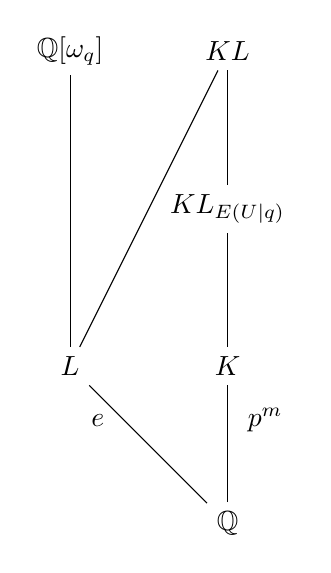
\begin{tikzpicture}
    \node (QBase) at (0,0) {$\Q$};
    \node (QK) at (0,2) {$K$};
    \node (QL) at (-2,2) {$L$};
    \node (QKprime) at (0,4) {$KL_{E(U|q)}$};
    \node (QKL) at (0,6) {$KL$};
    \node (Qwq) at (-2,6) {$\Q[\w_q]$};

    \draw (QBase)--(QK) node [pos=0.7, right,inner sep=0.25cm] {$p^{m}$};
    \draw (QBase)--(QL) node [pos=0.7, left,inner sep=0.25cm] {$e$};
    \draw (QL)--(Qwq);
    \draw (QL)--(QKL);
    \draw (QK)--(QKprime);
    \draw (QKprime)--(QKL);
    \end{tikzpicture}
\]
$K' = KL_{E}$ is the largest field between $K$ and $KL$ in which no primes ramify, so $q$ must be unramified in $K'$.

In $L$, only the prime $q$ is ramifies (it is in fact totally ramified; Exercise 3.24 (a)).  Applying Theorem 31, any prime of $\Q \neq q$ that is not ramified in $K$ is also unramified in $KL$, and so is also unramified in the intermediate subfield $K'$.

\item [31. (d)] TODO - easy
\item [31. (e)] In the direct product $E(Q|q) \times \gal{L}{\Q}$, both sides of the product have cardinality $e$ which is a power of $p$; as $E(Q|q)$ is an injection its cardinality must also be a power of $p$.  Applying Exercise 4.23, we must have $V_1$ trivial ($q$ does not divide a power of $p$).
\item [31. (f)] By (e), $V_1$ is trivial so by Exercise 4.21, $E(U|q)$ is a cyclic group.  TODO: not clear why this shows $E(U|q)$ has cardinality $e$.

\item [31. (g)] We know $e(U|q) = e$.  Since $q$ is totally ramified with degree $e$ in $L$ (31. (b)), $U$ is unramified over $L$.  Conversely, $q$ is unramified in $KL'$ but has total ramification degree of $e$, so $U$ is totally ramified over $KL'$ (definition of inertia field).

\item [31. (h)] $K'L$ Since $U$ is unramified over $L$, $K'L  = KL$ (there can be no intermediate field between $K'$ and $KL$ properly containing $L$ as).  Therefore if $K'$ is contained in a cyclotomic field, so is $K$.  TODO: don't understand this.  TODO: need to know $[K':K]$ to see $[K':\Q]$ a power of $p$.

\item [32.]  We assume $p = 2$; the goal is to show all abelian field extensions of order $p^m$ where only $p$ ramifies are contained in a cyclotomic field.  Since $\gal{K}{\Q}$ is abelian all subgroups correspond to fixed fields under the Galois correspondence.

\item [32. (a)] If $m = 1$, then by Theorem 25 either $2 | m$ or $\modequiv{m}{3}{4}$.  As 2 is the only ramified prime, no prime $p > 2$ can divide $m$ (or else its primes factors would ramify); the only possibilities are $m = \pm 2$ or $m = -1$.  So $K = \Q[\sqrt{2}], \Q[\sqrt{-2}], \Q[i]$.

\item[32. (b)] As $K$ is a field extension of degree $p^m$ it has a nonempty intersection $K \cap \R$ which has degree $p^k$ for $1 < k < m$; by Cauchy's theorem the subgroup of the Galois group associated with $K \cap \R$ has an element of order 2.  The subgroup generated by this element is normal in $\gal{K}{\Q}$ as the extension is Abelian.  The fixed field associated with the element has degree 2 over $\Q$ and is contained in $\R$, therefore it must be $\Q[\sqrt{2}] \subset K$.

\item[32. (c)] Set $L = \R \cap \Q[\w]$ for $\w = e^{2\pi i/2^{m+2}}$.  $L$ is the fixed field of complex conjugation and so has degree $2^{m}$ over $\R$; by Cauchy's Theorem it has an element of order 2 which corresponds to $\Q[\sqrt{2}]$ by 32 (b).  This can be the only quadratic subfield of $L$ as the other possible quadratic extensions have an empty intersection with $\R$.

By the structure theorem on Abelian groups, $L \cong Z_{2^{a_1}} \times \cdots \times Z_{2^{a_k}}$ where $\sum a_i = m$.  However as $L$ has only one subfield of order 2,  $k = 1$; otherwise applying Cauchy's theorem to an element of the direct sum gives different subgroups of order 2.  Therefore $L \cong Z_{2^m}$ and so $L$ is cyclic.

\end{enumerate}

\section*{Chapter 5}

\begin{enumerate}
\item[6.] Show that $\ringofintegers{\Q[\sqrt{m}]}$ is principal for $m = 2, 3, 5, 6, 7, 173, 293, 437$.  As each of these $m$ is positive, these are real quadratic fields and so the number of complex embeddings $s = 0$.  Therefore the bound given by Minkowski's Theorem is that every ideal class contains an ideal with $||J|| < \frac{2!}{2^2} \cdot \sqrt{|\disc{R}|}$, where $\disc{R} = m$ if $\modequiv{m}{1}{4}$ and $\disc{R} = 4m$ otherwise.  Therefore \[ ||J|| < \begin{cases}\frac{\sqrt{m}}{2} &\modequiv{m}{1}{4}\\ \sqrt{m} &\modequiv{m}{2, 3}{4}\end{cases} \]

    \begin{itemize}
        \item[$m = 2$: ] $||J|| < \sqrt{2} \approx 1.4$ so every ideal class contains an ideal with norm 1.  Therefore every ideal must be principal.
        \item[$m = 3$: ] $||J|| < \sqrt{3} \approx 1.7$ so every ideal is principal.
        \item[$m = 5$: ] $||J|| < \sqrt{5} / 2 \approx 1.1$ so every ideal is principal.
        \item[$m = 6$: ] $||J|| < \sqrt{6} \approx 2.4$ so we must check that the prime ideal containing $2$ is principal.  By Theorem 25, 2 factors as $(2, \sqrt{6})^2$ in $\Q[\sqrt{6}]$.  $(2, \sqrt{6})$ is principal, generated by $(2 + \sqrt{6})$: $2 = -1 \cdot (2 + \sqrt{6})(2 - \sqrt{6})$ and $\sqrt{6} = 2 + \sqrt{6} - 2$.  Therefore every ideal is principal.
        \item[$m = 7$: ] $||J|| < \sqrt{7} \approx 2.6$ so we must check that the prime ideal containing $2$ is principal.  By Theorem 25, $2$ factors as $(2, 1 + \sqrt{7})^2$.  $(2, \sqrt{7})$ is generated by $3 + \sqrt{7}$; $2 = (3 + \sqrt{7})(3 - \sqrt{7})$ and $1 + \sqrt{7} = 3 + \sqrt{7} - 2$.  Therefore every ideal is principal.
        \item[$m = 173$: ] $\modequiv{173}{1}{4}$, so $||J|| < \sqrt{173} / 2 \approx 6.5$, so we must check that the prime ideals containing $2, 3, 5$ are all principal.  Since $\modequiv{173}{5}{8}$, $2$ remains prime in $\Q[\sqrt{m}]$ and so its ideal is principal.  173 is a prime number.  Since $\modequiv{173}{1}{4}$, by quadratic reciprocity, $\legendre{173}{p} = \legendre{p}{173}$, so $\legendre{3}{173} = \legendre{173}{3} = \legendre{2}{3} = -1$. Similarly $\legendre{5}{173} = \legendre{173}{5} = \legendre{3}{5} = -1$.  So both 3 and 5 remain inert in $\Q[\sqrt{m}]$ and so every ideal is principal.
        \item[$m = 293$: ] $\modequiv{293}{1}{4}$ so $||J|| < \sqrt{293} / 2 \approx 8.5$ so we must check the prime ideals containing $2, 3, 5, 7$ are all principal.  $\modequiv{293}{5}{8}$ so $2$ remains prime in $\Q[\sqrt{293}]$ and its ideal is principal.  293 is a prime number.  Calculation with Sage shows that $3, 5, 7$ each are not squares mod 293, so these prime ideals remain inert in $\Q[\sqrt{293}]$ and so are principal.  Therefore every ideal is principal.
        \item[$m = 437$: ] $\modequiv{437}{1}{4}$ so $||J|| < \sqrt{437} / 2 \approx 10.4$ so we must check that the prime ideals $2, 3, 5, 7$ are all principal.  $\modequiv{437}{5}{8}$ so $2$ remains prime in $\Q[\sqrt{437}]$.  $437 = 19 \cdot 23$ so none of $3, 5, 7$ ramify in $\sqrt{437}$.  Using Sage we can calculate the Jacobi symbol $\legendre{3, 5, 7}{437} = -1$.  As the Jacobi symbol is -1 each of these are nonresidues mod $437$ and so by Theorem 25 remain prime in $\Q[\sqrt{437}]$.  Therefore every ideal is principal.
    \end{itemize}

\item[10. (a)] For $\Q[\sqrt{m}]$ to be a principal ideal domain, we consider the prime lying over 2.  We enumerate the possibilities:

\begin{itemize}
    \item[$2 \mid m$]: $(2, \sqrt{m})^2 = (2)$; for this to be principal $N(2a + b\sqrt{m}) = 2$; so $4a^2 - b^2 m = 2$.  We must have $a = 0, b = 1, m = -2$.  No other cases where $2 \mid m$ can be principal.
    \item[$\modequiv{m}{3}{4}$]: $(2, 1 + \sqrt{m})^2 = (2)$; for this to be principal it would be generated by an element $2a + b(1 + \sqrt{m})$; the norm of such an element is $4a^2 + 4ab + b^2(1 - m)$.  Setting this equal to 2, we must have $a = 0$ as $m$ is negative; then $b^2 (1-m) = 2$ has 1 solution, $b = 1$, $m = -1$.
    \item[$\modequiv{m}{1}{8}$]: $(2, \frac{1 + \sqrt{m}}{2})(2, \frac{1 - \sqrt{m}}{2}) = (2)$; for this to be principal it would be generated by an element $2a + b(\frac{1 + \sqrt{m}}{2})$.  The norm of such an element is \[ 4a^2 + 2ab + b^2(\frac{1 - m}{4}) \]  Setting this equal to $m$ we again must have $a = 0$; then $b^2(\frac{1 - m}{4}) = 2$; as $\modequiv{m}{1}{8}$ the only solution to this can be $m = -7$.
    \item[$\modequiv{m}{5}{8}$]: $(2)$ remains inert and so remains a principal ideal.
\end{itemize}
Therefore the only possibilities for $\ringofintegers{\Q[\sqrt{m}]}$ to be a PID when $m < 0$ are $\modequiv{m}{5}{8}$, $m = -1$, $m = -2$, $m = -7$.

\item[10. (b)] The problem in the book has a typo (both editions).  The problem statement should be "Suppose $p$ is an odd prime such that $4p < -m$.  Show $m$ is a non-square mod $p$."

    Since $\modequiv{m}{5}{8}$, $\modequiv{m}{1}{4}$.  Let $R = \ringofintegers{\Q[\sqrt{m}]}$.  If $m$ is a square mod $p$, then $pR = (p, \frac{n +\sqrt{m}}{2})(p, \frac{n - \sqrt{m}}{2})$ (by Theorem 25). Suppose $R$ is a PID; therefore the ideal $(p, \frac{n +\sqrt{m}}{2})$ is generated by $\frac{n + \sqrt{m}}{2}$ with $p = (\frac{n +\sqrt{m}}{2})(\frac{n - \sqrt{m}}{2})$.  Therefore \[ n^2 - m = 4p \implies n^2 - m < -m \implies n^2 < 0 \]
    This is a contradicts $\modequiv{n^2}{m}{p}$, so $p$ must be inert in $R$, meaning $m$ is a nonsquare mod $p$.

\item[10. (c)]
    From (a) we know $\modequiv{m}{5}{8}$, and so $\modequiv{m}{1}{4}$.  If $m$ is to be a principal ideal domain, it must be prime: otherwise any prime $p \mid m$ would ramify in $\Q[\sqrt{m}]$ as the ideal $(p, \sqrt{m})$ which is nonprincipal if $\sqrt{m}$ has a norm $\neq p$.

    The first prime above $19$ such that $\modequiv{m}{5}{8}$ is $29$; therefore by (b) any $m < -19$ such that $\ringofintegers{\Q[\sqrt{m}]}$ is a principal ideal domain must have 3, 5, and 7 be inert.

    For an odd prime $p$ to be inert, $m$ must be a non-residue modulo $p$.  We already know that 2 is inert if $\modequiv{m}{5}{8}$.  For 3 to be inert, $\modequiv{m}{2}{3}$.  For 5 to be inert, $\modequiv{m}{\pm 2}{5}$.  For 7 to be inert, $\modequiv{m}{3, 5, 6}{7}$.  Using the Chinese Remainder Theorem on each of these combinations we have \[ \modequiv{m}{-403, -163, -43, -67, -667, -547}{840} \]

    Relevant computation with Sage:
\begin{verbatim}
sage: modulae_list = [([2],3), ([2, 3], 5),
...                   ([3, 5, 6], 7), ([5], 8)]
sage: prime_list = [a[1] for a in modulae_list]
sage: residues = [a[0] for a in modulae_list]
sage: [-(840-CRT_list(list(rs),prime_list))
...    for rs in itertools.product(*residues)]
[-403, -163, -43, -67, -667, -547]
\end{verbatim}
\item[10. (d)] TODO (base off (c))
\item[11.]
    The Minkowski bound for $\Z[\sqrt{-6}]$ is $\frac{2!}{2^2}\left(\frac{4}{\pi}\right)\sqrt{24} \approx 3.11$.  Both 2 and 3 ramify in $\Z[\sqrt{-6}]$ as they divide the discriminant; $(2, \sqrt{-6})^2 = (2)$ and $(3, \sqrt{-6})^2 = (3)$.  Neither of these ideals is principal as $x^2 + 6y^2 = \{2, 3\}$ has no integer solutions. $(2, \sqrt{-6}) = \frac{\sqrt{-6}}{3}(3, \sqrt{-6})$, so they are in the same ideal class element.  Therefore the ideal class group of $\Z[\sqrt{-6}]$ has order 2.

    The Minkowski bound for $\Z[\sqrt{-10}$ is $\frac{2!}{2^2}\left(\frac{4}{\pi}\right)\sqrt{40} \approx 4.02$, so again we only need to consider 2 and 3.  2 ramifies as $(2, \sqrt{-10})^2$; as in the previous case this is not a principal ideal due to $x^2 + 10y^2 = 2$ having no integer solutions.  3 remains inert; $\modequiv{-10}{2}{3}$ and $\legendre{2}{3} = -1$, so 3 does not factor in $\Z[\sqrt{-10}]$.

\item[12.]
    The Minkowski bound for $\Z[\sqrt{-23}]$ is $3.053$, so only 2 and 3 need to be considered.  As $\legendre{2}{-23} = 1$, 2 factors as $2 = \left(2, \frac{\sqrt{-23} - 1}{2}\right)\left(2, \frac{\sqrt{-23} + 1}{2}\right)$.  $x^2 + 23y^2 = 8$ has no integer solutions, so this must be a non-principal ideal.  $\left(2, \frac{\sqrt{-23} - 1}{2}\right)^2 = (4, \sqrt{-23} - 1, \frac{\sqrt{-23} - 11}{2}) = (4, \frac{\sqrt{-23} + 3}{2})$.  This is also not a principal ideal since $x^2 + 23y^2 = 16$ has no solutions with $y \neq 0$ (since $\frac{\sqrt{-23} + 3}{2}$ is in the ideal it can't just be generated by an integer).  However, $\left(2, \frac{\sqrt{-23} - 1}{2}\right)^3 = (8, \sqrt{-23} - 1, \sqrt{-23} + 3, \frac{\sqrt{-23} - 13}{2})$.  First observe $\frac{\sqrt{-23} + 3}{2}$ is in this ideal.  Next, observe $8 = \norm(\frac{\sqrt{-23} + 3}{2})$, so the ideal is principal.  Therefore there are 3 elements in the ideal class group.

    I am (for now) omitting the part of the exercise which asks that we do the same for $-31, -83, -139$.

    (Skip a bunch of quadratic field exercises.)

    \item [17.] Let $\w = e^{2\pi i / 7}$.  $\disc{\Z[\w]} = -7^5$, and $\Z[\w]$ has degree 6 over $\Q$.  There are 6 embeddings from $\Z[\w]$ into $\Q$; each taking $\w$ to a different root of unit.  Therefore the Minkowski bound is $\frac{6!}{6^6}\left((\frac{4}{\pi}\right)^{3}\sqrt{7^5} = \frac{720 \cdot 64 \cdot 49\sqrt{7}}{\pi^3 6^6} = \frac{3920\sqrt{7}}{81\pi^3} \approx 4.12$.  So the only prime ideals we need to examine contain 2 or 3.

    By the Corollary to Theorem 26, $2$ splits into $\frac{\varphi(7)}{3} = 2$ ideals mod 7 ($\modequiv{2^3}{1}{7}$, while $3$ remains inert.  Mod 2, $x^6 + x^5 + x^4 + x^3 + x^2 + x + 1$ factors as $(x^3 + x + 1)(x^3 + x^2 + 1)$, so $2 = (2, \w^3 + \w + 1)(2, \w^3 + \w^2 + 1)$.  As $(\w^3 + \w + 1)(\w^3 + \w^2 + 1)(\w^4) = 2$, so both of these ideals is principal.  Therefore $\Z[\w]$ is a PID.

    Next, let $\Z[\w + \w^{-1}]$.  By Exercise 2.35, the discriminant over this number field is $7^{2} = 49$.  This is a real subfield of order 3 over $\Q$ (no embeddings in $\C$) so its Minkowski bound is $\frac{3!}{3^3}{\sqrt(49)} = \frac{14}{9} < 2$, so $\Z[\w + \w^{-1}]$ is a PID.

    \item[18.] Let $\w = e^{2\pi i / 11}$.
    This is a real subfield of degree 5 over $\Q$ with discriminant $11^{4}$, so its Minkowski bound is $\frac{5!}{5^5}\cdot 11^2 = \frac{2904}{625} \approx 4.6$.  So we must investigate the prime ideals 2 and 3.

    By Exercise 4.12, primes in $\Z[\z_{p} + \z_{p}^{-1}]$ for $\z_{p}$ a $p$th root of unity split into $\frac{p - 1}{2f}$ ideals, where $f$ the smallest integer so that $\modequiv{p^f}{\pm 1}{p}$.  Letting $p = 11$ and looking at 2 and 3, we have both $\modequiv{2^5}{-1}{11}$ and $\modequiv{3^5}{1}{11}$, so both 2 and 3 remain inert in $\Z[\w]$.  Therefore $\Z[\w]$ is a PID.

    We repeat the same process for $\w = e^{2\pi i / 13}$.  In this case the discriminant of $\Z[\w + \w^{-1}] = 13^{5}$ so the Minkowski bound is $\frac{6! 169 \sqrt{13}}{6^6} = \frac{845\sqrt{13}}{324} \approx 9.403$.  We must examine the primes 2, 3, 5, 7.  Here the ideal splitting formula that a prime splits into $\frac{6}{f}$ ideals.

    $2$ and $7$ remain inert in $\Z[\w + \w^{-1}]$ ($\modequiv{2^6, 7^6}{-1}{13}$), but $3$ splits into 2 ideals ($\modequiv{3^3}{1}{13}$) and $5$ splits into 3 ideals ($\modequiv{5^2}{-1}{13}$).  Computation via Sage shows each of these ideals is principal.  Therefore $\Z[\w + \w^{-1}]$ is a PID.

    \item [19.]

    Let $K = \Q[\sqrt[3]{2}]$.  $\ringofintegers{K} = \Z[\sqrt[3]{2}]$ by Exercise 41 of Chapter 2 ($\modnotequiv{2}{\pm 1}{9}$), and $\disc{\Z[\sqrt[3]{2}]} = -27(2)^2$.  There are 2 complex embeddings for $K$ so the Minkowski bound of $K$ is $\frac{3!}{3^3}\left(\frac{4}{\pi}\right)\sqrt{|-27 \cdot 2^2|} = \frac{16\sqrt{3}}{3\pi} \approx 2.94$.  The only prime ideal class we must investigate is the one lying over $(2)$; however, 2 is fully ramified in $\ringofintegers{A}{K}$, and so its ideal is $(2, \sqrt[3]{2})^3 = (\sqrt[3]{2})^3$ is principal.  Therefore $\Z[\sqrt[3]{2}]$ is a PID.

    Let $\alpha$ be a root of $\alpha^3 - \alpha - 1$.  By Exercise 2.28 $\ringofintegers{\Q[\alpha]} = \Z[\alpha]$, and $\disc{\alpha} = -(-4 + 27) = -23$.  This field also has 2 complex embeddings (there is only 1 real root), so the Minkowski bound is $\frac{8\sqrt{23}}{9\pi} \approx 1.356$.  There are no primes within this bound so every ideal of $\Z[\alpha]$ is a principal ideal.

    \item [20.] Let $\alpha$ be a root of $\alpha^3 - \alpha - 7$.  By Exercise 2.28, $\disc{\alpha} = (-4 + 27 \cdot 7^2) = -1319$.  This is prime (so squarefree) and so $\ringofintegers{\Q[\alpha]} = \Z[\alpha]$ by Exercise 2.27.  This field has 2 complex embeddings (only 1 real real root) so the Minkowski bound is $\frac{8\sqrt{1319}}{9\pi} \approx 10.27$.  We must investigate the primes 2, 3, 5, and 7.  Since $\disc{\alpha}$ is prime each of these factors in the Dedekind way, e.g. by seeing how the polynomial $\alpha^3 - \alpha - 7$ factors mod $p$.  Additionally, since the minimum polynomial has degree 3 the prime remains inert if there is no root mod $p$.

    \begin{itemize}
        \item $p = 2: \modequiv{x^3 - x - 7}{x^3 + x + 1}{2}$.  This has a root if there is an $x$ so that $x(x^2 + 1) = 1$ (clearly not), so 2 remains inert.
        \item $p = 3: \modequiv{x^3 - x - 7}{x^3 + 2x + 2}{3}$.  This has a root if $x(x^2 + 2) = 1$; however no options work.  3 remains inert.
        \item $p = 5: \modequiv{x^3 - x - 7}{x^3 + 4x + 3}{3}$.  This has a root if $x(x^2 + 4) = 2$; again no options work.
        \item $p = 7$: as per the hint, $7 = \alpha^3 - \alpha = \alpha(\alpha + 1)(\alpha - 1)$, so $(7) = (7, \alpha)(7, \alpha + 1)(7, \alpha - 1)$.  Since $\norm(\alpha) = 7$ it is a principal ideal.  $\alpha + 1$ is the root of the polynomial $x^3 - 3x^2 + 2x - 7$ (determined via Sage) so $\norm(\alpha + 1) = 7$ and $(\alpha + 1)$ is also principal.  Similarly $\norm(\alpha - 1) = 7$ and so $(7, \alpha - 1)$ is principal.
    \end{itemize}

    We have considered all ideals below the Minkowski bound; each of these are principal, so $\Z[\alpha]$ must be a PID.

    \item [21.] By the binomial theorem, $(\sqrt[3]{m} + a)^3 = m + 3a(\sqrt[3]{m})^2 + 3a^2(\sqrt[3]{m}) + a^3$.  Therefore the minimum polynomial for $\sqrt[3]{m} + a$ is $x^3 - \text{something}\cdot x^2 - \text{something} \cdot x - (m + a^3)$, so $\norm(\sqrt[3]{m} + a) = m + a^3$.

    \item [22.] Any purely cubic field has 2 complex embeddings, so the Minkowski bound is $\frac{3!}{3^3}\left(\frac{4}{\pi}\right)\sqrt{|-27m^2|}$ = $\frac{8m\sqrt{3}}{3\pi}$.  By Exercise 2.41, if $\modnotequiv{m}{\pm 1}{9}$,  $\ringofintegers{K} = \Z[\sqrt[3]{m}]$ (this is the case for $m = 3, 5, 6$).  A real cubic field has degree 3 over $\Q$, so it has no non-trivial subfields and if a prime ramifies, it is totally ramified.

    $m = 3$: the Minkowski bound is $\approx 4.4$ and 3 ramifies as $(\sqrt[3]{3})^3$ (principal).  $(\sqrt[3]{3}^2 + \sqrt[3]{3} + 1)(\sqrt[3]{3} - 1) = (2)$; by Exercise 21, $\norm(\sqrt[3]{3} - 1) = 3 + (-1)^3 = 2$ and so both the ideals lying over 2 are principal.  Therefore $\Q[\sqrt[3]{3}]$ is a PID.

    $m = 5$: the Minkowski bound is $\approx 7.3$.  Since $5$ ramifies as $(\sqrt[3]{5})^3$ (principal) we need to examine the ideal classes of 2, 3, and 7.  Let $\alpha = \sqrt[3]{5}$.

    The polynomial $\modequiv{x^3 - 5}{x^3 + 1}{2}$ factors as $(x + 1)(x^2 + x + 1)$, so by Dedekind factoring (Theorem 25) 2 splits into two factors, $(2, \alpha + 1)(2, \alpha^2 + \alpha + 1)$.  Sage indicates that these are principal ideals and equal to $(\alpha^2 - \alpha - 1)(\alpha^2 + 2\alpha + 3)$.  [Not sure how to see this without a computer algebra program]

    $\alpha - 2$ has norm $-3$ and so the ideal $(\alpha - 2)$ that lies over 3 is principal (in fact this ideal ramifies over 3).

    Considering the ideal class of $(7)$: $x^3 - 5$ is irreducible mod 7; if it were reducible it would have a root, but 5 is not a cubic residue mod 7.  Therefore 7 remains inert.  Therefore $\Q[\sqrt[3]{5}]$ is a PID.

    $m = 6$: the Minkowski bound is $\approx 8.8$, so we again must consider the ideal class groups of 2, 3, 5, and 7.  Let $\alpha = \sqrt[3]{6}$.

    By Exercise 21, $\norm(\alpha - 2) = -2$; as 2 is ramified, 2 factors as $(\alpha - 2)^3$.  3, 5, and 7 are seen as principal via Sage computation.  $3$ is ramified as $(\alpha^2 + 2\alpha +3)^3$, $5$ has the principal ideals $(\alpha -1)$ and $(\alpha^2 + \alpha + 1)$ both with norm $5$ lying over it, and 7 factors as $(7) = (\alpha + 1)(2\alpha^2 + 4\alpha + 7)(\alpha^2 + \alpha - 5)$.  Therefore $\Z[\alpha]$ is a PID.

    \item[23. (a)] We let $K = \Q[\sqrt[3]{m}]$ and take $\alpha = \sqrt[3]{m}$.  By Exercise 2.17, the norm of $\alpha + b\alpha + c\alpha^2$ is the determinant of multiplying this element by each of the $K$ basis $\{1, \alpha, \alpha^2\}$.  Therefore:
    \[
        \norm(a + b\alpha + c\alpha^2)\ =\det\left(
        \begin{matrix}
            a & cm &bm \\
            b & a & cm \\
            c & b & a
        \end{matrix}\right) = a^3 + c^3 m^2 + b^3 m - 3abcm
    \]
    \item[23. (b)] If $m$ is squarefree then there are two possiblities based on whether or not $m \equiv \pm 1\ (9)$.

    If $m \not\equiv \pm 1\ (9)$, then $\{1, \alpha, \alpha^2\}$ is an integral basis (Exercise 2.41).  Any $\beta \in \ringofintegers{K}$ has the form $\beta$ has the form $a + b\alpha  + c\alpha^2$ and so by $(a)$, $\modequiv{\norm(\beta)}{a^3}{m}$.

    If $m \equiv \pm 1\ (9)$, then $\left\{1, \alpha, \frac{\alpha^2 \pm \alpha + 1}{3}\right\}$ is an integral basis (Exercise 2.41).  Therefore \[\ringofintegers{K} = \left\{\frac{a \pm b\alpha + c\alpha^2}{3}\ |\ a \equiv b \equiv c \ (3) \right\}\]  Since $m \equiv \pm 1\ (9)$, 3 has an inverse mod $m$. and so $\norm(\frac{a \pm b\alpha + c\alpha^2}{3}) \equiv (3^{-1})^3 \norm(a \pm b\alpha + c\alpha^2)\ (m)$.  By (a), $\norm(a \pm b\alpha + c\alpha^2)$ is a cube mod $m$ and so $\beta$ is a cube mod $m$.

    \item[24.]  Let $K = \Z[\sqrt[3]{7}]$ and $\alpha = \sqrt[3]{7}$.  The Minkowski bound $\approx 10.29$ so we must examine the ideals $(2), (3), (5), (7)$.  $(7)$ ramifies as the principal ideal $(\alpha)^3 = 7$.  $(2)$ and $(5)$ factor as per Dedekind.

    $\modequiv{x^3 - 7}{x^3 + 1}{2}$ so mod 2, $(2) = (2, \alpha + 1)(2, \alpha^2 + \alpha + 1)$.  By Exercise 23, $\norm(\alpha + 1) = 1 + 7 = 8$, so $(2, \alpha + 1)$ is not principal.  Similarly, $\norm(\alpha^2 + \alpha + 1) = 1 + 7^2 + 7 - 21 = 36$, and so $(2, \alpha^2 + \alpha + 1)$ is also not principal.  $(2, \alpha + 1)^2 = (4, 2\alpha+2, \alpha^2 + 2\alpha + 1) = (4, \alpha + 1)$.  $(2, \alpha + 1)^3 = (\alpha + 1)$ which is principal.  There are thus at least 3 ideal classes.

    $x^3 - 7 \equiv x^3 + 3 \equiv (x - 3)(x^2 + 3x+ 4)\ (5)$, so $(5) = (5, \alpha - 3)(5, \alpha^2 + 3\alpha + 4)$.  Examining norms shows neither of these ideals is principal (the method used is the same as for the case mod 2; $\norm(\alpha - 3) = \norm(\alpha + 2) = 7 + 2^3 = 8$, $\norm(\alpha^2 + 3\alpha + 4) = 4^3 + 7 \cdot 3^3 + 7^2 - 3 \cdot 7 \cdot 12 = 50$).  Calculation with Sage shows $(5, \alpha - 3) \cdot (\alpha + 1) = (2, \alpha + 1) \cdot (\alpha - 3) = (40, \alpha + 17)$ so these two ideals are in the same ideal class.  As these two ideals are in the same ideal class their inverses must also be.  Therefore there are three ideal classes in $\Z[\sqrt[3]{7}]$.

    \item[25. (a)] Letting $R = \ringofintegers{\Q[\sqrt[3]{x}]}$ we look for elements with norm 3; The factor of $1/3$ gives a multiplicative $1/27$ factor for the norm.  From Exercise 5.23 we are looking for $a, b, c$ where
    \[ a^3 + 17b^3 + 289c^3 - 51abc = 81 \]
    Setting $a = 4$, $c = 1$ reduces to
    \[ 17b^3 - 285b^3 = -272 = -17 \cdot 16 \]
    and so \[ b^3 - 12b + 16 = 0 \]
    This has two solutions; $b = 2$ and $b = -4$; both of these are compatible with $a \equiv -b \equiv c\ (3)$.  So we have two elements
    \[ \beta = \frac{4 + 2\alpha + \alpha^3}{3} \]
    \[ \gamma = \frac{4 - 4\alpha + \alpha^3}{3} \]
    Sage confirms $\gcd(\beta, \gamma) = 1$  (not clear how to see this by hand)
    Since $\gcd(\beta, \gamma) = 1$ and $\norm(\beta) = \norm(\gamma) = 3$, $(\beta)$ and $(\gamma)$ are prime ideals lying over 3 in $K$.

    \item [25. (b)] The Minkowski bound for $K$ is $\frac{3!}{27}\left ( \frac{4}{\pi}\right){\sqrt{|-867|}} \approx 8.3$ so we must investigate how the primes $2, 3, 5, 7$ factor. $|K / R[\alpha]| = 3$ so $2, 5, 7$ factor as per Dedekind (also follows from Exercise 3.26 (a)).

    We begin with $p = 2$.  $x^3 - 17 \equiv x^3 + 1\ (2)$ which factors as $(x^2 + x + 1)(x + 1)$; therefore $2R = (2, \alpha^2 + \alpha + 1)(2, \alpha + 1)$.  We focus on $\alpha + 1$.  By Exercise 5.21, $\norm(\alpha + 1) = 17 + 1 = 18$, so if this is a principal ideal, then $(\alpha + 1) = (\text{element with norm 9})(\text{element with norm 2})$.  Looking around for an element with norm 9, we see that $\norm(\alpha - 2) = 17 - 8 = 9$, so $\norm\left(\frac{\alpha + 1}{\alpha - 2}\right) = 2$.  Using a computer algebra system we see that \[ \frac{\alpha + 1}{\alpha - 2} = \frac{\alpha^2 + 2\alpha + 7}{3} \]  Therefore $(2, \alpha + 1)$ is thus principal, generated by this element.  As one of the prime ideals over 2 is principal, the other ideal $(2, \alpha^2 + \alpha + 1)$ must also be principal.

    For $p = 5$, $x^3 - 17 \equiv x^3 + 1\ (2)$ which factors as $(x^2 + 3x + 4)(x + 2)$ and so $5R = (5, \alpha^2 + 3\alpha + 4)(5, \alpha + 2)$.  As before we focus on the factor with a linear factor (our goal is to find an element with norm 5 to make $(5, \alpha + 2)$ principal); $\alpha - 3 \in (5, \alpha + 2)$ and $\norm(\alpha - 3) = 17 - 27 = - 10$.  We already found an element of norm 2 for $p = 2$; in dividing $\alpha - 3$ by $\frac{-\alpha^2 - 2\alpha - 7}{3}$ in a computer algebra system, we see the element $\frac{-2\alpha^2 - \alpha + 16}{3}$ has norm 5 and so must generate $(5, \alpha + 2)$.  As in the $p = 2$ case, since one of the prime ideals lying over 5 is principal, the other must be as well.

    For $p = 7$ the polynomial $x^3 - 17$ has no root mod 7 and so is irreducible.  Therefore the prime 7 of $\Z$ stays inert in $R$.

    We have checked the factoring for all the primes within the Minkowski bound and they all either stay inert or factor into principal ideals; therefore $R$ is a principal ideal domain.

    \item[26.] This problem investigates $K = \Q[\sqrt[3]{19}]$ and \[ R = \ringofintegers{K} = \left\{\frac{a + b\alpha + c\alpha^3}{3}\ |\ a \equiv b \equiv c\ (3)\right\} \]
    The Minkowski bound is just a little larger than in 25 ($\approx 9.3$) and so the key primes we must consider are the same: 2, 3, 5, 7.  As before 3 ramifies and the other primes can be factored as per the Dedekind method.

    We have the following factorizations:
    \begin{eqnarray*}
        2R &=& (2, \alpha + 1)(2, \alpha^2 + \alpha + 1) \\
        3R &=& P^2Q \text{ (per Exercise 3.26e)}\\
        5R &=& (5, \alpha + 1)(5, \alpha^2 + 4\alpha + 1) \\
        7R &=& \text{remains inert}
    \end{eqnarray*}

    By Exercise 5.22(b), $\norm(\beta)$ is a cube mod $19$ for all $\beta \in R$; however $2, 3, 5$ are each cubic non-residues.  Therefore there are no elements in $R$ with these norms, so the prime ideals of $R$ lying over these ideals in $\Z$ are non-principal.

    \item[26. (a)]  First note that the primes over 3 are generated by $P$, as $P^2 Q = e$, $Q^{-1} = P^2$ and so $Q = (P^{-1})^2 = P^{n-2}$, letting $n$ be the size of the ideal class group.

    We next find elements with norm divisible by 2, 3, and 5.  $\norm(\alpha - 1) = 18 = 3^2 \cdot 2$ and so either $P$, $Q$ (or both) lie over the ideal $(\alpha - 1)$; as $\bar{Q}$ is some power of $P$ we can write $(\alpha - 1) = P^m I$ where $||I|| = 2$ and $I$ is a prime ideal over 2; then $I = P^{n - m}$.  As $I$ is a power of $P$ its inverse must be as well.

    Similarly $4 - \alpha \in (5, \alpha + 1)$ with $\norm(4 - \alpha) = 45 = 3^2 \cdot 5$ and so $(4 - \alpha) = P^{k} J$ where $||J|| = 5$ and $J$ is a prime lying over 5.  Similarly $J = P^{n - k}$.

    We have investigated all ideals less than the Minkowski bound and so the ideal class group must be cyclic, generated by the class containing $P$.

    \item[26. (b)] $\norm(\alpha + 2) = 27$ (TODO)

    %  the subgroup $\{P^2, Q, e\}$ has order 3 and so by Lagrange's Theorem, $3 \mid n$ for $n$ the size of the ideal class group.
    % Could $P^2 = Q$?

    \item [35.] Let $K$ be a cubic extension of $\Q$ with 1 embedding in $\R$, and take $u$ to be the fundamental unit of $R = \ringofintegers{K}$. Thus $u > 1$ and (as $R$ contains no roots of unity aside from $\pm 1$) all units in $R$ have the form $\pm u^{k}$, $k \in \Z$.  Our goal is to find a lower bound for $u$.

    \item [35. (a)] Let $u$, $\rho e^{i\theta}$, $\rho e^{-i\theta}$ be the conjugates of $u$.  Show $u = \rho^{-2}$ and obtain a formula for $\disc{u}$.

    Since $u$ is a unit, the product of all its conjugates is equal to 1, so $u \rho^2 e^{i\theta} e^{-i\theta} = u\rho^2 = 1$, so $u = \rho^{-2}$.

    By applying Theorem 8, we have
    \[
    \disc{u} = (u - \rho e^{i\theta})^2 (u - \rho e^{-i\theta})^2 (\rho e^{i\theta} - \rho e^{-i\theta})^2
    \]

    Recalling Euler's formula ($e^{i\theta} = \cos{\theta} + i\sin{\theta}$), $e^{i\theta} - e^{-i\theta} = 2i \sin{\theta}$ and $e^{i\theta} + e^{-i\theta} = 2\cos{\theta}$

    Replacing $u$ with $\p^{-2}$ we simplify the discriminant formula to:

    \begin{eqnarray*}
        \disc{u} &=& (\rho^{-2} - \rho e^{i\theta})^2 (\rho^{-2} - \rho e^{-i\theta})^2 (-4\rho^2 \sin^2{\theta}) \\
                 &=& -4\sin^2{\theta} \cdot \rho^{6} \cdot [(\rho^{-3} - e^{i\theta})(\rho^{-3} - e^{-i\theta})]^2 \\
                 &=& -4\sin^2{\theta} \cdot \rho^{6} \cdot [(\rho^{-6} - \rho^{-3}(e^{i\theta} + e^{-i\theta}) + 1)]^2 \\
                 &=& -4\sin^2{\theta} \cdot \rho^{6} \cdot [(\rho^{-6} - \rho^{-3}(2 \cos {\theta}) + 1)]^2 \\
                 &=& -4\sin^2{\theta} (\rho^{-3} - 2 \cos {\theta} + \rho^{3})^2
    \end{eqnarray*}

    This is the required result.

    \item [35. (b)] We obtain an upper bound on $|\disc{u}|$ following the book's suggested method.  Let $x = \rho^{3} + \rho^{-3}$ ($x$ is just an arbitrary variable), fix $c = \cos{\theta}$; we find the maximum value of $f(x) = (1 - c^2)(x - 2c)^2 - x^2$.  The idea is to bound $|disc(u)|$ by $(\rho^3 + \rho^{-3} + k)$ for some constant $k$; $u = \rho^{-2}$ and $u > 1$ so this will give us an effective bound.

    Letting $f(x)$ be as above, we observe $f$ is an negatively oriented parabola; as $1 - c^2 < 1$, the $-x^2$ term dominates.  We take its derivative: $f'(x) = (1 - c^2)(2x - 4c) - 2x = -c^2 \cdot 2x - (1 -c^2)4c$.  This obtains a maximum value at $x = 2(1-c^2) / c = -\frac{2}{c} + 2c$; plugging this value back into $f$, we see the maximum value of \[ f_{max} = (1 - c^2)\frac{4}{c^2} - {\frac{4}{c^2} - 8 + 4c^2} =  4 - 4c^2 = 4(1 - c^2) \]

    Thus the maximum differential between the "accurate" formula for $\disc{u}$ and its quadratic approximation is at most 4, so $|\disc{u}| < 4((p^{3} + p^{-3})^2 + 4)  = 4(p^6 + p^{-6} + 6) = 4(u^{-3} + u^{3} + 6)$ giving the required bound.

    \item [35. (c)] Letting $d = |\disc{R}|$, $d \le \disc{u}$, thus $d \le \disc{u} < 4(u^3 + u^{-3} + 6) \implies d/4 < u^{3} + u^{-3} + 6 \implies u^{3} > d/4 - 6 - u^{-3}$.  As $u > 1$, $u^{-3} < 1$ and so $u^{3} > d/4 - 7$.

    \item [35. (d)] TODO

    \item [36.] Let $\alpha = \sqrt[3]{2}$; then $\ringofintegers{\Q[\alpha]} = \Z[\alpha]$ and $\disc{\alpha} = -108$ by Exercise 2.41.
    \item [36. (a)] Using the bound from Exercise 5.35, $u^3 > 81 / 4 > 20$.
    \item [36. (b)] Letting $\beta = (\alpha^2 + \alpha + 1)$, then $\beta(\alpha - 1) = 1$ and so $\beta = \alpha^{-1}$.  As $\alpha \approx 1.2$, $\beta = \alpha^2 + \alpha + 1 \approx 3.8$.  If $u^3 > 20$, $u^2 > 20^{2/3} \approx 7.3$, thus $\beta$ is a unit between 1 and $u^2$ and so $\beta$ is the fundamental unit of $R$.
    \item [37. (a)] If $\alpha$ is the root of a monic polynomial $f$ over $\Z$ and $f(r) = \pm 1$, then $\alpha - r$ is the root of the polynomial $g(x) = f(x + r)$.  \[ g(x) = (x + r)^n + \cdots a_1(x + r) + a_0 = \text{stuff} + r^n + \cdots a_1 r + a_0 = \text{stuff} + f(r) \] Therefore $g$ has constant term $\pm 1$; $\alpha - r$ is a root of $g$ so $\alpha - r$ is a unit.

    \item [37. (b)] Letting $\alpha = \sqrt[3]{7}$; by Exercise 2.41, $\ringofintegers{\Q[\alpha]} = \Z[\alpha]$.  Using part (a), $2 - \alpha$ is a unit; however it is $ < 1$ as $\sqrt[3]{7} \approx 1.91$.  $\beta = (2 - \alpha)^{-1} = \alpha^2 +2\alpha + 4$ (this can be seen through computer algebra systems like Sage or through multiplying out $(2 - \alpha)(a\alpha^2 + b\alpha + c) = 1$ and solving for $a, b, c$).  $\alpha^2 + 2\alpha + 4 \approx 11.485$; however $\disc{\alpha} = -3^3 \cdot 7^2 = -1323$ and so the bound for Exercise 5.35 gives $u^3 > 324$ and so $u^2 > 47.173$; therefore $\beta$ is a unit between 1 and $u^2$ and so must be the fundamental unit of $R$.

    \item [37. (c)] Letting $\alpha = \sqrt[3]{3}$; by Exercise 2.41, $\ringofintegers{\Q[\alpha]} = \Z[\alpha]$.  Using the suggestion, we know that $\alpha^2$ is a root of the polynomial $f(x) = x^3 - 9$; therefore $\alpha^2  - 2$ is a unit by (a).  $\beta = (\alpha^2 - 2)^{-1} = 2\alpha^2 + 3\alpha + 4$ (again through Sage or through solving a system of equations); $beta \approx 12.486$.  $\disc{\alpha} = -27 \cdot 3^2 = 243$ so the bound for Exercise 5.35 gives $u^3 > (243 - 27) / 4 = 54$ and $u^2 > (54)^(2/3) \approx 14.286$; therefore $\beta$ is a unit between 1 and $u^2$ and so must be the fundamental unit of $R$.

    \item [38. (a)] Taking $f(x) = x^3 + x - 3$; $f'(x) = 3x^2 + 1$ has no points on the real line where $f'(x) = 0$ and so $f$ is thus monotonically increasing over $\R$ and so has only one real zero.  $f(1.2) = 1.2^3 + 1.2 - 3 = 2.928 - 3 < 0$ and so $\alpha$ the root of $f$ must be $ > 1.2$.  (Sage gives $\alpha \approx 1.213$).
    \item [38. (b)] By Exercise 2.28, $\disc{\alpha} = -(4 + 27\cdot 3^2) = 247 = 13 \cdot 19$; as its discriminant is squarefree, $\ringofintegers{\Q[\alpha]} = \Z[\alpha]$.
    \item [38. (c)] $f(1) = -1$ so we can apply Exercise 5.37 to see that $\alpha - 1$ is a unit; however it is $< 1$ and so we focus on $\beta = (\alpha - 1)^{-1} = \alpha^2 + \alpha + 2 \approx 4.64$.  The bound from Exercise 5.35 gives $u^3 > (247 - 27)/4 = 55$ so $u^2 > (55)^{2/3} \approx 14.46$; thus $\beta$ is a unit of $R$ between $1$ and $u^2$ and so is the fundamental unit of $R$.

    \item [39.] Let $\alpha^3 = 2\alpha + 3$; thus $\alpha$ is a root of the polynomial $f(x) = x^3 - 2x - 3$.  $f'(x) = 3x^2 - 2$ which takes on zero values at $\pm \sqrt{2/3}$.  Its graph of $f(x)$ increases until $x = -\sqrt{2/3}$ where $f(x) = -(2/3)^{3/2} + 2\sqrt{2/3} - 3 \approx -1.91$ and then it decreases until $x = \sqrt{2/3}$ (where $f(x) \approx -4.08$) after which it monotonically increases for the rest of its range and so crossing the $y$ axis only once (1 real root).  $f(1.9) \approx 0.0059$ and so $\alpha < 1.9$.

    By Exercise 2.28, $\disc{\alpha} = -(4 \cdot (-2)^3 + 27\cdot 3^2) = (-32 + 27 \cdot 9) = -211$; 211 is prime so $\ringofintegers{\Q[\alpha]} = \Z[\alpha]$.  $f(2) = 1$ so $2 - \alpha$ is a unit by 5.37, again we focus on $\beta = (2 - \alpha)^{-1} = \alpha^2 + 2\alpha + 2 \approx 9.41$.  Our bound from Exercise 5.35 is $u^3 > (211 - 27)/4 = 46$ so $ u^2 > (46)^(2/3) \approx 12.838$. $\beta$ is thus a unit between 1 and $u^2$ and so is the fundamental unit of $R$.

    \item[40.] In this problem we will investigate cubic fields given by the polynomial $f(x) = x^3 + ax - 1$.
    \item[40. (a)] Given $a > 0$, we show $x^3 + ax - 1$ is irreducible over $\Q$ by showing it is irreducible over $\Z$ (Gauss's Lemma).  If $f(x)$ is reducible it has the form $f(x) = (x - r)g(x)$ where $g(x)$ has degree 2.  However $r$ would be need to be a divisor of the constant term of $f(x)$ (1) but the only divisors of 1 are $\pm 1$; $f(1) = a \neq 0$ and $f(-1) = -(2 + a) \neq 0$ so $f(x)$ is irreducible.

    $f'(x) = 3x^2 + a$; as $a > 0$, $f'(x)$ has no zeros and so is monotonically increasing; therefore it has only 1 real root.  Additionally $f(0) = -1$ and $f(1) = a$ so its root $0 < \alpha < 1$.

    Note $\alpha$ is a unit as it is the root of a monic polynomial with constant term $-1$.  Additionally $\alpha^{-1} = \alpha^2 + a$: \[ \alpha(\alpha^2 + a) = \alpha^3 + a\alpha = -(a\alpha - 1) + a\alpha = 1 \]

    \item [40. (b)] By Exercise 2.28, $\disc{\alpha} = -(4a^3 + 27\cdot 1^2) = -(4a^3 + 27)$.
    \item [40. (c)] If $4a^3 + 27$ is squarefree, then $\ringofintegers{\Q[\alpha]} = \Z[\alpha]$.  By the above, $\alpha^{-1} = \alpha^2 + a$; since $\alpha < 1$, $a < \alpha^{-1} < a + 1$.  The bound from Exercise 5.35 gives $u^3 > a^3$ and so $u^2 > a^2$; $\alpha^{-1} < a^2 < u^2$ for $a \ge 2$ (when $a = 1$, $a + 1 = 2 \not< a^2 = 1$), thus $\alpha^{-1}$ is the fundamental unit when $a \ge 2$ and $4a^3 + 27$ is squarefree.
    \item [40. (d)] Let $m$ be the squarefree part of $4a^3 + 27$ ($4a^3 + 27 = k^2 m$, $m$ squarefree).  Show if $(m - 27)^2 \ge 16(a+ 1)^3$ then $\alpha^{-1} = \alpha^2 + a$ is the fundamental unit $u$.

    The necessary condition is $\alpha^{-1} < a + 1 < u^2$; the bound from Exercise 35 gives $u^2 > [(m - 27)/4]^(2/3)$. Combining these bounds and clearing denominators gives $16(a + 1)^3 \le (m - 27)^3 < u^2$; if this holds then $\alpha^{-1} < u^2$ and so $\alpha^{-1} = u$.

    We use Sage to check this for $a, 2 \le a \le 25$.
    \begin{verbatim}
sage: for a in range(2, 26):
....:     d = (4*a^3 + 27)
....:     if is_squarefree(d):
....:         continue
....:     m = squarefree_part(d)
....:     bound = (m - 27)**2 >= 16*(a + 3)^3
....:     if not bound:
....:         print(a)
....:
3
6
8
15
    \end{verbatim}
    Therefore the exceptional cases are 3, 6, 8, 15.
    \item[40. (e)] When $a = 8$, $\disc{\alpha} = 4\cdot8^3 + 27 = 2075 = 5^2 \cdot 83$, so the bound from Exercise 5.35 gives $u^3 > (83 - 27)/4 = 14$.  So $u^2 > 5.808$; therefore $\beta = \alpha^{-1}$ is a unit $\beta < u^3$ so it is either $u$ or $u^2$.

    When $a = 15, \disc{\alpha} = 4\cdot 15^3 + 27 = 13527 = 3^4 \cdot 167$; the bound from Exercise 5.35 gives $u^3 > (167 - 27) / 4 = 35$.  So $u^2 > 10.699$; therefore $\beta = \alpha^{-1}$ is a unit $\beta < u^3$ so it must be either $u$ or $u^2$.

    \item[40. (f)] We recall that from Exercise 3.29, there is a homomorphism from $R$ to $\Z_p$ which maps roots $\alpha$ of $f(x)$ to roots of $f(x)$ interpreted as a polynomial over $\Z_p$, assuming $p \not\mid |R/\Z[\alpha]|$.  We take $a = 15$; $\disc{\alpha} = 3^4 \cdot 167$ (so $|R/\Z[\alpha]| \in {1, 3}$).  $f(2) = 37$ which is a prime number so $\psi : R \to \Z_{37}$ is a homomorphism of rings; however 2 is a quadratic non-residue mod 37; therefore $\alpha$ is a non-square in $R$.  Therefore, $\alpha^{-1} = \alpha^2 + 15$ is also a non-square and so $\alpha^{-1}$ is the fundamental unit of $R$.

    \item[40. (g)]
    \begin{eqnarray*}
        (\alpha^2 - 2\alpha + 2)^2 &=& \alpha^4 - 4\alpha^3 + 8 \alpha^2 - 8 \alpha + 4 \\
                                   &=& \alpha(\alpha^3 - 4\alpha^2) + 8 \alpha^2 - 8 \alpha + 4 \\
                                   &=& \alpha(1- 8 \alpha - 4\alpha^2) +  8 \alpha^2 - 8 \alpha + 4\\
                                   &=& \alpha - 4\alpha^3 - 8 \alpha + 4\\
                                   &=& \alpha - 4(1 - 8\alpha) - 8 \alpha + 4\\
                                   &=& 32\alpha - 8\alpha + \alpha = 25\alpha
    \end{eqnarray*}
    Therefore a reasonable guess would be $\left(\frac{\alpha^2 - 2\alpha + 2}{5}\right)^2 = \alpha$; Sage confirms this element is a member of $R$.  (Not clear how best to see this manually; doing the integral basis calculation by hand seems quite annoying.)  Therefore $\beta = \alpha^{-1}$ is a square as well (and so is $u^2$); Sage gives it as $\beta = \left(\frac{2\alpha^2 + \alpha + 14}{5}\right)^2$; this is the fundamental unit of $R$.

    \item[41.] This problem concerns the polynomial $f(x) = x^3 + ax - a$ when $f$ has only 1 real root.
    \item[41. (a)] The case where $a = 1$ reduces to Exercise 40 ($f$ is irreducible using Gauss's lemma); otherwise $f(x)$ is seen to be irreducible using the Eisenstein criterion with any prime divisor of $a$.

    When $a > 0$, $f'(x) = 3x^2 + a$ which has no real zeros; therefore $f$ is monotonically increasing and so crosses the $y$ axis only once.  We investigate cases where $a < 0$.  In this case $f'(x)$ takes on zeros at $\pm \sqrt{a/3}$, so it begins as increasing, starts to decrease at $x = -\sqrt{a/3}$, and then increases again at $\sqrt{a/3}$. $f(-\sqrt(a/3)) \approx -0.192 (-a)^{3/2} - 0.577 (-a)^{1/2} + a$; each term is negative and so $f(-\sqrt{a/3}) < 0$ for $a < 0$.  We turn our attention to the $f(\sqrt{-a/3})$: for $f$ to have only one real root this value must be positive (and so must not have crossed the y-axis).

    \begin{eqnarray*}
        f(\sqrt{-a/3}) = (1/\sqrt{3})^3 (-a)^{3/2} + a(1/\sqrt{3}) (-a)^{1/2} - a > 0 \\
        \approx 0.192(-a)^{3/2} - 0.577(-a)^{3/2} - a > 0\\
        (-a)(\sqrt{-a}\left(0.192 - 0.577\right) + 1) > 0\\
        (-a)(\sqrt{-a}\left(0.192 - 0.577\right) + 1) &>& 0 \\
        \sqrt{-a}\left(-0.385\right) &>& -1 \\
        \sqrt{-a} < 2.597
    \end{eqnarray*}
    The above inequality is true for $a \ge -6$ (but false for $a = -7$), so when $0 > a \ge -6$ the polynomial $f(x)$ has only 1 real root.
    \item[41. (b)] $\disc{\alpha} = -(4a^3 + 27a^2) = -a^2(4a + 27)$ by Exercise 2.28.
    \item[41. (c)] $f(1) = 1$ so by Exercise 5.37, $\alpha - 1$ is a unit in $R$.
    \item[41. (d)] For each of the cases $a = -2, -3, -5, -6$ show $\disc{R} = \disc{\alpha}$ and prove $1 - \alpha$ is the fundamental unit.

    First note that for $a < 0$, $f(0) = -a$ so $\alpha < 0$.  $f(a) = a^3 + a^2 - a$ which is $< 0$ when $a \le -2$, so the root $\alpha$ satisfies $a < \alpha < 0$ and thus $1 - \alpha < (-a) + 1$.

    {\bf Case $a = -2$:} $\disc{\alpha} = -2^2\cdot(4\cdot -2 + 27) = -76 = -2^2 \cdot 19$; by Exercise 3.28(c), $2^2 \mid \disc{R}$ and so $\disc{\alpha} = \disc{R}$.  The bound for $u$ from Exercise 35 gives $u^3 > 49/4 = 12.25$; therefore $u^2 > 5.314$; $1 - \alpha < 3$ so it is the fundamental unit.

    {\bf Case $a = -3$:} $\disc{\alpha} = -3^2\cdot(4\cdot -3 + 27) = -135 = -3^3 \cdot 5$; by Exercise 3.28(c), $3^2 \mid \disc{R}$ and so $\disc{\alpha} = \disc{R}$.  The bound for $u$ from Exercise 35 gives $u^3 > 81/2 = 40.5$; therefore $u^2 > 11.793$; $1 - \alpha < 4$ so it is the fundamental unit.

    {\bf Case $a = -5$:} $\disc{alpha} = -5^2\cdot(4\cdot -5 + 27) = -175 = -5^2 \cdot 7$; by Exercise 3.28(c), $5^2 \mid \disc{R}$ and so $\disc{\alpha} = \disc{R}$.  The bound for $u$ from Exercise 35 gives $u^3 > 37$; therefore $u^2 > 11.1$; $1 - \alpha < 6$ so it is the fundamental unit.

    {\bf Case $a = -6$:} $\disc{\alpha} = -6^2 \cdot (4\cdot -6 + 27) = -108 = 2^2 \cdot 3^3$; by Exercise 3.28(c), $2^2 \mid \disc{R}$ and $3^2 \mid \disc{R}$; therefore $\disc{\alpha} = \disc{R}$.  The bound for $u$ from Exercise 35 gives $u^3 > 81/4$; therefore $u^2 > 7.429$; $1 - \alpha < 7$ so it is the fundamental unit.

    \item [41. (e)] $\disc{\alpha} =-16\cdot(-4 \cdot 4 + 27) = -16 \cdot 11$.   Since $4 \div a$, we know Exercise 3.28 (c) that $2^2 \mid \disc{R}$; therefore $11 \cdot 2^2 \mid \disc{R}$ and so $\disc{R} \ge 44$.  The bound for $u$ from Exercise 35 gives $u^3 > 17/4 = 4.25$; therefore $u^2 > 2.62$.  We know $1 - \alpha < 4$ (explicit computation gives $1-\alpha \approx 3.38$), so $1 - \alpha$ is $u$ or $u^2$.   As $(\alpha^2 - 2)^2 = \alpha^4 - 4\alpha^2 + 4 = 4(1-\alpha)$, $1- \alpha = \left(\frac{\alpha^2}{2} - 1\right)^2$.  Sage confirms $\frac{\alpha^2}{2} - 1$ as a member and so is the fundamental unit of $\ringofintegers{\Q[\alpha]}$.

    \item [42.] This problem concerns the polynomial $f(x) = x^3 + ax - a$ when $a > 0$.

    \item [42. (a)]  $f(0) = -a$ and $f(1) = 1$ so there is one real zero between 0 and 1.  $f(1/2) = 1/8 + \frac{a}{2} - a < 0$ so $\alpha > 0.5$.  The derivative $f'(x)$ has no real zeros and so $f(x)$ is monotonically increasing, so $f(x)$ has one real embedding.  Taking $\beta = (1 - \alpha)^{-1}$ we solve a system of equations to see that $\beta = \alpha^2 + \alpha + (a + 1)$.  As $\alpha > 0.5$, $\alpha^2 + \alpha > 1$ and so $a + 2 < \beta < a + 3$.
    \item [42. (b)] $\disc{\alpha} = -a^2 (4a + 27)$; take $m$ to be the squarefree part of $4a + 27$.  $m \mid \disc{R}$; all primes $p$ so that $p^r\mid a$ and $p^{r+1}\not\mid a$ and $3 \not\mid r$ satisfy $p^2 \mid \disc{R}$ by Exercise 3.28.  Therefore if $n = p_0 \cdots p_k$ for all such primes $p$, $m n^2 \mid \disc{R}$.
    \item [42. (c)] From (a) we know $\beta < a + 3$; as before we want the condition on $\beta < u^2$.  $\beta < a + 3$ so $a + 3 < u^2 = (u^3)^{2/3} < \left(\frac{mn^2 - 27}{4}\right)^{2/3}$.  Clearing the denominator and cubing both sides reduces this to $\beta < 16(a + 3)^3 < (mn^2 - 27)^2$ as required.
    \item [43. (d)]

    Claim: $m \ge 3$.  Proof of claim: by definition $mk^2 = 4a + 27 \equiv 3\ (4)$.  Therefore $k$ is not a zero-divisor of 4 so $\modequiv{k}{1, 3}{4}$ and $\modequiv{k^2}{1}{4}$; therefore $\modequiv{m}{3}{4}$ and $m = 4j + 3 \ge 3$.

    When $a$ is squarefree, $a = n$.  Therefore:
    \begin{eqnarray*}
        (a^2 m - 27)^2 \ge (3a^2 - 27)^2 &=& 27(a^2 - 9)^2 \\
                       &=& 27(a + 3)^2(a - 3)^2 \ge 16(a + 3)^3 \\
                       &=& 27(a-3)^2 \ge 16(a + 3) \\
                       &=& 27a^2 - 162a + 243 - 16a - 48 \ge 0 \\
                       &=& 27a^2 - 178a + 291 \ge 0
    \end{eqnarray*}
    As the final inequality holds for all $a > 0$, by (b), $\beta$ is the fundamental unit.

    We use Sage to check the above inequality for all $a$, $2 \le a \le 100$.
    \begin{verbatim}
sage: results = []
....: for a in range(2, 100):
....:     m = squarefree_part(4*a + 27)
....:     n = product([p for (p,n) in ZZ(a).factor()
....:                  if n % 3 != 0])
....:     if (n^2 * m - 27)^2 < 16*(a + 3)^3:
....:         results.append(a)
....: print(results)
[8, 9, 12, 18, 27, 32, 36, 54, 64, 72, 81]
    \end{verbatim}
    This is the given list of exceptions from the exercise.

    \item[42. (e)] TODO
    \item[42. (f)] TODO
    \item[42. (g)] TODO
    \item[42. (h)] TODO

\item[43.] Let $K$ be a normal extension of $\Q$ with Galois group $G$.
\item[43. (a)] Let $\tau$ be complex conjugation.  If $\tau \in G$ then $K \cap \R$ is the subfield of $K$ fixed by $\tau$ with degree 2.  If $\tau \not\in G$ then $K = K \cap R$ (otherwise $\tau$ would be an automorphism of $K$) so $[K : K\cap \R] = 1$.

\item[43. (b)] We assume $K$ a normal extension of $\Q$.  Let $K \cap \R = \Q[\alpha]$ and take $f$ to be the irreducible polynomial corresponding to this extension.

If $K \cap \R$ is a normal extension of $\Q$, for any embedding $\iota : K \cap \R \to \C$, $\iota(\alpha)$ is also a root of $f$; as $\iota$ is an embedding, $\iota$ can be identified with an element of the Galois group $\gal{K \cap \R}{\Q}$ and so $\iota$ is a non-complex embedding.

Conversely, assume $K \cap \R$ has no non-real embeddings into $\C$.  There are $n = [K \cap \R : \Q]$ different embeddings into $\C$; again take $\alpha$ a root in $K \cap \R$ and let $\iota_1, \ldots, \iota_n$ be the embeddings.  These roots $\iota_1(\alpha), \ldots, \iota_n(\alpha)$ are all distinct roots of $f$ in $\C$; as each embedding is non-complex these lie in $\R$.  As $f(\alpha) = 0$ and $\alpha \in K$, $K$ contains each $\iota_1(\alpha), \ldots, \iota_n(\alpha)$.  Since these roots are all real they lie in $K \cap \R$; therefore $K \cap \R$ contains all roots of $f$ and so is a normal extension of $\Q$.

\item [43. (c)]  Since $U$ is a free abelian group, $U / (U \cap \R)$ is finite if and only if $U \subset \R$.  (TODO flesh out)

Let $\tau$ be complex conjugation and suppose $\tau \in \text{Center}(G)$.  As $\tau\sigma = \sigma\tau$ each $\sigma$ (except for $\tau$?) must permute real roots.

\item [44. (a)]  Letting $u$ be a unit in $\A$, it must be the root of a polynomial $f$ so $f(u) = 0$; $f(\bar{u}) = 0$ as well so $\bar{u} \in \A$.  $|u|^2 = u \bar{u}$; as $\A$ is closed under taking multiplication and taking square roots, $|u| \in \A$.
\item [44. (b)] Letting $K$ be the normal closure of one of the pure cubic fields $\Q[\sqrt[3]{m}]$, $K = \Q[\sqrt[3]{m}, \w]$, where $\w = \frac{-1 + \sqrt{-3}}{2}$.  $\gal{K}{\Q} = \{ \tau, \sigma \}$ where $\tau$ is complex conjugation and $\sigma$ takes $\sqrt[3]{m} \to \w\sqrt[3]{m} \to \w^2 \sqrt[3]{m}$; $\sigma\tau (\sqrt[3]{m}) = \w\sqrt[3]{m}$ but $\tau\sigma(\sqrt[3]{m}) = \w^2\sqrt[3]{m}$; therefore $\tau \not\in \text{Center}(\gal{K}{\Q})$ and so $U / (U \cap \R)$ is infinite by Exercise 5.43 (c).
\item [44. (c)] $K$ has 3 complex embeddings and so has unit group with rank 2; it contains all the units of its real subfield $\Q[\sqrt[3]{m}]$ which has 1 real embedding and 2 complex embeddings and so has unit group with rank 1.  There is therefore 1 unit in $K$ that is not in $\Q[\sqrt[3]{m}]$.  Taking this unit, let $u / \bar{u}$; then $abs{u / \bar{u}} = \sqrt{u / \bar{u} \cdot \bar{u} / u} = 1$.

We look around for an example and focus on $\alpha = \sqrt[3]{2}$; by Exercise 5.37, $\w\alpha - 1$ is a unit in $K$ for $\w = e^{2\pi i / 3}$.  Therefore \[ u = \frac{\w\alpha - 1}{\w^2\alpha - 1} = \frac{\alpha - \alpha\sqrt{-3} + 2}{\alpha + \alpha\sqrt{-3} + 2} \] is a unit of $K$ on the unit circle but not a root of 1.  Sage shows this value $\approx 0.381 - 0.924*I$ and has norm 1.

\item [45.] TODO - difference with 43 is that $K$ is abelian not normal.

\item [47.] Let $\w = e^{2\pi i / 5}$, $u = -\w^2(1+\w)$.
\item [47. (a)] By Exercise 2.34, $1 + \w$ is a unit (apply with $k = 2$).  $\w^2$ is also unit, so $u = -\w^2(1 + \w)$ is a unit as well.
\item [47. (b)] $u = -\w^2 ( 1 + \w) = -(\w^2 + \w^3) = -(\w^{-2} + \w^{2})$; this is $\w^{2}$ added to its complex conjugate so the result is real.  The triangle formed by $\w^2$ and the y-axis has hypotenuse 1 and adjacent side $\cos{\pi}$, meaning $-(\w^{-2} + \w^{2}) = 2\cos(\pi/5)$.  This is $\approx 1.618$.
\item [47. (c)] We know $R \cap \Q[\w] = \Q[\w + \w^{-1}]$ is a real subfield over $\Q$ of degree two, so it has the form $\Q[\sqrt{m}]$ for some $m > 0$.  As $\disc{\Q[\w]} = p^{p - 2} = 5^{3}$, 5 is the only prime that can ramify in $\Q[\w + \w^{-1}]$, so $\Q[\w+ \w^{-1}] = \Q[\sqrt{5}]$.
\item [48. (d)] $\Q[\w]$ is a totally imaginary field and so has the signature $2s = 4$; $s = 2$ and so its unit group has rank $1$. (TODO - this argument is a little squishy, maybe this could be a power of something else?  Not clear why being between 1 and 2 makes this special.)
\item [48. (e)] By above $\Q[\w]$ has a unit group with the free abelian part having rank 1.  $\Q[\w]$ contains 5 roots of 1 (including 1) as well as -1.  By part (d), $u$ is a unit; $u = -\w^2 (\w + 1)$.  $-\w^2$ first applies a rotation of $4\pi/5$ radians and then mirrors across the y-axis so it is just the product of two of 1.  We can thus take $\w + 1$ to be the fundamental unit of $\Q[\w]$ and so any unit in $\Q[\w]$ has the form $\pm \w^{h} \cdot (\w + 1)^k$ where $0 \le h \le 4$ and $k \ge 0$.

\item [48. (f)] $u = \frac{1 + \sqrt{5}}{2} = 2\cos{\pi / 5}$; as therefore $\cos(\pi / 5) = \frac{1 + \sqrt{5}}{4}$.

To establish a formula for $\sin$ we recall $\sin^2 + \cos^2 = 1$; therefore \[ \sin(\pi/5) = \sqrt{1 - \left(\frac{1 + \sqrt{5}}{4}\right)^2} = \sqrt{1 - \frac{6 + 2\sqrt{5}}{16}} = \sqrt{\frac{5 - \sqrt{5}}{8}} \]

\item [49.] Let $m \ge $, set $\w = e^{2\pi i / m}$ and $\alpha = e^{\pi i /m }$.
\item [49. (a)]
\begin{eqnarray*}
1 - \w^k = 1 - e^{2k\pi i/m} &=& 1 - \cos(2k\pi/m) - i \sin(2k\pi / m) \\
                             &=& 1 - \cos^{2}(k\pi/m) + \sin^{2}(k\pi/m) - 2i \sin(k\pi/m) \cos(k\pi/m) \\
                             &=& -2i\sin(k\pi/m) (i\sin(k\pi/m) + \cos(k\pi/m)) = -2i\alpha^{k}\sin(k\pi/m)
\end{eqnarray*}
Dividing, we have \[ \frac{1 - \w^{k}}{1 - \w} = \frac{-2i\alpha^{k}\sin(k\pi/m)}{-2i\alpha\sin(\pi/m)} = \alpha^{k-1}\frac{\sin(k\pi/m)}{\sin(\pi/m)}\]
\item [49. (b)] Suppose $m$ is odd; then $m = 2j + 1$.  Then $j = \frac{m - 1}{2}$ so $j + 1 \frac{m + 1}{2}$; therefore $\w^{2\pi i(j + 1)/m} = \w^{\pi i (m + 1) / m} = \w^{\pi i + \pi i / m}$.  The negative of a root of unity is the same as rotating it by an angle $\pi i$.  Therefore \[ -\w^{2\pi i(j + 1)/m} = \w^{\pi i + \pi i /m + \pi i} = \w^{\pi i /m} = \alpha \]  Thus $\alpha^{k - 1}$ is $\pm$ a power of $\w$ (and so is a unit).
\item [49. (c)] If $k$ is relatively prime to $m$, by Exercise 2.34, $1 + \w + \ldots + \w^{k-1} = \frac{1 - \w^{k}}{1- \w}$.  By (a), \[ \frac{1 - \w^{k}}{1 - \w} = \alpha^{k-1}\frac{\sin(k\pi/m)}{\sin(\pi/m)} \] By (b), $\alpha^{k}$ has the form $\pm\w^{h}$ we can cancel it by multiplying by $\pm \w^{m - h}$ (a unit); therefore \[ u_k = \frac{\sin(k\pi/m)}{\sin(\pi/m)} \] is a real unit in $\Z[\w]$.
\end{enumerate}

\section*{Chapter 7}

\begin{enumerate}
    \item [1. (a)]
    \begin{eqnarray*}
        1 - \frac{1}{2^s} + \frac{1}{3^s} - \frac{1}{4^s} + \ldots &=& 1 + \frac{1}{2^s} + \frac{1}{3^s} + \cdots - 2 \left( \frac{1}{2^s} + \frac{1}{4^s} + \frac{1}{6^s} + \ldots \right) \\
        &=& \zeta(s) - 2\left(2^{-s} + \frac{2^{-s}}{2} + \frac{2^{-s}}{3} + \ldots \right) \\
        &=& \zeta(s) - 2^{1-s}\zeta(s) = \zeta(s) (1 - 2^{1-s}) \\
    \end{eqnarray*}
    \item [1. (b)]
        $\frac{d}{ds} (1 - 2^{1-s}) = 2^{1-s} \ln (2)$ has the value $\ln(2)$ at $s = 1$ so it has a simple zero (order 1).
    \item [3.]
    \[ \z_{K, A \cup B}(s) = \prod_{P \in A, B} \left(1 - \frac{1}{||P||^{s}}\right) = \prod_{P \in A} \left(1 - \frac{1}{||P||^{s}}\right) \prod_{P \in B} \left(1 - \frac{1}{||P||^{s}}\right) \] The last equality follows as $A$, $B$ are disjoint.Therefore $\z_{K, A \cup B} = \z_{K, A} \z_{K, B}$.

    As the quotient and the product of two non-zero analytic functions on the same region is also analytic, the relationship $\z_{K, A \cup B} = \z_{K, A} \z_{K, B}$ shows that if any two of these functions are well-defined on the half plane $x > 1/2$, the third must also be.

    Let $\z_{K, A \cup B}^{n}$ has a pole of order $m$ (so $d(A \cup B) = m /n$).  Therefore the product $\z_{K, A}^{n} \z_{K, B}^{n}$ has a pole of order $m$.  Letting $k$ and $j$ be the largest negative numbers for the Laurent expansion of $A$ and $B$, we must have $k + j = m$.  Therefore $\z_{K, A}^{n}$ has polar density $k / n$ and $\z_{K, B}^{n}$ has polar density $j / n$, and so $d(A \cup B) = d(A) + d(B)$.

    \item [4.] Let $H$ be the normal subgroup of $\{1, -1\} \in \Z^{*}_m$. By Corollary 3 of Theorem 43, this set has density $2 / \varphi(m)$.  Similarly, the subgroup $\{1\}$ (primes $\modequiv{p}{1}{m}$ has density $1 / \varphi(m)$).  Applying the result of Exercise 3, $d(\modequiv{\text{primes}}{1, -1}{m}) = d(\modequiv{\text{primes}}{1}{m}) + d(\modequiv{\text{primes}}{-1}{m})$, so $2 / \varphi(m) = 1 / \varphi(m) + d(\modequiv{\text{primes}}{-1}{m})$.  The result follows.

    \item [5.] $\varphi(24) = 8$, and $\Zmult{24} \simeq \Zmult{8} \times \Zmult{3} = \Z_{2} \times \Z_{2} \times \Z_{2}$, so every element $a \in \Zmult{24}$ has order 2.  Applying Corollary 3 of Theorem 43, each subgroup $\{1, a\}$ has polar density $2 / 8$.  $\{1\}$ has polar density $1 / 8$, so by applying Exercise 3, we see $\{a\}$ has polar density $1 / 8$ as desired.
\end{enumerate}
\end{document}

